\documentclass[11pt,a4paper]{article}
\usepackage[margin=2cm]{geometry}
\usepackage{amsmath,amssymb}
\usepackage{tcolorbox}
\usepackage{booktabs}
\usepackage{enumitem}
\usepackage{hyperref}
\usepackage{xcolor}
\usepackage{fancyhdr}
\usepackage{tikz}
\usetikzlibrary{automata, positioning, arrows.meta}
\usepackage{listings}
\usepackage{adjustbox}

\tcbuselibrary{breakable,skins}

% ── Prevent math overflow in boxes ──────────────────────────────────────────
\newcommand{\fitmath}[1]{\begin{adjustbox}{max width=\linewidth}$\displaystyle #1$\end{adjustbox}}

% ── Listings config ─────────────────────────────────────────────────────────
\lstset{
  basicstyle=\ttfamily\small,
  breaklines=true,
  breakatwhitespace=false,
  breakautoindent=true,
  postbreak=\mbox{\textcolor{gray}{$\hookrightarrow$}\space},
  columns=fullflexible,
  keepspaces=true,
  xleftmargin=0pt,
  xrightmargin=0pt,
  aboveskip=4pt,
  belowskip=4pt,
  frame=none,
  commentstyle=\color{gray},
}

% ── Box definitions ─────────────────────────────────────────────────────────
\newtcolorbox{definitionbox}[1]{colback=blue!5, colframe=blue!60!black,
  fonttitle=\bfseries, title=#1, breakable, enhanced jigsaw}

\newtcolorbox{conceptbox}[1]{colback=red!5, colframe=red!60!black,
  fonttitle=\bfseries, title=#1, breakable, enhanced jigsaw}

\newtcolorbox{examplebox}[1]{colback=green!5, colframe=green!50!black,
  fonttitle=\bfseries, title=#1, breakable, enhanced jigsaw}

\newtcolorbox{notebox}[1]{colback=orange!5, colframe=orange!60!black,
  fonttitle=\bfseries, title=#1, breakable, enhanced jigsaw}

\newcommand{\kemark}{\textcolor{red!70!black}{\textbf{[EXAM-RELEVANT]}}}
\newcommand{\kbg}{\textcolor{gray}{\textbf{[BACKGROUND]}}}
\newcommand{\kt}[1]{\par\vspace{0.3em}\colorbox{yellow!60}{\parbox{\dimexpr\linewidth-2\fboxsep}{#1}}\vspace{0.3em}}

\pagestyle{fancy}
\fancyhf{}
\lhead{AC Lecture 2 --- Cheatsheet}
\rhead{Jawad M.K. Qayyum}
\rfoot{\thepage}

\setlength{\parindent}{0pt}
\setlength{\parskip}{0.4em}

\begin{document}

\begin{center}
{\Huge\bfseries AC Lecture 2}\\[0.5em]
{\LARGE The Church-Turing Thesis}\\[0.3em]
{\large The Complete Guide to ``Why Turing Machines Are Enough''}\\[1em]
{\normalsize Algorithms and Computability --- Semester 6}\\
{\normalsize Cheatsheet for split-view study with slides}\\[0.5em]
{\normalsize April 2026}
\end{center}

\vspace{1em}
\tableofcontents
\newpage

%═══════════════════════════════════════════════════════════════════════════════
\section{The Big Picture --- Why Turing Machines Are Enough}
%═══════════════════════════════════════════════════════════════════════════════

\begin{conceptbox}{What This Lecture Is Really About}
Last lecture, we built our first Turing machine. It worked. But it was \textbf{painfully slow}. You might have thought: ``If only I had a better machine --- more tapes, the ability to guess, a tape that goes both directions --- I could solve more problems.''

This lecture answers one of the deepest questions in computer science: \textbf{does a fancier machine let you solve problems that were impossible before, or does it just let you solve the same problems faster?}

Spoiler: fancier machines NEVER add power. Every problem solvable by a multi-tape TM, a nondeterministic TM, or any ``reasonable'' extension is \textbf{also solvable by our plain, single-tape, deterministic TM}. The fancy machine might be faster, but it can't solve anything new. That is the Church-Turing Thesis.
\end{conceptbox}

%───────────────────────────────────────────────────────────────────────────────
\subsection{Where We've Been (Lecture 1 Recap)}
%───────────────────────────────────────────────────────────────────────────────

Before we move forward, here is the essential toolkit from Lecture 1 in compressed form. If any of these are fuzzy, re-read the L01 cheatsheet --- every concept below is built on these.

\begin{notebox}{Lecture 1 in Six Bullets}
\begin{enumerate}[nosep]
\item \textbf{Problems = formal languages.} A ``yes/no'' decision problem is a language $L \subseteq \Sigma^*$. The question ``is $w$ in $L$?'' is the problem. Example: ``is this string a palindrome?'' corresponds to $L_{\text{pal}} = \{w \in \{0,1\}^* \mid w = w^R\}$.

\item \textbf{Algorithms = Turing machines (DTMs).} A deterministic Turing machine is a 7-tuple:
\fitmath{M = (Q,\; \Sigma,\; \Gamma,\; s,\; t,\; r,\; \delta)}
where $Q$ = states, $\Sigma$ = input alphabet, $\Gamma$ = tape alphabet ($\Sigma \cup \{\sqcup\} \subseteq \Gamma$), $s$ = start state, $t$ = accept state, $r$ = reject state, $\delta$ = transition function.

\item \textbf{The transition function} tells the machine exactly what to do at each step:
\fitmath{\delta \colon (Q \setminus \{t, r\}) \times \Gamma \;\to\; Q \times \Gamma \times \{-1, +1\}}
Read: ``In state $q$, reading symbol $a$, go to state $q'$, write $b$, move left ($-1$) or right ($+1$).'' Deterministic means exactly ONE rule for each (state, symbol) pair.

\item \textbf{Computable} = a \textit{halting} DTM recognizes $L$ (always says yes or no, never loops). \textbf{Computably-enumerable} = some DTM recognizes $L$ (says yes for members, but might loop forever on non-members).

\item \textbf{We built a TM for} $\{w\#w \mid w \in \{0,1\}^*\}$ --- the language of strings of the form ``$w$ followed by \# followed by $w$ again.'' The technique: \textit{mark, scan, match}. The machine zigzags back and forth across the tape, matching symbols one by one.

\item \textbf{That TM was painfully slow:} $O(n^2)$ steps on an input of length $n$, because for \textit{each} symbol it must traverse the entire input to find its match on the other side of the \#.
\end{enumerate}
\end{notebox}

That last bullet --- the slowness --- is exactly what motivates this entire lecture.

%───────────────────────────────────────────────────────────────────────────────
\subsection{The Problem This Lecture Solves}
\label{subsec:motivation}
%───────────────────────────────────────────────────────────────────────────────

Let's feel the problem before we name it.

\begin{examplebox}{The Pain of Single-Tape $w\#w$}

\textbf{The setup.} We have our single-tape DTM for $L = \{w\#w \mid w \in \{0,1\}^*\}$. The input is $011\#011$ (length 7).

\textbf{How the single-tape machine works} (the ``zigzag'' technique from Lecture 1):
\begin{enumerate}[nosep]
\item Read the first unmarked symbol on the left of \# (it's a \texttt{0}). Remember it in your state ($q_{\text{carry0}}$).
\item Scan right, past \#, past any already-marked symbols, to find the first unmarked symbol on the right.
\item Check: does it match what you're carrying? If yes, mark it. If no, reject.
\item Scan all the way back left, past \#, to the next unmarked symbol.
\item Repeat from step 1.
\end{enumerate}

\textbf{Let's count the steps for $011\#011$:}

\begin{center}
\begin{tabular}{clc}
\toprule
\textbf{Round} & \textbf{What happens} & \textbf{Steps} \\
\midrule
1 & Read \texttt{0} at pos 1, scan right to pos 5 (\texttt{0}), match, scan back to pos 2 & $\sim$8 \\
2 & Read \texttt{1} at pos 2, scan right to pos 6 (\texttt{1}), match, scan back to pos 3 & $\sim$8 \\
3 & Read \texttt{1} at pos 3, scan right to pos 7 (\texttt{1}), match, scan back to pos 4 & $\sim$8 \\
4 & Verify all symbols are marked, accept & $\sim$4 \\
\midrule
& \textbf{Total} & $\mathbf{\sim 28}$ \\
\bottomrule
\end{tabular}
\end{center}

Each round requires traversing most of the input \textit{twice} (once right, once left). With $n$ symbols, we do roughly $n/2$ rounds of roughly $n$ steps each. That's $O(n^2)$.

For $n = 7$, that's tolerable. For $n = 1{,}000$, it's ${\sim}500{,}000$ steps. For $n = 1{,}000{,}000$, it's ${\sim}500{,}000{,}000{,}000$ steps. The zigzagging is killing us.
\end{examplebox}

Now here's the key insight. Imagine we gave this machine a second tape.

\begin{examplebox}{Two Tapes Make $w\#w$ Trivial}

\textbf{The setup.} Same language $L = \{w\#w \mid w \in \{0,1\}^*\}$, same input $011\#011$. But now we have \textbf{two tapes}, each with its own read/write head that moves independently.

\textbf{The 2-tape algorithm:}
\begin{enumerate}[nosep]
\item \textbf{Copy phase:} Scan tape 1 from left to right. Copy every symbol \textit{before} the \# onto tape 2. Stop when you see \#.

After this step:
\begin{lstlisting}
    Tape 1: [ 0 | 1 | 1 | # | 0 | 1 | 1 | _ | ... ]
                              ^
                        head 1 (just past #)

    Tape 2: [ 0 | 1 | 1 | _ | ... ]
              ^
        head 2 (rewound to start)
\end{lstlisting}

\item \textbf{Compare phase:} Move head 1 forward on tape 1 (past the \#) and head 2 forward on tape 2 simultaneously, comparing symbol by symbol:
\begin{lstlisting}
    Step 1: Tape 1 reads 0, Tape 2 reads 0. Match! Move both right.
    Step 2: Tape 1 reads 1, Tape 2 reads 1. Match! Move both right.
    Step 3: Tape 1 reads 1, Tape 2 reads 1. Match! Move both right.
    Step 4: Tape 1 reads blank, Tape 2 reads blank. Both done. ACCEPT!
\end{lstlisting}
\end{enumerate}

\textbf{Total steps:} Copy takes $\sim n/2$ steps. Compare takes $\sim n/2$ steps. Total: $\sim n$ steps. That's $O(n)$.

\begin{center}
\begin{tabular}{lcc}
\toprule
\textbf{Machine} & \textbf{Steps for $n=7$} & \textbf{Steps for $n=1{,}000{,}000$} \\
\midrule
1-tape DTM & $\sim$28 & $\sim$500{,}000{,}000{,}000 \\
2-tape DTM & $\sim$7 & $\sim$1{,}000{,}000 \\
\bottomrule
\end{tabular}
\end{center}

The 2-tape machine is not just a little faster --- it's a \textbf{quadratic-to-linear} improvement. The zigzagging is completely eliminated because you can read from two places at once.
\end{examplebox}

\begin{conceptbox}{The Question That Changes Everything}

The 2-tape machine is dramatically faster. But here is the question that this entire lecture exists to answer:

\textbf{Does having 2 tapes let you solve problems that were IMPOSSIBLE with 1 tape? Or does it just let you solve the same problems faster?}

Think about it. Both machines solve $w\#w$. The 2-tape version is faster, but they both get the job done. Is there \textit{any} language that a 2-tape machine can recognize but a 1-tape machine cannot?

And while we're at it: what about nondeterminism (the ability to ``guess'' the right path)? What about tapes that extend infinitely in both directions? What about allowing the head to \textit{stay put} instead of always moving?

\kt{The central question of Lecture 2: Do extensions to the basic TM model add \textbf{computational power} (ability to recognize new languages), or do they only add \textbf{speed} (fewer steps for the same languages)?}
\end{conceptbox}

%───────────────────────────────────────────────────────────────────────────────
\subsection{The Bicycle and the Ferrari}
\label{subsec:analogy}
%───────────────────────────────────────────────────────────────────────────────

\begin{notebox}{Analogy --- Bicycle vs.\ Ferrari}
Imagine you live in a city. You own a bicycle. Your rich friend owns a Ferrari. Think about two different questions:

\textbf{Question 1: Reachability.} Is there any location in the city your friend can reach in their Ferrari that you \textit{cannot} reach on your bicycle?

\textbf{Answer:} No. Every road, every address, every parking lot --- you can get there on a bicycle. It'll take longer, but you'll get there. The Ferrari and the bicycle can reach \textbf{exactly the same set of destinations}.

\textbf{Question 2: Speed.} Can your friend get to those destinations faster?

\textbf{Answer:} Obviously yes. The Ferrari is way faster. A trip that takes you 2 hours on the bicycle takes your friend 15 minutes.

Now here's the crucial distinction:
\begin{itemize}[nosep]
\item \textbf{Power} = which destinations are reachable at all. Bicycle and Ferrari are \textbf{equal in power}.
\item \textbf{Speed} = how long it takes to get there. Ferrari is \textbf{faster}. But it doesn't unlock new destinations.
\end{itemize}

\textbf{In our formal world:}
\begin{itemize}[nosep]
\item Bicycle = single-tape deterministic Turing machine (our basic DTM)
\item Ferrari = multi-tape TM, or nondeterministic TM, or any ``enhanced'' TM variant
\item Destination = a language $L \subseteq \Sigma^*$
\item ``Can reach destination'' = the machine recognizes / decides $L$
\item ``Speed'' = number of computation steps
\item \textbf{Power}: the set of languages recognizable by a Ferrari (multi-tape TM) $=$ the set of languages recognizable by a bicycle (single-tape DTM). \textbf{Exactly the same.}
\item \textbf{Speed}: the Ferrari (multi-tape TM) can solve $w\#w$ in $O(n)$ steps; the bicycle (single-tape DTM) needs $O(n^2)$. Faster, but \textbf{not more powerful}.
\end{itemize}
\end{notebox}

This is the deepest insight of this lecture, and one of the deepest in all of computer science. Let's now see the two running examples we'll use to make this concrete.

%───────────────────────────────────────────────────────────────────────────────
\subsection{The Running Examples}
\label{subsec:running-examples}
%───────────────────────────────────────────────────────────────────────────────

This lecture covers three main extensions to the basic DTM. We thread two specific languages through the lecture so you can see each extension in action on something concrete:

\begin{definitionbox}{Running Example 1: $w\#w$ (Multi-Tape Sections)}
\fitmath{L_1 = \{w\#w \mid w \in \{0,1\}^*\}}

\textbf{Plain English:} The set of all strings where the same binary word appears on both sides of a \# separator.

\textbf{Examples:}
\begin{itemize}[nosep]
\item $0\#0 \in L_1$ \quad (both sides are ``0'')
\item $011\#011 \in L_1$ \quad (both sides are ``011'')
\item $\#\  \in L_1$ \quad (both sides are $\varepsilon$, the empty string)
\item $01\#10 \notin L_1$ \quad (``01'' $\neq$ ``10'')
\item $011\#01 \notin L_1$ \quad (different lengths)
\item $0110 \notin L_1$ \quad (no \# at all)
\end{itemize}

\textbf{Why this example:} We already built a single-tape TM for this in Lecture 1 (the zigzag machine). We know it takes $O(n^2)$. We'll build a \textbf{2-tape version} that does it in $O(n)$, and then prove that any 2-tape machine can be \textbf{simulated} by a single-tape machine. This is the poster child for ``more tapes = more speed, not more power.''
\end{definitionbox}

\begin{definitionbox}{Running Example 2: ``contains 110'' (Nondeterminism Sections)}
\fitmath{L_2 = \{w \in \{0,1\}^* \mid w \text{ contains 110 as a substring}\}}

\textbf{Plain English:} The set of all binary strings that have ``110'' appearing somewhere inside them.

\textbf{Examples:}
\begin{itemize}[nosep]
\item $110 \in L_2$ \quad (it IS ``110'')
\item $01100 \in L_2$ \quad (``110'' appears starting at position 2)
\item $00011011 \in L_2$ \quad (``110'' appears starting at position 4)
\item $111 \notin L_2$ \quad (no ``0'' after ``11'')
\item $0100 \notin L_2$ \quad (never see ``11'' followed by ``0'')
\item $\varepsilon \notin L_2$ \quad (empty string contains nothing)
\end{itemize}

\textbf{Why this example:} A deterministic TM for this needs to carefully track partial matches (``I've seen one 1, now I need another 1, then a 0...''). A \textbf{nondeterministic} TM can simply ``guess'' where the 110 starts and verify. The nondeterministic design is \textit{dramatically} simpler. But again: the NTM can't solve any problem the DTM can't --- it just makes the machine easier to \textbf{design}.
\end{definitionbox}

%───────────────────────────────────────────────────────────────────────────────
\subsection{This Lecture's Answer}
\label{subsec:lecture-answer}
%───────────────────────────────────────────────────────────────────────────────

Here is the roadmap for everything that follows. By the end of this cheatsheet, you will understand each of these claims and the proof technique behind them.

\begin{conceptbox}{The Church-Turing Thesis and the Robustness Theorem}

\textbf{The Church-Turing Thesis} (informal --- not a theorem, a \textit{thesis}):

\begin{quote}
\textit{Every function that can be computed by any ``reasonable'' mechanical process can be computed by a Turing machine.}
\end{quote}

This is not something we prove --- it's a claim about the real world. It says: if you can imagine any physical device, any programming language, any algorithm, any process that computes something, then a plain old Turing machine can compute the same thing. Nobody has ever found a counterexample.

\textbf{The Robustness Theorem} (this IS provable --- and we prove it):

The class of languages recognized by TMs does not change when we add any of the following extensions:
\begin{enumerate}[nosep]
\item \textbf{Stay direction} (Section 3): Allow the head to stay put ($\{-1, 0, +1\}$ instead of $\{-1, +1\}$)
\item \textbf{Multiple tapes} (Section 4): $k$ tapes with $k$ independent heads instead of 1
\item \textbf{Nondeterminism} (Section 5): The transition function returns a \textit{set} of possible moves instead of exactly one
\end{enumerate}

Exercise 2 adds a fourth extension:
\begin{enumerate}[nosep, start=4]
\item \textbf{Doubly-infinite tape} (Section 6): The tape extends infinitely to the \textit{left} as well as the right
\end{enumerate}

\textbf{The key technique for ALL of these proofs:} \textbf{Simulation.}

For each extension, we build a standard single-tape DTM that \textit{mimics} the fancy machine step by step. The simulator is slower (sometimes \textit{much} slower), but it always gets the same answer. If the fancy machine accepts, the simulator accepts. If the fancy machine rejects, the simulator rejects. If the fancy machine loops, the simulator loops.

\kt{This lecture's one-line summary: We can add tapes, nondeterminism, stay moves, or doubly-infinite tapes to a Turing machine. Each extension makes machines easier to design or faster to run, but \textbf{none of them let you solve any new problems}. The proof technique is always the same: build a standard DTM that simulates the fancy machine.}
\end{conceptbox}

\begin{notebox}{Reading Guide --- What to Focus On}
\begin{itemize}[nosep]
\item \textbf{Sections 3--5} are \kemark{} --- the three robustness proofs (stay, multi-tape, NTM) are the core examinable content.
\item \textbf{Section 6} (doubly-infinite tape) is tested in \textbf{Exercise 2} --- you need to construct the simulation yourself.
\item \textbf{Section 2} (Church-Turing Thesis itself) is \kbg{} --- important for understanding \textit{why} we care, but the exercises test the \textit{simulation constructions}, not the philosophical thesis.
\item The pattern is always: (1) define the extension, (2) show it's convenient with an example, (3) prove a standard DTM can simulate it. Learn this pattern once and you can apply it to any variant.
\end{itemize}
\end{notebox}

\newpage
%═══════════════════════════════════════════════════════════════════════════════
\section{The Church-Turing Thesis (slides 10--18)} \kemark
%═══════════════════════════════════════════════════════════════════════════════

This section is the \textbf{philosophical backbone} of the entire course.
Everything we prove about Turing machines from now on --- every impossibility
result, every complexity bound --- only matters because of what this section
establishes: Turing machines capture \emph{all} computation.

%───────────────────────────────────────────────────────────────────────────────
\subsection{The Big Claim (slides 10--11)}
%───────────────────────────────────────────────────────────────────────────────

\begin{notebox}{Analogy: The Speed of Light of Computation}
Imagine physicists trying to measure the speed of light. They try from every
direction, with every instrument, in every reference frame. Every single time
they get the same number: $c = 299{,}792{,}458$ m/s. After enough experiments
from enough independent angles, they conclude: this isn't a coincidence ---
this is a \textbf{fundamental boundary of nature}.

Now replace ``speed of light'' with ``what can be computed.'' In the 1930s,
three brilliant mathematicians --- G\"odel ($\mu$-recursive functions), Church
($\lambda$-calculus), and Turing (Turing machines) --- each independently
formalized the idea of ``what an algorithm can do.'' They used completely
different approaches. And yet, all three formalizations turned out to define
\textbf{exactly the same class of computable functions} (this equivalence is a
proven theorem). After enough independent formalizations all hitting the same
boundary, the conclusion is:

\textbf{In our formal world:}
\begin{itemize}[nosep]
\item Measurement = trying a new formalization of ``algorithm''
\item Same answer every time = same class of computable languages
\item Speed of light = the boundary of Turing-computable functions
\end{itemize}

No matter how clever your new model of computation, you will hit the same wall
that Turing machines hit. Just like no rocket escapes the speed of light, no
algorithm escapes Turing-computability.
\end{notebox}

\begin{definitionbox}{The Church-Turing Thesis}
\textbf{Plain English:}
``Everything that can be computed by any reasonable procedure can also be
computed by a Turing machine.''

Put differently: if you can write an algorithm to solve a problem --- in
\emph{any} programming language, on \emph{any} hardware, using \emph{any}
computational model --- then a Turing machine can solve it too.

\textbf{Formal statement:}

\kt{The class of functions computable by any ``effective procedure'' (algorithm)
is exactly the class of Turing-computable functions.}

\textbf{Breaking it down --- what each word means:}
\begin{itemize}[nosep]
\item \textbf{``Everything that can be computed''} --- any function or decision
  problem that \emph{some} algorithm solves, no matter what kind of algorithm
\item \textbf{``by a Turing machine''} --- specifically a standard single-tape
  deterministic TM as defined in Lecture 1
\item \textbf{``Thesis'' not ``Theorem''} --- this is NOT a proven mathematical
  statement. It \emph{cannot} be proven, because ``effective procedure'' is an
  informal concept (you can't prove something about an undefined thing).
  Instead, it's an empirical claim supported by overwhelming evidence: every
  formalization ever tried (and there have been dozens) computes exactly the
  Turing-computable functions. Nobody has ever found a counterexample.
\end{itemize}

\textbf{What the thesis does NOT say:}
\begin{itemize}[nosep]
\item It says \textbf{nothing about speed}. A TM might take $2^{2^{2^n}}$ steps
  where your Python script takes $n^2$ steps. The thesis only claims the TM
  can \emph{eventually} get the same answer --- not that it's fast.
\item It does \textbf{not} say TMs are the best model. They're the
  \emph{universal} model --- a common reference point, not the tool you'd
  actually use.
\item It does \textbf{not} say quantum computers are useless. Quantum computers
  might solve certain problems \emph{faster}, but they cannot solve problems
  that TMs cannot solve at all. They speed things up within the same boundary.
\end{itemize}
\end{definitionbox}

\begin{conceptbox}{Why the Church-Turing Thesis Matters for THIS Course}
\textbf{The Core Insight:}

Later in this course (Lectures 3--4), we will prove that certain problems have
\textbf{no} Turing machine that solves them. Without the Church-Turing Thesis,
that would only mean ``no TM solves it'' --- maybe some other kind of machine
could. The thesis closes that loophole:

\begin{center}
\textbf{No TM solves problem $X$}
$\;\;\Rightarrow{\text{Church-Turing Thesis}}\;\;$
\textbf{No algorithm of ANY kind solves $X$}
\end{center}

\textbf{Why This Matters:}
Without the thesis, every impossibility proof would be fragile --- someone
could always say ``but what about a fancier machine?'' The thesis transforms
TM impossibility into \emph{absolute} impossibility.

\textbf{Concrete connection to our running example (w\#w):}

In Lecture 1, we built a single-tape DTM that decides the language
$L_{w\#w} = \{w\#w \mid w \in \{0,1\}^*\}$. The Church-Turing Thesis tells us:
\begin{itemize}[nosep]
\item Any Python program that decides $L_{w\#w}$ is computing something a TM
  can also compute (and we showed it can)
\item Any quantum computer deciding $L_{w\#w}$ is also within TM capability
\item Conversely, if some problem $X$ had NO TM, then no Python program, no
  quantum computer, no future technology could solve $X$ either
\end{itemize}

\kt{The Church-Turing Thesis is the bridge from ``no Turing machine'' to ``no
algorithm whatsoever.'' It's what makes our impossibility proofs universal, not
just statements about one specific machine model.}
\end{conceptbox}

\begin{examplebox}{Thesis vs.\ Theorem --- A Concrete Comparison}
Students often confuse these. Here's a side-by-side:

\begin{center}
\renewcommand{\arraystretch}{1.4}
\begin{tabular}{p{3.5cm}p{5.5cm}p{5.5cm}}
\toprule
& \textbf{Church-Turing Thesis} & \textbf{A Theorem (e.g., ``TMs = $\lambda$-calculus'')} \\
\midrule
\textbf{Status} & Empirical hypothesis & Mathematically proven \\
\textbf{Can it be proven?} & No --- ``effective procedure'' is informal & Yes --- both sides are formally defined \\
\textbf{Can it be disproven?} & In principle yes: find a ``natural'' algorithm no TM can run & Yes, by finding a flaw in the proof \\
\textbf{Evidence} & Every formalization tried gives the same class & Rigorous proof via simulation \\
\textbf{Role in this course} & Lets us say ``no algorithm solves $X$'' & Lets us say ``TMs = $\lambda$-calculus'' \\
\bottomrule
\end{tabular}
\end{center}

\kt{The equivalence of specific models (TM = $\lambda$-calculus = $\mu$-recursive
functions) is a \textbf{theorem} (proven). The claim that these capture ALL
computation is a \textbf{thesis} (unprovable but universally believed).}
\end{examplebox}


%───────────────────────────────────────────────────────────────────────────────
\subsection{Turing-Completeness (slide 12)}
%───────────────────────────────────────────────────────────────────────────────

\begin{notebox}{Analogy: The Universal Power Adapter}
When you travel internationally, you bring a universal power adapter. It
doesn't matter whether the wall socket is Type A (US), Type G (UK), or Type C
(EU) --- the adapter converts any plug format to work with your device. The
adapter is ``universally compatible.''

A Turing-complete system is the computational equivalent. No matter what Turing
machine you describe, the system can simulate it --- it's a universal adapter
for computation. If your system is Turing-complete, it can run any algorithm
that any TM can run (given enough time and memory).

\textbf{In our formal world:}
\begin{itemize}[nosep]
\item Universal adapter = a Turing-complete system
\item Wall socket formats = different Turing machines (each solving a different problem)
\item ``Works with any plug'' = ``can simulate any TM''
\item Your device getting power = the computation producing the correct answer
\end{itemize}
\end{notebox}

\begin{definitionbox}{Turing-Complete}
\textbf{Plain English:}
A system is Turing-complete if it can do everything a Turing machine can do.
Specifically, you can write a program in that system that \emph{simulates} any
given Turing machine step by step.

\textbf{Formal:}
A computational system $S$ is \textbf{Turing-complete} if for every Turing
machine $M$, there exists a program in $S$ that simulates $M$ --- i.e., given
the same input, produces the same output (accept/reject/loop).

\textbf{Breaking Down the Notation:}
\begin{itemize}[nosep]
\item \textbf{``For every TM $M$''} --- not just some TMs, but ALL possible TMs.
  This is the universal quantifier that makes it powerful
\item \textbf{``There exists a program in $S$''} --- you must be able to
  actually \emph{write} the simulator in $S$, not just imagine it
\item \textbf{``Simulates $M$''} --- on every input $w$, the $S$-program gives
  the same accept/reject answer as $M$ would (we'll formalize ``simulation''
  precisely in Section 2.4)
\end{itemize}
\end{definitionbox}

\begin{examplebox}{What ``Python is Turing-Complete'' Actually Means}
When someone says ``Python is Turing-complete,'' they mean this concretely:

You can write a Python program --- let's call it \texttt{tm\_simulator.py} ---
that takes as input:
\begin{enumerate}[nosep]
\item A description of \emph{any} TM $M$ (its states $Q$, alphabet $\Gamma$,
  transition function $\delta$, start/accept/reject states)
\item An input string $w$
\end{enumerate}
and then simulates $M$ on $w$ step by step: reading the tape, looking up the
transition, writing, moving the head, repeating --- until $M$ halts (or running
forever if $M$ loops).

\textbf{Sketch of \texttt{tm\_simulator.py}:}
\begin{lstlisting}
def simulate_tm(Q, Sigma, Gamma, delta, s, t, r, w):
    tape = list(w) + ['_']  # Initialize tape with input + blank
    head = 0                # Head starts at position 0
    state = s               # Start in start state
    while state not in (t, r):        # Run until accept or reject
        symbol = tape[head]           # Read current symbol
        if (state, symbol) not in delta:
            return "reject"           # Undefined transition = reject
        new_state, write, move = delta[(state, symbol)]
        tape[head] = write            # Write new symbol
        state = new_state             # Transition to new state
        if move == 'R':               # Move head
            head += 1
            if head == len(tape):     # Extend tape if needed
                tape.append('_')
        elif move == 'L':
            head = max(0, head - 1)   # Don't go past left end
    return "accept" if state == t else "reject"
\end{lstlisting}

This program can simulate \textbf{any} TM. That's what makes Python
Turing-complete. The same exercise could be done in Java, C, Haskell, or
any other general-purpose language.

\textbf{Surprisingly Turing-complete systems:}
\begin{itemize}[nosep]
\item $\lambda$-calculus (Church's original formalism, 1936)
\item Conway's Game of Life (a cellular automaton --- patterns can encode TMs!)
\item Excel spreadsheets (with iterative calculation enabled)
\item \LaTeX\ (the typesetting system you're reading right now)
\item Minecraft (using redstone circuits)
\item Magic: The Gathering (the card game --- proven in 2019!)
\end{itemize}

Each of these can, in principle, simulate any Turing machine. They'd be
absurdly slow and impractical, but the Church-Turing Thesis doesn't care about
speed --- only about what's \emph{possible}.
\end{examplebox}

\begin{conceptbox}{Connection: Turing-Completeness as Evidence for the Thesis}
Every time someone discovers that a new system is Turing-complete, it
strengthens the Church-Turing Thesis. The argument goes like this:

\begin{enumerate}[nosep]
\item We define a completely new computational model (say, cellular automata)
\item We prove it can simulate every TM (so it's at least as powerful)
\item We prove every TM can simulate it (so it's at most as powerful)
\item Conclusion: the new model computes \emph{exactly} the same class of
  functions as TMs
\end{enumerate}

This has happened with \textbf{every reasonable model ever proposed}. The class
of computable functions never changes. That's the ``speed of light'' from our
analogy --- a boundary that no formalization can cross.

\kt{Turing-completeness means ``can simulate every TM.'' Every
general-purpose programming language is Turing-complete. This is why our
results about TMs automatically apply to Python, Java, C++, and any other
language you'll ever use.}
\end{conceptbox}


%───────────────────────────────────────────────────────────────────────────────
\subsection{Robustness --- The Key Concept of This Lecture (slide 13)}
%───────────────────────────────────────────────────────────────────────────────

\begin{notebox}{Analogy: Upgrading Your Kitchen}
You're a chef and you can cook 500 different dishes in your current kitchen
(one oven, one stove, one countertop). Your restaurant invests in upgrades:

\begin{itemize}[nosep]
\item \textbf{Second oven:} Now you can bake two things at once. You finish
  dinner service faster. But can you cook any \emph{new dish} that was
  impossible before? \textbf{No.} Everything the second oven bakes, the first
  oven could have baked (just one at a time).
\item \textbf{Bigger countertop:} You can prep more ingredients simultaneously.
  Faster prep. New dishes possible? \textbf{No.}
\item \textbf{Convection upgrade:} Even heat distribution. Faster, more
  consistent. New dishes? \textbf{No.}
\end{itemize}

Each upgrade makes you \emph{faster} but doesn't let you cook anything
\emph{new}. The set of possible dishes stays at 500. The kitchen is
\textbf{robust} under upgrades --- the upgrades improve speed, not capability.

\textbf{In our formal world:}
\begin{itemize}[nosep]
\item Kitchen = the basic single-tape DTM
\item Upgrades = extensions (extra tapes, nondeterminism, stay option,
  doubly-infinite tape)
\item What you can cook = the set of decidable/recognizable languages
\item ``No new dishes'' = no new languages become decidable
\end{itemize}
\end{notebox}

\begin{definitionbox}{Robustness of Turing Machines}
\textbf{Plain English:}
The Turing machine model is ``robust'' because you can add bells and whistles
to it --- extra tapes, nondeterminism, a tape that extends in both directions,
the ability for the head to stay put --- and \textbf{none of these additions
let you decide any new languages}. The fancy machines can do exactly what the
plain single-tape DTM can do. They might be faster or more convenient, but they
aren't more powerful.

\textbf{Formal:}
The class of languages decided (or recognized) by Turing machines is unchanged
when the TM model is extended with any of the following features:
\begin{enumerate}[nosep]
\item A ``stay'' option for the head (can stay in place instead of moving L/R)
\item Multiple tapes (each with its own head)
\item Nondeterminism (multiple possible transitions from a single configuration)
\item A doubly-infinite tape (extends infinitely in both directions)
\end{enumerate}

\textbf{How we prove robustness:}
The proof technique is always the same: \textbf{simulation}. For each
extension, we build a standard single-tape DTM that step-by-step mimics what
the fancy machine does. If the standard DTM can produce the same
accept/reject/loop behavior on every input, then the extension didn't add any
real power.
\end{definitionbox}

\begin{conceptbox}{Why Robustness Matters --- The Deeper Point}
\textbf{The Core Insight:}

Robustness is evidence for the Church-Turing Thesis. Every time we try to make
TMs more powerful by adding a feature, we fail --- the standard TM can always
simulate the enhanced version. This is exactly the ``speed of light'' phenomenon:
every direction we push, we hit the same boundary.

\textbf{Why This Matters for the rest of the lecture:}

The entire rest of Lecture 2 (Sections 3--6) is dedicated to proving robustness
for four specific extensions. Each proof follows the same template:

\begin{enumerate}[nosep]
\item \textbf{Define the extension:} What does the fancy machine look like?
  (e.g., ``a TM with $k$ tapes'')
\item \textbf{Build a simulation:} Construct a standard single-tape DTM $M'$
  that mimics the fancy machine $M$
\item \textbf{Argue correctness:} Show that $M'$ accepts, rejects, and loops on
  exactly the same inputs as $M$
\end{enumerate}

\textbf{The four proofs ahead:}

\begin{center}
\renewcommand{\arraystretch}{1.3}
\begin{tabular}{clll}
\toprule
\textbf{Section} & \textbf{Extension} & \textbf{What it adds} & \textbf{Difficulty} \\
\midrule
3 & Stay option & Head can stay put & Warm-up (easy) \\
4 & Multi-tape & $k$ independent tapes & Main event (medium) \\
5 & Nondeterminism & Multiple transitions & The big one (hard) \\
6 & Doubly-infinite tape & Tape extends left too & Cool trick (medium) \\
\bottomrule
\end{tabular}
\end{center}

\kt{Robustness = ``upgrades don't add power.'' The rest of this lecture is four
robustness proofs. Each one uses the same template: define the extension, build
a simulation, argue correctness. If you understand the template, you understand
the lecture.}
\end{conceptbox}


%───────────────────────────────────────────────────────────────────────────────
\subsection{Outcome-Simulation --- The Formal Tool (slide 18)}
%───────────────────────────────────────────────────────────────────────────────

\begin{notebox}{Analogy: The Flight Simulator}
A flight simulator and a real airplane are completely different machines. The
simulator is a box with screens; the airplane has engines, wings, and fuel. But
from the \emph{pilot's perspective}, the outcomes are the same:
\begin{itemize}[nosep]
\item Pull back on the stick $\to$ the horizon drops (both machines)
\item Push the throttle $\to$ speed increases (both machines)
\item Fly into a storm $\to$ turbulence (both machines)
\end{itemize}

The \emph{mechanism} is completely different (pixels vs.\ aerodynamics), but
the \emph{outcomes} match for every possible input (every possible flight
maneuver). That's what outcome-simulation means for Turing machines: two
machines with completely different internals that produce the same
accept/reject/loop behavior on every input.

\textbf{In our formal world:}
\begin{itemize}[nosep]
\item Real airplane = the fancy machine $M$ (multi-tape, nondeterministic, etc.)
\item Flight simulator = the standard DTM $M'$ that we construct
\item Pilot's inputs = the input string $w$
\item Same outcomes = same accept/reject/loop on every $w$
\item Different mechanism = $M'$ might use different states, different tape
  contents, different number of steps --- that's all fine
\end{itemize}
\end{notebox}

\begin{definitionbox}{Outcome-Simulation}
\textbf{Plain English:}
Machine $M'$ ``outcome-simulates'' machine $M$ if they always agree on the
final verdict. For every possible input string: if $M$ accepts, $M'$ accepts.
If $M$ rejects, $M'$ rejects. If $M$ loops forever, $M'$ is allowed to loop
forever too. The two machines might work completely differently on the inside
--- different states, different tape contents, different speeds --- but the
final answer is always the same.

\textbf{Formal definition:}

We say that $M'$ \textbf{outcome-simulates} $M$ if for every input $w$:
\begin{enumerate}[nosep]
\item If $M$ halts on $w$, then $M'$ also halts on $w$
\item $M$ accepts $w$ $\iff$ $M'$ accepts $w$
\end{enumerate}

\textbf{Breaking Down the Notation:}
\begin{itemize}[nosep]
\item \textbf{``For every input $w$''} --- this is a universal quantifier over
  ALL possible strings. Not just some test cases --- \emph{every} string in
  $\Sigma^*$. The simulation must be correct on inputs we haven't even thought of.
\item \textbf{``$M$ halts on $w$''} --- $M$ eventually reaches its accept state
  $t$ or reject state $r$ (doesn't loop forever)
\item \textbf{``$M'$ also halts on $w$''} --- condition (1) says: if $M$ stops,
  $M'$ must stop too. It can't loop on inputs where $M$ halts.
\item \textbf{``$M$ accepts $w$ $\iff$ $M'$ accepts $w$''} --- condition (2) says:
  they agree on the \emph{verdict}. Both accept, or both reject. Combined with
  condition (1): if $M$ halts and accepts, $M'$ halts and accepts; if $M$ halts
  and rejects, $M'$ halts and rejects.
\item \textbf{What if $M$ loops on $w$?} --- Then condition (1) doesn't apply
  (it only triggers when $M$ halts). So $M'$ is \emph{allowed} to do anything
  --- it can loop too, or it could even halt. The definition only constrains
  $M'$'s behavior on inputs where $M$ halts.
\end{itemize}

\textbf{What is NOT required:}
\begin{itemize}[nosep]
\item \textbf{Same speed} --- $M'$ can take a million times more steps. A
  flight simulator doesn't fly at 900 km/h.
\item \textbf{Same tape contents} --- $M'$'s tape can look completely different
  from $M$'s tape at every step
\item \textbf{Same states} --- $M'$ can have thousands of states where $M$ has
  five
\item \textbf{Same number of tapes} --- $M'$ might be a single-tape machine
  simulating a 5-tape machine
\end{itemize}
\end{definitionbox}

\begin{examplebox}{Concrete Example: Simulating a 2-Tape $w\#w$ Machine}
Suppose we build a 2-tape TM $M$ for $L_{w\#w} = \{w\#w \mid w \in \{0,1\}^*\}$
that works like this:
\begin{enumerate}[nosep]
\item Tape 1 holds the input. Tape 2 is initially blank.
\item Copy everything before the \texttt{\#} to Tape 2.
\item Move both heads to compare symbol by symbol after the \texttt{\#}.
\item Accept if all symbols match; reject otherwise.
\end{enumerate}

This 2-tape machine might process \texttt{011\#011} in about 20 steps (it's
very efficient because it can copy and compare simultaneously).

Now suppose we build a standard single-tape DTM $M'$ that outcome-simulates
$M$. Here's what outcome-simulation requires:

\begin{center}
\renewcommand{\arraystretch}{1.3}
\begin{tabular}{lccc}
\toprule
\textbf{Input $w$} & \textbf{$M$ (2-tape)} & \textbf{$M'$ (1-tape)} & \textbf{Must match?} \\
\midrule
\texttt{011\#011} & accepts (20 steps) & accepts (maybe 500 steps) & Yes --- both accept \\
\texttt{01\#00} & rejects (15 steps) & rejects (maybe 400 steps) & Yes --- both reject \\
\texttt{1\#0} & rejects (10 steps) & rejects (maybe 200 steps) & Yes --- both reject \\
\texttt{$\varepsilon$} & rejects (5 steps) & rejects (maybe 50 steps) & Yes --- both reject \\
\texttt{0\#0} & accepts (12 steps) & accepts (maybe 300 steps) & Yes --- both accept \\
\bottomrule
\end{tabular}
\end{center}

Notice:
\begin{itemize}[nosep]
\item The step counts are wildly different --- that's fine.
\item The tape contents during computation are completely different (the 2-tape
  machine uses two tapes; the 1-tape machine encodes everything on one tape) ---
  that's fine.
\item The only thing that must match is the \textbf{final verdict}: accept or reject.
\end{itemize}
\end{examplebox}

\begin{conceptbox}{How Outcome-Simulation Powers Robustness Proofs}
\textbf{The Core Insight:}

Here's the exact logical structure that connects outcome-simulation to
robustness. Every robustness proof in Sections 3--6 will follow this pattern:

\begin{enumerate}[nosep]
\item \textbf{Goal:} Show that extension $X$ doesn't add power to TMs
\item \textbf{Method:} Take an \emph{arbitrary} TM-with-extension-$X$ called $M$.
  Build a standard DTM $M'$ that outcome-simulates $M$.
\item \textbf{Conclusion:} Since $M$ was arbitrary, EVERY TM-with-$X$ has a
  standard DTM equivalent. Therefore: the class of languages decided by
  TMs-with-$X$ $=$ the class of languages decided by standard DTMs.
\end{enumerate}

The argument always has two directions:
\begin{itemize}[nosep]
\item \textbf{Easy direction:} Every standard DTM is trivially a TM-with-$X$
  (just don't use the extension). So standard DTMs $\subseteq$ TMs-with-$X$.
\item \textbf{Hard direction:} We build the simulation. Every TM-with-$X$ is
  outcome-simulated by some standard DTM. So TMs-with-$X$ $\subseteq$ standard
  DTMs.
\item \textbf{Both directions together:} Standard DTMs $=$ TMs-with-$X$ in
  computational power.
\end{itemize}

\kt{Outcome-simulation is the formal tool for proving robustness. To show
``extension $X$ doesn't add power,'' build a standard DTM that
outcome-simulates every machine with extension $X$. Same verdicts on all inputs
= same computational power.}
\end{conceptbox}

\newpage
%═══════════════════════════════════════════════════════════════════════════════
\section{Robustness in Action: The Stay Direction (slide 14, Tutorial 2 Exercise 1)}
%═══════════════════════════════════════════════════════════════════════════════

This is the first concrete robustness proof you will do in this course. \kemark{} --- Tutorial 2, Exercise 1 directly asks you to prove that adding a ``stay'' option to Turing machines does not increase their power. The technique you learn here is the \textbf{template} for every robustness proof in this course: multi-tape (Section 4), non-deterministic (Section 5), doubly-infinite tape (Section 6). Master this one, and the rest follow the same pattern.

%───────────────────────────────────────────────────────────────────────────────
\subsection{The Extension: What Does ``Stay'' Mean?}
%───────────────────────────────────────────────────────────────────────────────

\begin{notebox}{Analogy: Reading a Book}
Imagine you are reading a physical book. At the end of every page, you \textbf{must} do one of two things: turn to the next page, or turn to the previous page. You cannot just \textit{stay} on the current page and re-read it. That's how a standard Turing machine works --- the head \textbf{must} move left or right after every step. There is no ``stay put'' option.

Now imagine a fancier book where, after reading each page, you are allowed a third option: \textbf{stay on the current page}. You can re-read it, think about it, and then decide what to do. Does this let you read books you couldn't read before? \textbf{Obviously not.} Every book that's readable with the ``stay'' option is also readable without it --- you could just flip to the next page and immediately flip back. Two page-turns instead of zero, but you end up on the same page, having read the same content.

\textbf{In our formal world:}
\begin{itemize}[nosep]
\item Turning pages = moving the TM head ($+1$ for right, $-1$ for left)
\item Staying on the current page = direction $0$ (the new option)
\item Reading the same books = computing the same languages
\item Flipping right then immediately left = simulating ``stay'' with two moves
\end{itemize}

The question is: can we \textbf{prove} that the ``stay'' option adds no computational power?
\end{notebox}

\subsubsection{The Standard DTM (What We Defined in Lecture 1)}

Recall from Lecture 1: a deterministic Turing machine has a transition function that, for each non-halting state and tape symbol, says what to do:

\begin{definitionbox}{Standard DTM Transition Function (Recap from L01)}
\textbf{Plain English:} At every step, the machine reads the current cell, then it \textbf{must} (1) change its state, (2) write a symbol, and (3) move the head \textbf{either left or right}. It cannot stay put. The head moves every single step.

\textbf{Formal:}
\fitmath{\delta \colon (Q \setminus \{t, r\}) \times \Gamma \longrightarrow Q \times \Gamma \times \{-1, +1\}}

\textbf{Breaking Down the Notation:}
\begin{itemize}[nosep]
\item $Q \setminus \{t, r\}$ --- only non-halting states have transitions (once in $t$ or $r$, the machine stops)
\item $\Gamma$ --- the tape alphabet (all symbols that can appear on the tape, including blank $\sqcup$)
\item $Q$ --- the output state (which state to go to next)
\item $\Gamma$ --- the symbol to write on the current cell (replacing what was there)
\item $\{-1, +1\}$ --- the direction to move: $-1$ means left, $+1$ means right. \textbf{No other option.}
\end{itemize}
\end{definitionbox}

\subsubsection{The Extended DTM (Adding ``Stay'')}

\begin{definitionbox}{Extended DTM with Stay Direction \kemark}
\textbf{Plain English:} Everything is the same as a standard DTM, except now the head has \textbf{three} options after each step: move left, move right, \textbf{or stay where it is}. We add direction $0$ to mean ``don't move the head.''

\textbf{Formal:}
\fitmath{\delta \colon (Q \setminus \{t, r\}) \times \Gamma \longrightarrow Q \times \Gamma \times \{-1, 0, +1\}}

\textbf{Breaking Down the Notation:}
\begin{itemize}[nosep]
\item Everything is the same as the standard DTM, except:
\item $\{-1, 0, +1\}$ --- the direction set now includes $0$. Direction $0$ means ``stay'': the head does not move.
\end{itemize}

\textbf{What this means in practice:} A transition $\delta(q, a) = (q', b, 0)$ says: ``When in state $q$ reading symbol $a$, write $b$, change to state $q'$, and \textbf{keep the head exactly where it is}.''
\end{definitionbox}

\subsubsection{Why Would You Want ``Stay''?}

\begin{notebox}{Concrete Motivation: Why ``Stay'' Is Convenient}
Sometimes, when designing a Turing machine, you want to \textbf{write a symbol and immediately process it} without leaving the cell. For example:

\textbf{Without stay:} Suppose you want to mark a cell with $X$ and then immediately check what you just wrote. You'd need:
\begin{enumerate}[nosep]
\item $\delta(q, a) = (q_{\text{temp}}, X, +1)$ --- write $X$, move right to some dummy cell
\item $\delta(q_{\text{temp}}, \text{anything}) = (q', \text{anything}, -1)$ --- immediately go back left
\end{enumerate}
Two steps, an extra state, and you had to worry about what was in the cell to the right (you must not accidentally overwrite it).

\textbf{With stay:} You just write:
\begin{enumerate}[nosep]
\item $\delta(q, a) = (q', X, 0)$ --- write $X$, stay, change state. Done. One step.
\end{enumerate}

Stay is \textbf{syntactic sugar} --- it doesn't let you compute anything new, but it makes your TM designs cleaner and simpler. The point of this section is to \textbf{prove} this rigorously.
\end{notebox}

\kt{The stay direction ($0$) is like a keyboard shortcut --- it doesn't let you type new characters, but it makes you faster. We need to \textbf{prove} it adds no computational power before we can freely use it.}

\begin{center}
\begin{tabular}{lccc}
\toprule
& \textbf{Standard DTM} & \textbf{Extended DTM (with stay)} \\
\midrule
\textbf{Directions} & $\{-1, +1\}$ & $\{-1, 0, +1\}$ \\
\textbf{Head moves every step?} & Yes, always & Not necessarily \\
\textbf{Languages recognized} & RE & RE (same!) \\
\textbf{Languages decided} & R & R (same!) \\
\bottomrule
\end{tabular}
\end{center}


%───────────────────────────────────────────────────────────────────────────────
\subsection{The Simulation Construction \kemark}
%───────────────────────────────────────────────────────────────────────────────

\begin{notebox}{The Big Idea: Simulate ``Stay'' with ``Right Then Left''}
If you can't stay on a page, what do you do? You turn to the next page, then immediately turn back. You end up on the same page. Two moves instead of zero, but the result is identical.

That's the entire trick:
\begin{center}
\textbf{Stay (direction 0)} $\;\longrightarrow\;$ \textbf{Go right (+1), then immediately go left ($-1$)}
\end{center}

The technical challenge: after going right, you land on a cell that belongs to the original computation. You must not disturb it. So you need a \textbf{special auxiliary state} that says ``I'm in the middle of simulating a stay --- just go back left without changing anything.''
\end{notebox}

\begin{definitionbox}{{The Simulation Construction (Full Formal Detail) \kemark}}
\textbf{Plain English:} Given an extended TM $M$ (with stay), we build a standard TM $M'$ (without stay) that does exactly the same computation. We keep all the left/right transitions unchanged and replace each stay transition with a ``go right, then come back left'' two-step maneuver using a fresh auxiliary state.

\textbf{Given:} An extended DTM
\fitmath{M = (Q, \Sigma, \Gamma, s, t, r, \delta) \quad\text{with}\quad \delta \colon (Q \setminus \{t,r\}) \times \Gamma \to Q \times \Gamma \times \{-1, 0, +1\}}

\textbf{Construct:} A standard DTM
\fitmath{M' = (Q', \Sigma, \Gamma, s, t, r, \delta') \quad\text{with}\quad \delta' \colon (Q' \setminus \{t,r\}) \times \Gamma \to Q \times \Gamma \times \{-1, +1\}}

\textbf{Step 1 --- New state set:} For every state $q \in Q$, create an auxiliary state $q_L$. These auxiliary states encode ``I just went right to simulate a stay; now I need to go back left.''
\fitmath{Q' = Q \cup \{q_L \mid q \in Q\}}

\textbf{Step 2 --- Define the transition function $\delta'$:} For each $q \in Q \setminus \{t,r\}$ and $a \in \Gamma$, look at what $\delta(q, a)$ does:

\textbf{Case 1: $\delta(q, a) = (q', b, +1)$} --- original moves right.
\fitmath{\delta'(q, a) = (q', b, +1)}
No change needed. Already a valid standard DTM transition.

\textbf{Case 2: $\delta(q, a) = (q', b, -1)$} --- original moves left.
\fitmath{\delta'(q, a) = (q', b, -1)}
No change needed. Already a valid standard DTM transition.

\textbf{Case 3: $\delta(q, a) = (q', b, 0)$} --- original \textbf{stays}. This is the interesting case!
\fitmath{\delta'(q, a) = (q'_L, b, +1)}
\begin{itemize}[nosep]
\item Write $b$ (same as the original).
\item Move \textbf{right} (instead of staying) --- we overshoot by one cell.
\item Enter auxiliary state $q'_L$ (this remembers that we need to go back to reach state $q'$).
\end{itemize}

\textbf{Step 3 --- Define transitions for auxiliary states:} For each $q_L \in Q'$ and every $a \in \Gamma$:
\fitmath{\delta'(q_L, a) = (q, a, -1)}
\begin{itemize}[nosep]
\item \textbf{Write $a$} --- the same symbol that's already there! We do not change this cell. (We overshot into this cell and must leave it untouched.)
\item Move \textbf{left} --- go back to where we were supposed to be.
\item Enter state $q$ --- the state the original machine wanted to reach.
\end{itemize}

\textbf{Important subtlety:} If $q' = t$ or $q' = r$ in Case 3, we still create $t_L$ and $r_L$ as auxiliary states. The transition $\delta'(t_L, a) = (t, a, -1)$ means: go left, then enter $t$ and halt. Similarly for $r_L$. The halting happens \textbf{after} the left move. This means $M'$ halts one step later than $M$, but it still halts and gives the same answer. The construction works \textbf{uniformly} --- no special cases for halting states.
\end{definitionbox}

Let us walk through each case in plain English to make sure we understand what is happening physically on the tape:

\begin{examplebox}{{What Happens Step by Step in Each Case}}

\textbf{Case 1 (Right --- no change):}
\begin{lstlisting}
Original M:  State q, reading a. Writes b, moves RIGHT, enters q'.
Simulated M': State q, reading a. Writes b, moves RIGHT, enters q'.
              Identical. Nothing to simulate.
\end{lstlisting}

\textbf{Case 2 (Left --- no change):}
\begin{lstlisting}
Original M:  State q, reading a. Writes b, moves LEFT, enters q'.
Simulated M': State q, reading a. Writes b, moves LEFT, enters q'.
              Identical. Nothing to simulate.
\end{lstlisting}

\textbf{Case 3 (Stay --- the interesting case):}
\begin{lstlisting}
Original M (one step):
  State q, reading a.
  Writes b, STAYS, enters q'.
  Head still on the same cell. Done.

Simulated M' (two steps):
  Step A: State q, reading a.
          Writes b, moves RIGHT, enters q'_L.
          Head is now one cell to the right (overshot!).
  Step B: State q'_L, reading whatever is in this cell (call it c).
          Writes c (same symbol -- no change!), moves LEFT, enters q'.
          Head is back on the original cell. Done.
\end{lstlisting}

After these two steps, $M'$ is in state $q'$, the head is on the same cell as $M$'s head, and the tape is identical (cell to the right was read and re-written with the same symbol). The only difference: $M$ took 1 step, $M'$ took 2 steps.
\end{examplebox}


%───────────────────────────────────────────────────────────────────────────────
\subsection{Full Worked Trace --- THE DEEP PART}
%───────────────────────────────────────────────────────────────────────────────

Now we design a small Turing machine that \textbf{uses} the stay direction, then show how the simulation construction produces a standard TM that does the same thing. We trace both machines step by step on the same input.

\subsubsection{The Original Machine $M$ (with Stay)}

\begin{notebox}{What Does $M$ Do?}
$M$ scans right across a binary input, looking for a $1$. If it finds a $1$, it marks it with $X$ and \textbf{stays} to process the mark. If it reaches the end of the input (blank $\sqcup$) without finding a $1$, it rejects.

\textbf{In plain English:} $M$ accepts if and only if the input contains at least one $1$.
\end{notebox}

\begin{definitionbox}{Machine $M$ --- Formal Definition}
\fitmath{M = (\{q_0, q_f, t, r\},\; \{0, 1\},\; \{0, 1, X, \sqcup\},\; q_0,\; t,\; r,\; \delta)}

\textbf{Breaking Down the Notation:}
\begin{itemize}[nosep]
\item $Q = \{q_0, q_f, t, r\}$ --- four states:
  \begin{itemize}[nosep]
  \item $q_0$: scanning right, looking for a $1$
  \item $q_f$: found a $1$ and marked it, about to accept
  \item $t$: accept (halt)
  \item $r$: reject (halt)
  \end{itemize}
\item $\Sigma = \{0, 1\}$ --- input alphabet (binary strings)
\item $\Gamma = \{0, 1, X, \sqcup\}$ --- tape alphabet (includes the marker $X$ and blank)
\item $s = q_0$ --- start state
\item $t$ --- accept state, $r$ --- reject state
\end{itemize}

\textbf{Transition function $\delta$:}

\begin{center}
\begin{tabular}{lll}
\toprule
\textbf{Transition} & \textbf{Rule} & \textbf{Plain English} \\
\midrule
$\delta(q_0, 0) = (q_0, 0, +1)$ & Right & Scanning: see a 0, skip it, keep going right \\
$\delta(q_0, 1) = (q_f, X, 0)$  & \textbf{Stay!} & Found a 1! Mark it with $X$, \textbf{stay} to process \\
$\delta(q_0, \sqcup) = (r, \sqcup, 0)$ & \textbf{Stay!} & Reached end without finding 1, reject \\
$\delta(q_f, X) = (t, X, 0)$    & \textbf{Stay!} & After marking, accept immediately \\
\bottomrule
\end{tabular}
\end{center}

Note: $M$ uses three stay transitions. This machine is designed to be a clear illustration --- every stay will be simulated.
\end{definitionbox}

\begin{center}
\textbf{State diagram of $M$:}

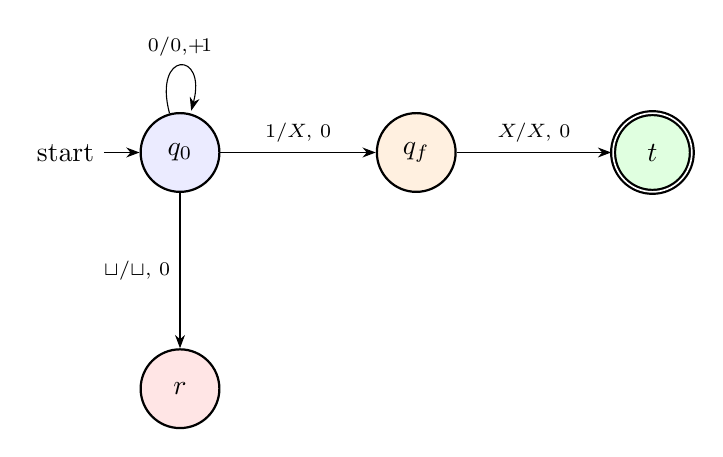
\begin{tikzpicture}[->, >=Stealth, node distance=3cm, every state/.style={thick, minimum size=1cm}]
    \node[state, initial, fill=blue!8]          (q0) {$q_0$};
    \node[state, fill=orange!12]                (qf) [right of=q0] {$q_f$};
    \node[state, accepting, fill=green!12]      (t)  [right of=qf] {$t$};
    \node[state, fill=red!10]                   (r)  [below of=q0] {$r$};

    \path (q0) edge [loop above]  node {\scriptsize $0/0,\!+\!1$} ()
          (q0) edge               node [above] {\scriptsize $1/X,\,0$} (qf)
          (q0) edge               node [left]  {\scriptsize $\sqcup/\sqcup,\,0$} (r)
          (qf) edge               node [above] {\scriptsize $X/X,\,0$} (t);
\end{tikzpicture}
\end{center}

\textit{Blue = scanning phase, orange = found-and-marked phase, green = accept, red = reject. The labels show read/write, direction. Note the ``$0$'' directions --- those are the stay moves we need to eliminate.}

\subsubsection{The Simulated Machine $M'$ (without Stay)}

Now we apply the construction from the previous subsection to build $M'$.

\begin{definitionbox}{Machine $M'$ --- Applying the Construction}
\textbf{Step 1 --- New state set:}
\fitmath{Q' = \{q_0, q_f, t, r\} \cup \{q_{0,L}, q_{f,L}, t_L, r_L\}}

We added four auxiliary states. (In practice, $q_{0,L}$ is never reached because $q_0$ is only ever the target of right-moving transitions. But the construction adds it uniformly.)

\textbf{Step 2 --- Transform each transition:}

\begin{center}
\begin{tabular}{lll}
\toprule
\textbf{Original $\delta$} & \textbf{Case} & \textbf{New $\delta'$} \\
\midrule
$\delta(q_0, 0) = (q_0, 0, +1)$ & Right & $\delta'(q_0, 0) = (q_0, 0, +1)$ \quad (unchanged) \\
$\delta(q_0, 1) = (q_f, X, 0)$  & \textbf{Stay} & $\delta'(q_0, 1) = (q_{f,L}, X, +1)$ \\
$\delta(q_0, \sqcup) = (r, \sqcup, 0)$ & \textbf{Stay} & $\delta'(q_0, \sqcup) = (r_L, \sqcup, +1)$ \\
$\delta(q_f, X) = (t, X, 0)$    & \textbf{Stay} & $\delta'(q_f, X) = (t_L, X, +1)$ \\
\bottomrule
\end{tabular}
\end{center}

\textbf{Step 3 --- Auxiliary state transitions} (for every symbol $a \in \Gamma$):

\begin{center}
\begin{tabular}{ll}
\toprule
\textbf{Auxiliary transition} & \textbf{Plain English} \\
\midrule
$\delta'(q_{f,L}, a) = (q_f, a, -1)$ & Go back left, enter $q_f$, don't change the cell \\
$\delta'(r_L, a) = (r, a, -1)$ & Go back left, enter $r$ (reject and halt) \\
$\delta'(t_L, a) = (t, a, -1)$ & Go back left, enter $t$ (accept and halt) \\
\bottomrule
\end{tabular}
\end{center}

These hold for \textbf{every} $a \in \{0, 1, X, \sqcup\}$. The auxiliary state doesn't care what it reads --- it always writes back the same symbol and goes left.
\end{definitionbox}

\begin{center}
\textbf{State diagram of $M'$:}

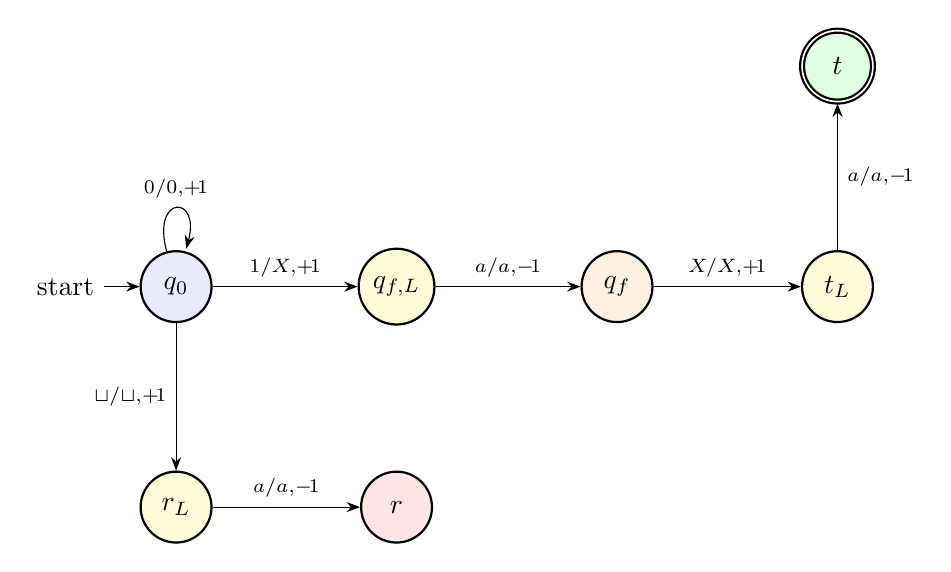
\begin{tikzpicture}[->, >=Stealth, node distance=2.8cm, every state/.style={thick, minimum size=0.9cm}]
    \node[state, initial, fill=blue!8]          (q0)  {$q_0$};
    \node[state, fill=yellow!15]                (qfL) [right of=q0] {$q_{f,L}$};
    \node[state, fill=orange!12]                (qf)  [right of=qfL] {$q_f$};
    \node[state, fill=yellow!15]                (tL)  [right of=qf] {$t_L$};
    \node[state, accepting, fill=green!12]      (t)   [above of=tL] {$t$};
    \node[state, fill=yellow!15]                (rL)  [below of=q0] {$r_L$};
    \node[state, fill=red!10]                   (r)   [right of=rL] {$r$};

    \path (q0)  edge [loop above]  node {\scriptsize $0/0,\!+\!1$} ()
          (q0)  edge               node [above] {\scriptsize $1/X,\!+\!1$} (qfL)
          (qfL) edge               node [above] {\scriptsize $a/a,\!-\!1$} (qf)
          (qf)  edge               node [above] {\scriptsize $X/X,\!+\!1$} (tL)
          (tL)  edge               node [right] {\scriptsize $a/a,\!-\!1$} (t)
          (q0)  edge               node [left]  {\scriptsize $\sqcup/\sqcup,\!+\!1$} (rL)
          (rL)  edge               node [above] {\scriptsize $a/a,\!-\!1$} (r);
\end{tikzpicture}
\end{center}

\textit{Yellow states = auxiliary ``bounce-back'' states. Every stay transition from $M$ became a two-step detour: right into a yellow state, then left back to the real state. The ``$a/a$'' label means ``read any symbol $a$, write it back unchanged.''}

\subsubsection{Tracing $M$ (with Stay) on Input ``01''}

\begin{examplebox}{Trace of $M$ on Input ``01'' --- With Stay}
\textbf{Setup:} Input is the string $01$. The tape initially contains $0$, $1$, then blanks forever. Head starts at position 1 in state $q_0$.

\textbf{Step 0 (Initial configuration):}
\begin{lstlisting}
    Tape: [ 0 | 1 | _ | _ | _ | ... ]
            ^
    State: q_0    Head at position: 1
\end{lstlisting}
Configuration: $[q_0, 01, 1]$

\textbf{Step 1:} Apply $\delta(q_0, 0) = (q_0, 0, +1)$ --- read $0$, write $0$, move right, stay in $q_0$.
\begin{lstlisting}
    Tape: [ 0 | 1 | _ | _ | _ | ... ]
                ^
    State: q_0    Head at position: 2
\end{lstlisting}
Configuration: $[q_0, 01, 2]$. The tape didn't change (we wrote $0$ over $0$). Head moved right.

\textbf{Step 2:} Apply $\delta(q_0, 1) = (q_f, X, 0)$ --- read $1$, write $X$, \textbf{STAY}, enter $q_f$.
\begin{lstlisting}
    Tape: [ 0 | X | _ | _ | _ | ... ]
                ^
    State: q_f    Head at position: 2
\end{lstlisting}
Configuration: $[q_f, 0X, 2]$. The $1$ at position 2 was replaced by $X$. Head \textbf{did not move} (direction $0$).

\textbf{Step 3:} Apply $\delta(q_f, X) = (t, X, 0)$ --- read $X$, write $X$, \textbf{STAY}, enter $t$.
\begin{lstlisting}
    Tape: [ 0 | X | _ | _ | _ | ... ]
                ^
    State: t    Head at position: 2    *** ACCEPT ***
\end{lstlisting}
Configuration: $[t, 0X, 2]$. Machine halts in accept state $t$.

\textbf{Result: $M$ accepts ``01'' in 3 steps.}
\end{examplebox}

\subsubsection{Tracing $M'$ (without Stay) on the Same Input ``01''}

\begin{examplebox}{Trace of $M'$ on Input ``01'' --- Without Stay}
\textbf{Setup:} Same input $01$. Same initial tape. But now we use $M'$, which has no stay transitions.

\textbf{Step 0 (Initial configuration):}
\begin{lstlisting}
    Tape: [ 0 | 1 | _ | _ | _ | ... ]
            ^
    State: q_0    Head at position: 1
\end{lstlisting}
Configuration: $[q_0, 01, 1]$

\textbf{Step 1:} Apply $\delta'(q_0, 0) = (q_0, 0, +1)$ --- \textit{same as original}. Read $0$, write $0$, move right.
\begin{lstlisting}
    Tape: [ 0 | 1 | _ | _ | _ | ... ]
                ^
    State: q_0    Head at position: 2
\end{lstlisting}
Configuration: $[q_0, 01, 2]$. Identical to $M$ so far.

\textbf{Step 2:} Apply $\delta'(q_0, 1) = (q_{f,L}, X, +1)$ --- this is the \textbf{simulation of the stay}. Read $1$, write $X$, move \textbf{RIGHT} (not stay!), enter auxiliary state $q_{f,L}$.
\begin{lstlisting}
    Tape: [ 0 | X | _ | _ | _ | ... ]
                    ^
    State: q_{f,L}    Head at position: 3
\end{lstlisting}
Configuration: $[q_{f,L}, 0X, 3]$. The $1$ was replaced by $X$ (same as $M$), but the head \textbf{overshot} to position 3. We are now in the auxiliary state $q_{f,L}$, which will take us back.

\textbf{Step 3:} Apply $\delta'(q_{f,L}, \sqcup) = (q_f, \sqcup, -1)$ --- the ``bounce back.'' Read $\sqcup$ (what happens to be at position 3), write $\sqcup$ back (no change!), move \textbf{LEFT}, enter $q_f$.
\begin{lstlisting}
    Tape: [ 0 | X | _ | _ | _ | ... ]
                ^
    State: q_f    Head at position: 2
\end{lstlisting}
Configuration: $[q_f, 0X, 2]$. Now compare with $M$ after Step 2: \textbf{same state} ($q_f$), \textbf{same tape} ($0X\sqcup\ldots$), \textbf{same head position} (2). We are back in sync!

\textbf{Step 4:} Apply $\delta'(q_f, X) = (t_L, X, +1)$ --- another stay simulation. Read $X$, write $X$, move \textbf{RIGHT}, enter auxiliary state $t_L$.
\begin{lstlisting}
    Tape: [ 0 | X | _ | _ | _ | ... ]
                    ^
    State: t_L    Head at position: 3
\end{lstlisting}
Configuration: $[t_L, 0X, 3]$. Head overshot again.

\textbf{Step 5:} Apply $\delta'(t_L, \sqcup) = (t, \sqcup, -1)$ --- bounce back. Read $\sqcup$, write $\sqcup$ (no change), move \textbf{LEFT}, enter $t$.
\begin{lstlisting}
    Tape: [ 0 | X | _ | _ | _ | ... ]
                ^
    State: t    Head at position: 2    *** ACCEPT ***
\end{lstlisting}
Configuration: $[t, 0X, 2]$. Machine halts in accept state $t$.

\textbf{Result: $M'$ accepts ``01'' in 5 steps.}
\end{examplebox}

\subsubsection{Side-by-Side Comparison}

\begin{examplebox}{$M$ vs.\ $M'$ --- Step-by-Step Comparison on Input ``01''}

\begin{center}
\begin{tabular}{clcclc}
\toprule
\textbf{$M$ step} & \textbf{State} & \textbf{Head} & \textbf{$M'$ step} & \textbf{State} & \textbf{Head} \\
\midrule
0 & $q_0$ & 1 & 0 & $q_0$ & 1 \\
1 & $q_0$ & 2 & 1 & $q_0$ & 2 \\
2 & $q_f$ & 2 (stay) & 2 & $q_{f,L}$ & 3 (overshoot) \\
  &       &          & 3 & $q_f$ & 2 (bounce back) \\
3 & $t$ (accept) & 2 (stay) & 4 & $t_L$ & 3 (overshoot) \\
  &              &            & 5 & $t$ (accept) & 2 (bounce back) \\
\bottomrule
\end{tabular}
\end{center}

\textbf{Observations:}
\begin{itemize}[nosep]
\item Right-move steps (step 1) are \textbf{identical} in both machines.
\item Each stay step in $M$ becomes \textbf{two steps} in $M'$: overshoot right, then bounce back left.
\item After each bounce-back, the configurations are \textbf{synchronized}: same state, same tape, same head position.
\item The tape at the end is identical: $[0 \mid X \mid \sqcup \mid \ldots]$ in both cases.
\item $M$ took \textbf{3 steps}. $M'$ took \textbf{5 steps}. Same result.
\end{itemize}
\end{examplebox}

\subsubsection{Second Trace: Rejecting Input ``00''}

To be thorough, let us also trace a rejecting input to see that the simulation works for rejection too.

\begin{examplebox}{Trace on Input ``00'' --- Both Machines Reject}

\textbf{Machine $M$ (with stay):}
\begin{lstlisting}
    Step 0: [ 0 | 0 | _ | _ | ... ]    Head: 1, State: q_0
                                         ^
    Step 1: delta(q_0, 0) = (q_0, 0, +1)
            [ 0 | 0 | _ | _ | ... ]    Head: 2, State: q_0
    Step 2: delta(q_0, 0) = (q_0, 0, +1)
            [ 0 | 0 | _ | _ | ... ]    Head: 3, State: q_0
    Step 3: delta(q_0, _) = (r, _, 0)   <-- STAY, reject
            [ 0 | 0 | _ | _ | ... ]    Head: 3, State: r  *** REJECT ***
\end{lstlisting}
$M$ rejects ``$00$'' in 3 steps.

\textbf{Machine $M'$ (without stay):}
\begin{lstlisting}
    Step 0: [ 0 | 0 | _ | _ | ... ]    Head: 1, State: q_0
    Step 1: delta'(q_0, 0) = (q_0, 0, +1)        (same)
            [ 0 | 0 | _ | _ | ... ]    Head: 2, State: q_0
    Step 2: delta'(q_0, 0) = (q_0, 0, +1)        (same)
            [ 0 | 0 | _ | _ | ... ]    Head: 3, State: q_0
    Step 3: delta'(q_0, _) = (r_L, _, +1)         (overshoot!)
            [ 0 | 0 | _ | _ | ... ]    Head: 4, State: r_L
    Step 4: delta'(r_L, _) = (r, _, -1)           (bounce back)
            [ 0 | 0 | _ | _ | ... ]    Head: 3, State: r  *** REJECT ***
\end{lstlisting}
$M'$ rejects ``$00$'' in 4 steps. Same tape, same final state, same head position.
\end{examplebox}


%───────────────────────────────────────────────────────────────────────────────
\subsection{Why the Simulation Is Correct}
%───────────────────────────────────────────────────────────────────────────────

\begin{conceptbox}{Correctness Argument \kemark}
We need to show: $M$ and $M'$ accept (and reject, and loop on) exactly the same inputs. Here is the argument:

\textbf{Case 1: Left/Right transitions.} If $\delta(q, a) = (q', b, d)$ with $d \in \{-1, +1\}$, then $\delta'(q, a) = (q', b, d)$. The transition is \textbf{identical}. Same state, same write, same move. Nothing changes.

\textbf{Case 2: Stay transitions.} If $\delta(q, a) = (q', b, 0)$, then in $M'$:
\begin{enumerate}[nosep]
\item $\delta'(q, a) = (q'_L, b, +1)$: write $b$, move right, enter auxiliary state.
\item $\delta'(q'_L, c) = (q', c, -1)$: write $c$ back (no change to cell), move left, enter $q'$.
\end{enumerate}

After these two steps, $M'$ is in state $q'$, the head is back at the original position, and the tape is identical to what $M$ would have produced. The cell to the right was read and re-written with its own symbol --- untouched.

\textbf{Therefore:} After every ``real'' transition of $M$ (counting each stay as one logical step), there is a corresponding point in $M'$'s execution where the configuration matches exactly (same state, same tape, same head position). The auxiliary states are just ``in transit'' --- they never affect the tape and never persist.

\textbf{Consequences:}
\begin{itemize}[nosep]
\item \textbf{If $M$ halts in $t$} $\Rightarrow$ $M'$ also reaches $t$ (via possibly $t_L$ first). Same for $r$.
\item \textbf{If $M$ loops forever} $\Rightarrow$ $M'$ also loops (each step of $M$ becomes 1 or 2 steps of $M'$, so $M'$ never halts either).
\item \textbf{$M'$ uses at most $2n$ steps} for $n$ steps of $M$ (each stay costs 2 steps, each left/right costs 1). So $M'$ is at most twice as slow.
\end{itemize}

\kt{$L(M) = L(M')$. The extended DTM with stay recognizes and decides exactly the same languages as the standard DTM. The stay direction is ``free to use'' --- it's syntactic sugar.}
\end{conceptbox}

\begin{notebox}{The Lecture Says: ``We Will Use Direction 0 From Now On''}
Slide 14 concludes with a license: \textit{``We will use direction 0 from now on in our Turing machines (whenever convenient).''}

This is the power of a robustness proof. Once you have proven that the extension doesn't change what the machine can compute, you can \textbf{freely use the extension} in all future TM designs without worrying about whether it ``counts.'' It's like proving that a shortcut through the park gets you to the same destination as the main road --- once proven, you can take the shortcut whenever you want.

Every robustness proof in this lecture follows the same logic:
\begin{enumerate}[nosep]
\item Define the extension (what new feature are we adding?)
\item Build a simulation (how does a standard TM mimic the extension?)
\item Trace a concrete example (does the simulation actually work?)
\item Argue correctness (same language, same halting behavior)
\end{enumerate}

We will repeat this exact four-step pattern for multi-tape TMs (Section 4), non-deterministic TMs (Section 5), and doubly-infinite tape TMs (Section 6).
\end{notebox}

\kt{Template for ALL robustness proofs: (1) define the extension, (2) build a simulation with auxiliary states/encoding, (3) trace it on a concrete example, (4) argue correctness. Master this template now --- you will use it at least three more times in this lecture alone.}

\newpage
%═══════════════════════════════════════════════════════════════════════════════
\section{Multi-Tape Turing Machines --- More Convenient, Equally Powerful}
%═══════════════════════════════════════════════════════════════════════════════

This is the biggest section of Lecture 2 and the one that matters most for building intuition about the Church--Turing thesis. The punchline: giving a TM more tapes makes programming \textit{easier} but does not let it solve any new problems. We will prove this by building a single-tape machine that \textit{simulates} any multi-tape machine step by step.

%───────────────────────────────────────────────────────────────────────────────
\subsection{Why Do We Want Multiple Tapes?}
%───────────────────────────────────────────────────────────────────────────────

\begin{notebox}{Analogy --- Long Division on a Single Strip of Paper}
Imagine you have to do long division --- but you are only allowed to use \textbf{one long horizontal strip of paper}. Your dividend, divisor, quotient, remainder, and scratch work all have to share the same strip. Every time you need to compare the divisor against the current partial remainder, you have to scroll left to re-read the divisor, then scroll right back to where you were. Need the quotient? Scroll further right. Need the dividend digits? Scroll left again.

You spend most of your time \textbf{scanning back and forth} rather than doing useful arithmetic. The actual division takes maybe 10 operations, but the scanning takes hundreds.

Now imagine you have \textbf{four separate strips}: one for the dividend, one for the divisor, one for the quotient, one for scratch work. Each strip has its own pointer (your finger). You can look at all four simultaneously. You never scan --- you just glance at each strip. The \textit{same} division now takes a fraction of the time.

\textbf{In our formal world:}
\begin{itemize}[nosep]
\item strips of paper = \textbf{tapes}
\item your finger on each strip = \textbf{independent read/write head}
\item scanning back and forth = \textbf{O(n) head movements per comparison}
\item separate strips = \textbf{separate tapes, each with its own head}
\item one brain doing the division = \textbf{one finite-state control}
\end{itemize}
\end{notebox}

\subsubsection{Recap: The Pain of Single-Tape $w\#w$}

In Lecture 1, we discussed the language $L = \{w\#w \mid w \in \{0,1\}^*\}$ --- the set of strings of the form ``a binary word, then a hash, then the same binary word again.'' A single-tape TM that decides this language works roughly as follows:

\begin{enumerate}[nosep]
\item Scan to the rightmost unmarked symbol on the right half (after $\#$).
\item \textbf{Remember it in the state}: enter state $q_\ell^0$ if it was 0, or $q_\ell^1$ if it was 1. Mark the cell (e.g.\ replace 0 with X).
\item Scan left past $\#$ to find the rightmost unmarked symbol on the left half.
\item \textbf{Compare}: if the remembered symbol matches, mark this cell too and go back to step 1. If it does not match, \textbf{reject}.
\item Repeat until all symbols on both sides are marked. If both halves are fully consumed, \textbf{accept}.
\end{enumerate}

\begin{conceptbox}{Why This Is Painfully Slow}
Each ``round'' of the algorithm compares \textit{one} pair of symbols. To compare them, the head must travel from the right half all the way to the left half and back --- a journey of $O(n)$ cells (where $n = |w\#w|$). There are $O(n)$ symbols to compare, so the total number of head movements is:

\fitmath{O(n) \text{ rounds} \times O(n) \text{ cells per round} = O(n^2) \text{ total steps}}

For a 100-symbol input, that is roughly 10{,}000 steps. For a 1{,}000-symbol input, roughly 1{,}000{,}000 steps. The machine spends most of its time \textit{moving}, not \textit{thinking}.

\kt{The single-tape $w\#w$ machine is $O(n^2)$ because it has to scan back and forth between the two halves for every single symbol comparison. The tape is the bottleneck.}
\end{conceptbox}

\subsubsection{Preview: A 2-Tape Machine Does It in $O(n)$}

What if we had \textbf{two tapes}, each with its own head?

\begin{itemize}[nosep]
\item \textbf{Tape 1} holds the original input $w\#w$.
\item \textbf{Tape 2} is initially blank --- we will use it as ``scratch paper.''
\end{itemize}

The strategy is beautifully simple:
\begin{enumerate}[nosep]
\item \textbf{Phase 1 (Copy):} Scan tape 1 left to right. Copy each symbol before $\#$ onto tape 2. When you hit $\#$, stop copying.
\item \textbf{Phase 2 (Rewind):} Move tape 2's head back to the start. Move tape 1's head one cell past $\#$.
\item \textbf{Phase 3 (Compare):} Move both heads right simultaneously. At each step, compare the symbol under tape 1's head with the symbol under tape 2's head. If they ever differ, \textbf{reject}. If both reach blank simultaneously, \textbf{accept}.
\end{enumerate}

Each phase does a single left-to-right pass --- that is $O(n)$ steps. Three passes, each $O(n)$, gives $O(n)$ total. \textbf{The same language, solved with the same correctness, but an entire order of magnitude faster.}

\kt{Two tapes turn an $O(n^2)$ scan-and-compare nightmare into a clean $O(n)$ copy-rewind-compare pipeline. This is why we want multi-tape TMs: not more power, but more convenience.}


%───────────────────────────────────────────────────────────────────────────────
\subsection{The 2-Tape TM for $w\#w$: How It Works}
%───────────────────────────────────────────────────────────────────────────────

\begin{notebox}{Analogy --- Two Scrolls and a Scribe}
Imagine a medieval scribe who receives a long scroll with a message. The message reads ``HELLO\#HELLO'' --- a word, a separator mark, and (supposedly) the same word repeated. The scribe's task is to verify the repetition.

With \textbf{one scroll}, the scribe has to keep rolling back and forth between the two copies to compare letter by letter. Exhausting.

With \textbf{two scrolls}, the scribe copies everything before the $\#$ onto a fresh scroll. Then he places both scrolls side by side and reads them in parallel, checking letter by letter. One pass and done.

\textbf{In our formal world:}
\begin{itemize}[nosep]
\item the two scrolls = \textbf{tape 1} and \textbf{tape 2}
\item copying before $\#$ = \textbf{Phase 1 (Copy)}
\item rolling the second scroll back to the start = \textbf{Phase 2 (Rewind)}
\item reading both in parallel = \textbf{Phase 3 (Compare)}
\item the scribe's brain = \textbf{finite-state control} (one state at a time)
\end{itemize}
\end{notebox}

Let us now describe the machine precisely. We use the following states:

\begin{center}
\begin{tabular}{cl}
\toprule
\textbf{State} & \textbf{Meaning} \\
\midrule
$s$ & Start / Copy phase --- scanning tape 1, copying to tape 2 \\
$q_r$ & Rewind phase --- moving tape 2's head back to the start \\
$q_c$ & Compare phase --- reading both tapes simultaneously \\
$t$ & Accept (halt) \\
$r$ & Reject (halt) \\
\bottomrule
\end{tabular}
\end{center}

\textbf{Alphabet:} $\Sigma = \{0, 1, \#\}$. Tape alphabet $\Gamma = \{0, 1, \#, 0', 1', \sqcup\}$, where $0'$ and $1'$ are ``primed'' versions used to mark the starting cell of tape 2 (so the rewind phase knows where to stop).

\bigskip

\begin{definitionbox}{Phase 1 --- Copy (State $s$)}
\textbf{Plain English:} Read each symbol on tape 1 from left to right. For every 0 or 1 you see, write a copy on tape 2 and advance both heads. The very first symbol copied to tape 2 gets a ``prime'' mark (e.g., $0'$ or $1'$) so we can find the beginning of tape 2 later. When you reach $\#$ on tape 1, stop copying and transition to the rewind phase.

\textbf{Transitions:}
\begin{itemize}[nosep]
\item $\delta(s,\;(0,\sqcup)) = (s,\;(0, 0'),\;(+1, +1))$ \quad [first cell: write $0'$ on tape 2]
\item $\delta(s,\;(1,\sqcup)) = (s,\;(1, 1'),\;(+1, +1))$ \quad [first cell: write $1'$ on tape 2]
\item $\delta(s,\;(0,0')) = (s,\;(0, 0),\;(+1, +1))$ \quad [subsequent 0: write plain 0 on tape 2]
\item $\delta(s,\;(0,1')) = (s,\;(0, 0),\;(+1, +1))$ \quad [same idea]
\item $\delta(s,\;(1,0')) = (s,\;(1, 1),\;(+1, +1))$
\item $\delta(s,\;(1,1')) = (s,\;(1, 1),\;(+1, +1))$
\item Generally: for $a \in \{0,1\}$ and any non-blank tape-2 symbol, write $a$ on tape 2, move both right.
\item $\delta(s,\;(\#,\text{any})) = (q_r,\;(\#, \text{any}),\;(+1, 0))$ \quad [hit $\#$: move tape 1 past it, enter rewind]
\end{itemize}

\textbf{Simplification:} For clarity in our trace, we will handle the priming more simply. The first symbol written to tape 2 is primed; all subsequent ones are unprimed. When we hit $\#$ on tape 1, we move tape 1 one step right (past $\#$) and stop tape 2.
\end{definitionbox}

\begin{definitionbox}{Phase 2 --- Rewind (State $q_r$)}
\textbf{Plain English:} Move tape 2's head left until it hits a primed symbol ($0'$ or $1'$). Tape 1's head stays where it is (one cell past $\#$). When the primed symbol is found, we are at the beginning of tape 2. Transition to the compare phase.

\textbf{Transitions:}
\begin{itemize}[nosep]
\item $\delta(q_r,\;(\text{any},\;a))$ for $a \in \{0,1\}$: stay in $q_r$, move tape 2 left. Tape 1 stays.
\item $\delta(q_r,\;(\text{any},\;a'))$ for $a' \in \{0',1'\}$: transition to $q_c$. Both heads stay.
\end{itemize}
\end{definitionbox}

\begin{definitionbox}{Phase 3 --- Compare (State $q_c$)}
\textbf{Plain English:} Move both heads right simultaneously. At each step, compare the symbol under tape 1's head with the symbol under tape 2's head (ignoring the prime mark on the first tape-2 cell). If they match, continue. If they differ, reject. If both are blank, accept.

\textbf{Transitions:}
\begin{itemize}[nosep]
\item $\delta(q_c,\;(0, 0')) = (q_c,\;(0, 0'),\;(+1, +1))$ \quad [first cell: 0 matches $0'$, continue]
\item $\delta(q_c,\;(1, 1')) = (q_c,\;(1, 1'),\;(+1, +1))$ \quad [first cell: 1 matches $1'$, continue]
\item $\delta(q_c,\;(0, 0)) = (q_c,\;(0, 0),\;(+1, +1))$ \quad [0 matches 0, continue]
\item $\delta(q_c,\;(1, 1)) = (q_c,\;(1, 1),\;(+1, +1))$ \quad [1 matches 1, continue]
\item $\delta(q_c,\;(\sqcup, \sqcup)) = (t,\;(\sqcup, \sqcup),\;(0, 0))$ \quad [both blank: accept!]
\item $\delta(q_c,\;(0, 1)) = (r,\;\ldots)$, \;$\delta(q_c,\;(1, 0)) = (r,\;\ldots)$ \quad [mismatch: reject]
\item $\delta(q_c,\;(0, 1')) = (r,\;\ldots)$, \;$\delta(q_c,\;(1, 0')) = (r,\;\ldots)$ \quad [mismatch: reject]
\item $\delta(q_c,\;(\sqcup, a)) = (r,\;\ldots)$ for $a \neq \sqcup$ \quad [tape 1 ended early: reject]
\item $\delta(q_c,\;(a, \sqcup)) = (r,\;\ldots)$ for $a \neq \sqcup$ \quad [tape 2 ended early: reject]
\end{itemize}
\end{definitionbox}


%───────────────────────────────────────────────────────────────────────────────
\subsection{Full Trace on Input $011\#011$ (Accepting)}
%───────────────────────────────────────────────────────────────────────────────

\begin{examplebox}{{Full Trace: 2-Tape TM on Input $011\#011$ --- ACCEPT}}
We trace every single step. Both tapes are shown. The caret (\texttt{\^{}}) marks each head's position. Tape 2 starts entirely blank.

\textbf{--- Phase 1: Copy ---}

\begin{lstlisting}
Step 0: State = s
  Tape 1: [ 0 | 1 | 1 | # | 0 | 1 | 1 | _ | ... ]
            ^
  Tape 2: [ _ | _ | _ | _ | _ | _ | _ | _ | ... ]
            ^
  Read: (tape1=0, tape2=_)
  This is the FIRST symbol copied, so tape 2 gets a prime.
  Transition: d(s, (0,_)) = (s, (0, 0'), (+1,+1))
  Action: Write 0 on tape 1 (no change), write 0' on tape 2.
          Move both heads right.
\end{lstlisting}

\begin{lstlisting}
Step 1: State = s
  Tape 1: [ 0 | 1 | 1 | # | 0 | 1 | 1 | _ | ... ]
                ^
  Tape 2: [ 0'| _ | _ | _ | _ | _ | _ | _ | ... ]
                ^
  Read: (tape1=1, tape2=_)
  Transition: d(s, (1,_)) = (s, (1, 1), (+1,+1))
  Action: Write 1 on tape 1 (no change), write 1 on tape 2.
          Move both heads right.
\end{lstlisting}

\begin{lstlisting}
Step 2: State = s
  Tape 1: [ 0 | 1 | 1 | # | 0 | 1 | 1 | _ | ... ]
                    ^
  Tape 2: [ 0'| 1 | _ | _ | _ | _ | _ | _ | ... ]
                    ^
  Read: (tape1=1, tape2=_)
  Transition: d(s, (1,_)) = (s, (1, 1), (+1,+1))
  Action: Write 1 on tape 2. Move both heads right.
\end{lstlisting}

\begin{lstlisting}
Step 3: State = s
  Tape 1: [ 0 | 1 | 1 | # | 0 | 1 | 1 | _ | ... ]
                        ^
  Tape 2: [ 0'| 1 | 1 | _ | _ | _ | _ | _ | ... ]
                        ^
  Read: (tape1=#, tape2=_)
  We hit #! Copy phase is DONE.
  Transition: d(s, (#,_)) = (q_r, (#,_), (+1, 0))
  Action: Move tape 1 head right (past #). Tape 2 head STAYS.
\end{lstlisting}

\textbf{Copy phase complete.} Tape 2 now holds $0'11$ --- a copy of $w = 011$ with the first cell primed.

\bigskip
\textbf{--- Phase 2: Rewind ---}

\begin{lstlisting}
Step 4: State = q_r
  Tape 1: [ 0 | 1 | 1 | # | 0 | 1 | 1 | _ | ... ]
                            ^
  Tape 2: [ 0'| 1 | 1 | _ | _ | _ | _ | _ | ... ]
                        ^
  Read: (tape1=0, tape2=1)
  tape2 symbol is 1 (not primed) -- keep rewinding.
  Transition: d(q_r, (0,1)) = (q_r, (0,1), (0,-1))
  Action: Tape 1 stays. Tape 2 moves LEFT.
\end{lstlisting}

\begin{lstlisting}
Step 5: State = q_r
  Tape 1: [ 0 | 1 | 1 | # | 0 | 1 | 1 | _ | ... ]
                            ^
  Tape 2: [ 0'| 1 | 1 | _ | _ | _ | _ | _ | ... ]
                ^
  Read: (tape1=0, tape2=1)
  tape2 symbol is 1 (not primed) -- keep rewinding.
  Transition: d(q_r, (0,1)) = (q_r, (0,1), (0,-1))
  Action: Tape 1 stays. Tape 2 moves LEFT.
\end{lstlisting}

\begin{lstlisting}
Step 6: State = q_r
  Tape 1: [ 0 | 1 | 1 | # | 0 | 1 | 1 | _ | ... ]
                            ^
  Tape 2: [ 0'| 1 | 1 | _ | _ | _ | _ | _ | ... ]
            ^
  Read: (tape1=0, tape2=0')
  tape2 symbol is 0' (PRIMED!) -- we found the start of tape 2!
  Transition: d(q_r, (0,0')) = (q_c, (0,0'), (0,0))
  Action: Both heads STAY. Enter compare phase.
\end{lstlisting}

\textbf{Rewind complete.} Tape 1's head is on the first symbol after $\#$ (which is 0). Tape 2's head is on $0'$ (the start). We are perfectly aligned to compare.

\bigskip
\textbf{--- Phase 3: Compare ---}

\begin{lstlisting}
Step 7: State = q_c
  Tape 1: [ 0 | 1 | 1 | # | 0 | 1 | 1 | _ | ... ]
                            ^
  Tape 2: [ 0'| 1 | 1 | _ | _ | _ | _ | _ | ... ]
            ^
  Read: (tape1=0, tape2=0')
  Compare: 0 vs 0' -- MATCH (0' is just 0 with a prime mark).
  Transition: d(q_c, (0,0')) = (q_c, (0,0'), (+1,+1))
  Action: Move both heads right.
\end{lstlisting}

\begin{lstlisting}
Step 8: State = q_c
  Tape 1: [ 0 | 1 | 1 | # | 0 | 1 | 1 | _ | ... ]
                                ^
  Tape 2: [ 0'| 1 | 1 | _ | _ | _ | _ | _ | ... ]
                ^
  Read: (tape1=1, tape2=1)
  Compare: 1 vs 1 -- MATCH.
  Transition: d(q_c, (1,1)) = (q_c, (1,1), (+1,+1))
  Action: Move both heads right.
\end{lstlisting}

\begin{lstlisting}
Step 9: State = q_c
  Tape 1: [ 0 | 1 | 1 | # | 0 | 1 | 1 | _ | ... ]
                                    ^
  Tape 2: [ 0'| 1 | 1 | _ | _ | _ | _ | _ | ... ]
                    ^
  Read: (tape1=1, tape2=1)
  Compare: 1 vs 1 -- MATCH.
  Transition: d(q_c, (1,1)) = (q_c, (1,1), (+1,+1))
  Action: Move both heads right.
\end{lstlisting}

\begin{lstlisting}
Step 10: State = q_c
  Tape 1: [ 0 | 1 | 1 | # | 0 | 1 | 1 | _ | ... ]
                                        ^
  Tape 2: [ 0'| 1 | 1 | _ | _ | _ | _ | _ | ... ]
                        ^
  Read: (tape1=_, tape2=_)
  Both blanks simultaneously! Both halves fully consumed.
  Transition: d(q_c, (_,_)) = (t, (_,_), (0,0))
  Action: Enter state t. ACCEPT!
\end{lstlisting}

\kt{The 2-tape machine accepted $011\#011$ in \textbf{11 steps} (steps 0--10). A single-tape machine on this 7-symbol input would need roughly $7^2 / 2 \approx 25$ steps of scanning back and forth. On longer inputs, the difference is dramatic.}
\end{examplebox}

\bigskip

\begin{examplebox}{{Full Trace: 2-Tape TM on Input $01\#00$ --- REJECT}}
Now let us trace a \textbf{rejecting} input. The left half is $01$ and the right half is $00$. Since $01 \neq 00$, the machine should reject.

\textbf{--- Phase 1: Copy ---}

\begin{lstlisting}
Step 0: State = s
  Tape 1: [ 0 | 1 | # | 0 | 0 | _ | _ | ... ]
            ^
  Tape 2: [ _ | _ | _ | _ | _ | _ | _ | ... ]
            ^
  Read: (tape1=0, tape2=_). First copy: prime it.
  Transition: d(s, (0,_)) = (s, (0,0'), (+1,+1))
\end{lstlisting}

\begin{lstlisting}
Step 1: State = s
  Tape 1: [ 0 | 1 | # | 0 | 0 | _ | _ | ... ]
                ^
  Tape 2: [ 0'| _ | _ | _ | _ | _ | _ | ... ]
                ^
  Read: (tape1=1, tape2=_)
  Transition: d(s, (1,_)) = (s, (1,1), (+1,+1))
\end{lstlisting}

\begin{lstlisting}
Step 2: State = s
  Tape 1: [ 0 | 1 | # | 0 | 0 | _ | _ | ... ]
                    ^
  Tape 2: [ 0'| 1 | _ | _ | _ | _ | _ | ... ]
                    ^
  Read: (tape1=#, tape2=_). Hit #!
  Transition: d(s, (#,_)) = (q_r, (#,_), (+1,0))
  Action: Tape 1 moves right past #. Tape 2 stays.
\end{lstlisting}

\textbf{Copy complete.} Tape 2 holds $0'1$.

\textbf{--- Phase 2: Rewind ---}

\begin{lstlisting}
Step 3: State = q_r
  Tape 1: [ 0 | 1 | # | 0 | 0 | _ | _ | ... ]
                        ^
  Tape 2: [ 0'| 1 | _ | _ | _ | _ | _ | ... ]
                    ^
  Read: (tape1=0, tape2=1). Not primed -- keep rewinding.
  Transition: d(q_r, (0,1)) = (q_r, (0,1), (0,-1))
\end{lstlisting}

\begin{lstlisting}
Step 4: State = q_r
  Tape 1: [ 0 | 1 | # | 0 | 0 | _ | _ | ... ]
                        ^
  Tape 2: [ 0'| 1 | _ | _ | _ | _ | _ | ... ]
            ^
  Read: (tape1=0, tape2=0'). Primed! Found start.
  Transition: d(q_r, (0,0')) = (q_c, (0,0'), (0,0))
\end{lstlisting}

\textbf{Rewind complete.} Tape 1 points to the first 0 after $\#$. Tape 2 points to $0'$.

\textbf{--- Phase 3: Compare ---}

\begin{lstlisting}
Step 5: State = q_c
  Tape 1: [ 0 | 1 | # | 0 | 0 | _ | _ | ... ]
                        ^
  Tape 2: [ 0'| 1 | _ | _ | _ | _ | _ | ... ]
            ^
  Read: (tape1=0, tape2=0')
  Compare: 0 vs 0' -- MATCH. Continue.
  Transition: d(q_c, (0,0')) = (q_c, (0,0'), (+1,+1))
\end{lstlisting}

\begin{lstlisting}
Step 6: State = q_c
  Tape 1: [ 0 | 1 | # | 0 | 0 | _ | _ | ... ]
                            ^
  Tape 2: [ 0'| 1 | _ | _ | _ | _ | _ | ... ]
                ^
  Read: (tape1=0, tape2=1)
  Compare: 0 vs 1 -- MISMATCH!
  Transition: d(q_c, (0,1)) = (r, (0,1), (0,0))
  Action: Enter state r. REJECT!
\end{lstlisting}

\textbf{The machine caught the mismatch at the second symbol.} The left half's second symbol was 1 (copied as tape 2's second cell), but the right half's second symbol was 0. The machine rejected in just \textbf{7 steps} (steps 0--6). It did not even need to read the rest of the input.

\kt{On a mismatch, the 2-tape machine rejects as soon as it finds the first differing symbol. It does not waste time scanning the rest. This ``early exit'' is natural with two tapes but hard to achieve with one tape (where you would have already committed to a particular scanning pattern).}
\end{examplebox}


%───────────────────────────────────────────────────────────────────────────────
\subsection{The Formal Definition: $k$-Tape Deterministic Turing Machine}
%───────────────────────────────────────────────────────────────────────────────

\begin{notebox}{Analogy --- A Chef with $k$ Cutting Boards}
Imagine a chef with $k$ cutting boards laid out on the counter. On each cutting board, there is a row of ingredients (or blank spaces). The chef has $k$ knives, one resting on each board, pointing at a specific ingredient. At each moment, the chef:
\begin{enumerate}[nosep]
\item Looks at all $k$ knives simultaneously to see which ingredient each one is pointing at.
\item Consults a single recipe book (one brain!) to decide what to do next.
\item On each board, the knife can: replace the ingredient with a different one, then slide one position left, stay, or slide one position right.
\end{enumerate}

The chef has only \textbf{one brain} (one state) even though there are many cutting boards. The recipe book (transition function) takes as input ``what I see on ALL boards right now'' and outputs ``what to do on ALL boards.''

\textbf{In our formal world:}
\begin{itemize}[nosep]
\item $k$ cutting boards = $k$ \textbf{tapes}
\item $k$ knives = $k$ \textbf{read/write heads}
\item one brain / one recipe book = \textbf{one state} $q \in Q$
\item looking at all boards at once = reading a \textbf{$k$-tuple} from $\Gamma^k$
\item the recipe's instruction for each board = writing a \textbf{$k$-tuple} and moving each head independently
\end{itemize}
\end{notebox}

\begin{definitionbox}{$k$-Tape Deterministic Turing Machine ($k$-tape DTM)}

\textbf{Plain English:}
A $k$-tape DTM is a Turing machine with $k$ separate tapes, each with its own read/write head. All heads are controlled by a single finite-state control. At each step, the machine reads the symbol under \textit{every} head, consults the transition function, and then writes a symbol on \textit{every} tape and moves \textit{every} head --- all in one step.

\textbf{Formal Definition:}

A $k$-tape DTM is a tuple $M = (Q,\;\Sigma,\;\Gamma,\;s,\;t,\;r,\;\delta)$ where:
\begin{itemize}[nosep]
\item $Q$ is the finite set of states
\item $\Sigma$ is the input alphabet ($\Sigma \subseteq \Gamma$, does not contain $\sqcup$)
\item $\Gamma$ is the tape alphabet ($\sqcup \in \Gamma$)
\item $s \in Q$ is the start state
\item $t \in Q$ is the accept state
\item $r \in Q$ is the reject state ($r \neq t$)
\item $\delta$ is the transition function:
\end{itemize}

\fitmath{\delta \colon (Q \setminus \{t,r\}) \times \Gamma^k \;\longrightarrow\; Q \times \Gamma^k \times \{-1, 0, +1\}^k}

\textbf{Breaking Down the Notation:}
\begin{itemize}[nosep]
\item $Q \setminus \{t,r\}$ --- the machine only transitions when it is \textit{not} in a halting state (accept or reject).
\item $\Gamma^k$ (input side) --- the machine reads a \textbf{$k$-tuple} of symbols, one from each tape. For $k = 2$: $(a_1, a_2)$ where $a_i \in \Gamma$.
\item $Q$ (output side) --- the new state to enter.
\item $\Gamma^k$ (output side) --- the \textbf{$k$-tuple} of symbols to write, one on each tape.
\item $\{-1, 0, +1\}^k$ --- the \textbf{$k$-tuple} of head movements. Each head independently moves left ($-1$), stays ($0$), or moves right ($+1$).
\end{itemize}

\textbf{Input convention:} The input is written on \textbf{tape 1} only. All other tapes start blank (filled with $\sqcup$).

\textbf{Example transition from our $w\#w$ machine:}

\fitmath{\delta(s,\;(1, \sqcup)) = (s,\;(1, 1),\;(+1, +1))}

This says: ``In state $s$, reading 1 on tape 1 and $\sqcup$ on tape 2, stay in state $s$, write 1 on tape 1 (no change), write 1 on tape 2 (copy!), and move both heads right.''

\textbf{Connection to standard TMs:} A 1-tape DTM is exactly the standard DTM from Lecture 1:

\fitmath{\delta \colon (Q \setminus \{t,r\}) \times \Gamma^1 \;\longrightarrow\; Q \times \Gamma^1 \times \{-1, 0, +1\}^1}

which simplifies to $\delta \colon (Q \setminus \{t,r\}) \times \Gamma \longrightarrow Q \times \Gamma \times \{-1, 0, +1\}$. This is the exact same definition from Lecture 1.

\kt{A $k$-tape DTM has $k$ tapes and $k$ heads, but only ONE state. The transition function reads ALL $k$ tapes at once and moves ALL $k$ heads at once. It is a natural generalization of the 1-tape DTM --- set $k=1$ and you recover the Lecture 1 definition exactly.}
\end{definitionbox}


%───────────────────────────────────────────────────────────────────────────────
\subsection{The Simulation Theorem}
%───────────────────────────────────────────────────────────────────────────────

\begin{conceptbox}{The Simulation Theorem --- Multi-Tape Adds No Power}

\textbf{Analogy:} You can do everything with one cutting board that you can do with five --- it is just slower and messier. No recipe becomes \textit{impossible} because you only have one board. You might have to clean and reuse the board between steps, but every dish can still be cooked.

\textbf{Theorem (Simulation).} For every $k$-tape DTM $M$, there exists a standard (1-tape) DTM $M'$ such that $M'$ \textbf{outcome-simulates} $M$. That is:
\begin{itemize}[nosep]
\item $M'$ accepts input $w$ if and only if $M$ accepts $w$.
\item $M'$ rejects input $w$ if and only if $M$ rejects $w$.
\item $M'$ diverges on input $w$ if and only if $M$ diverges on $w$.
\end{itemize}

\textbf{Plain English:} Anything a multi-tape TM can compute, a single-tape TM can also compute. The single-tape machine will be slower (more steps), but it will always produce the \textit{same} answer.

\textbf{Immediate consequences:}

\begin{itemize}[nosep]
\item A language is \textbf{computable} (decidable) if and only if it is the language of some halting $k$-tape DTM.
\item A language is \textbf{computably enumerable} (c.e.) if and only if it is the language of some $k$-tape DTM.
\item \textbf{For computability purposes, you can freely use multi-tape TMs in exercises and proofs.} The simulation theorem guarantees that a single-tape TM exists.
\end{itemize}

\kt{Multi-tape TMs are ``syntactic sugar'': they make proofs easier to write and machines easier to design, but they do not extend the class of computable languages. This is a key pillar of the Church--Turing thesis: reasonable extensions to the TM model do not add computational power.}
\end{conceptbox}


%───────────────────────────────────────────────────────────────────────────────
\subsection{How the Simulation Works: Interleaving Tapes on One Tape}
%───────────────────────────────────────────────────────────────────────────────

\begin{notebox}{Analogy --- Sharing One Whiteboard Among $k$ Students}
Imagine $k$ students each have their own line of notes, but the classroom only has \textbf{one whiteboard}. Solution: divide the whiteboard into $k$ rows. Row 1 holds student 1's notes, row 2 holds student 2's notes, etc. Each student has a \textbf{marker} (a small arrow sticker) on their row showing where they are currently writing. To simulate one ``step'' where all students write simultaneously, the teacher must:
\begin{enumerate}[nosep]
\item Walk across the entire whiteboard to find each student's marker and read what is written there.
\item Look up what each student should write next (using a master plan).
\item Walk across again, writing the new symbols at each marker and moving the markers.
\end{enumerate}

This is slower (the teacher walks back and forth), but the \textit{result} is the same as if each student had their own whiteboard.

\textbf{In our formal world:}
\begin{itemize}[nosep]
\item the one whiteboard = \textbf{one tape} of $M'$
\item $k$ rows on the whiteboard = \textbf{interleaved cells}, each storing a $k$-tuple
\item the marker/arrow sticker = \textbf{hat notation} $\hat{a}$ marking head positions
\item the teacher walking across = \textbf{$M'$ scanning left-to-right to find hatted symbols}
\item the master plan = \textbf{$M$'s transition table, encoded in $M'$'s states}
\end{itemize}
\end{notebox}

\subsubsection{The Key Idea: Enlarged Alphabet with Tuples and Hats}

The single-tape simulator $M'$ uses an \textbf{enlarged tape alphabet}. Instead of storing one symbol per cell, each cell stores a \textbf{$k$-tuple} --- one symbol per simulated tape. Additionally, each component can be ``hatted'' to indicate that the corresponding tape's head is at this position.

\begin{definitionbox}{{Enlarged Alphabet of the Simulator $M'$}}

\textbf{Plain English:} Each cell on $M'$'s tape stores a little ``column'' of $k$ symbols, one for each tape of $M$. If tape $i$'s head is at this position, the $i$-th symbol wears a ``hat'' ($\hat{a}$ instead of $a$).

\textbf{Formally:} For $k = 2$ and $\Gamma_M = \{0, 1, \#, \sqcup\}$, the simulator's tape alphabet includes all pairs:

\fitmath{\Gamma' \supseteq \{(a_1, a_2) \mid a_i \in \Gamma_M \cup \{\hat{a} \mid a \in \Gamma_M\}\}}

So a single cell might contain:
\begin{itemize}[nosep]
\item $(0, 1)$ --- tape 1 has 0 here, tape 2 has 1 here, neither head is here.
\item $(\hat{0}, 1)$ --- tape 1 has 0 here \textbf{AND} tape 1's head is here. Tape 2 has 1, head is elsewhere.
\item $(\hat{0}, \hat{1})$ --- \textbf{both} heads are at this position. Tape 1 reads 0, tape 2 reads 1.
\item $(\sqcup, \hat{\sqcup})$ --- tape 1 is blank here (head elsewhere), tape 2 is blank here \textbf{AND} tape 2's head is here.
\end{itemize}

\textbf{Breaking Down the Notation:}
\begin{itemize}[nosep]
\item $a_i$ --- the symbol on tape $i$ at this position (just data, no head here).
\item $\hat{a}_i$ --- the symbol on tape $i$ at this position, \textbf{plus} tape $i$'s head is pointing here.
\item The hat is not a new symbol --- it is a ``flag'' that says ``the head is here.'' Think of it like underlining a letter to mark your current position.
\end{itemize}
\end{definitionbox}

\subsubsection{Initialization: Spreading the Input into Interleaved Format}

Before the simulation begins, $M'$ must convert the input from its original format into the interleaved format. The input $w = w_1 w_2 \ldots w_n$ appears on $M'$'s tape as plain symbols. $M'$ converts this to:

\fitmath{(\hat{w}_1, \hat{\sqcup})\;(w_2, \sqcup)\;(w_3, \sqcup)\;\cdots\;(w_n, \sqcup)\;(\sqcup, \sqcup)\;\cdots}

\textbf{Reading this:} Position 1 stores $(w_1, \sqcup)$ with both hats --- because both heads of $M$ start at position 1. Tape 1's first symbol is $w_1$, tape 2's first symbol is $\sqcup$ (blank). All other positions have no hats (heads are not there).

\subsubsection{Simulating One Step of $M$}

To simulate a single step of the $k$-tape machine $M$, the single-tape simulator $M'$ performs the following four-part sweep:

\begin{definitionbox}{{Simulating One Step of $M$ (4-Part Sweep)}}

\textbf{Part 1 --- Scan right to collect.} $M'$ starts at the left end of the tape and scans rightward. Every time it encounters a hatted symbol $\hat{a}_i$ in the $i$-th component of a tuple, it records ``tape $i$ reads $a_i$.'' It stores these readings \textbf{in its own state} (this is possible because $k$ is fixed, so there are finitely many possible readings). After finding all $k$ hats, $M'$ knows the full $k$-tuple $(a_1, a_2, \ldots, a_k)$ that $M$ reads.

\textbf{Part 2 --- Look up $M$'s transition.} Using the collected $k$-tuple and $M$'s current simulated state (also stored in $M'$'s state), $M'$ computes $M$'s transition:

\fitmath{\delta_M(q,\;(a_1, \ldots, a_k)) = (q',\;(b_1, \ldots, b_k),\;(d_1, \ldots, d_k))}

where $b_i$ is the symbol to write on tape $i$ and $d_i \in \{-1, 0, +1\}$ is the direction to move tape $i$'s head. This look-up happens ``inside $M'$'s head'' (encoded in the state transitions of $M'$).

\textbf{Part 3 --- Scan right to update.} $M'$ scans rightward again across the whole tape. At each hatted position:
\begin{itemize}[nosep]
\item Replace $\hat{a}_i$ with $b_i$ (write the new symbol, remove the hat).
\item Place the hat on the cell that is $d_i$ positions away (move the simulated head).
\end{itemize}

\textbf{Part 4 --- Return to start.} $M'$ moves its head all the way back to the left end, ready for the next simulated step.

\textbf{Cost:} Each simulated step requires $M'$ to traverse its entire tape twice (scan right to collect, scan right to update) plus return to start. If $M$ has used $n$ cells so far, each simulated step costs $O(n)$ steps of $M'$.
\end{definitionbox}


%───────────────────────────────────────────────────────────────────────────────
\subsection{Full Trace of the Simulation}
%───────────────────────────────────────────────────────────────────────────────

Now for the deepest part: we will trace how the single-tape simulator $M'$ mimics our 2-tape $w\#w$ machine $M$ on input $011\#011$. We show the interleaved tape at every stage.

\begin{examplebox}{{Simulation Trace: $M'$ Simulates the 2-Tape Machine on $011\#011$}}

\textbf{Notation:} We write each cell as a column pair. A hat means the corresponding head is here. For readability, we use superscript hats: $\hat{0}$ means ``0 with tape-$i$ head here.''

\textbf{Step 0: Initial Configuration (After Initialization)}

$M'$ has converted the input $011\#011$ into interleaved format. Both simulated heads start at position 1.

\begin{lstlisting}
M' tape (interleaved):
  Pos:    1          2          3          4          5          6          7          8
       +----------+----------+----------+----------+----------+----------+----------+----------+
tape1: |  0^      |  1       |  1       |  #       |  0       |  1       |  1       |  _       |
tape2: |  _^      |  _       |  _       |  _       |  _       |  _       |  _       |  _       |
       +----------+----------+----------+----------+----------+----------+----------+----------+

Simulated state of M: s
\end{lstlisting}

We write this compactly as:

\fitmath{[\;(\hat{0}, \hat{\sqcup})\;|\;(1, \sqcup)\;|\;(1, \sqcup)\;|\;(\#, \sqcup)\;|\;(0, \sqcup)\;|\;(1, \sqcup)\;|\;(1, \sqcup)\;|\;(\sqcup, \sqcup)\;\cdots\;]}

Both hats are at position 1.

\bigskip
\textbf{--- Simulating Step 0 of $M$ (Copy: first symbol) ---}

\textit{Part 1 (Collect):} $M'$ scans right. At position 1 it finds $\hat{0}$ in component 1 (tape 1 reads 0) and $\hat{\sqcup}$ in component 2 (tape 2 reads $\sqcup$). Both hats found! Collected tuple: $(0, \sqcup)$.

\textit{Part 2 (Look up):} $M'$ knows the simulated state is $s$. It computes:

\fitmath{\delta_M(s,\;(0, \sqcup)) = (s,\;(0, 0'),\;(+1, +1))}

So: stay in state $s$, write 0 on tape 1 (no change), write $0'$ on tape 2, move both heads right.

\textit{Part 3 (Update):} $M'$ scans right. At position 1: replace $(\hat{0}, \hat{\sqcup})$ with $(0, 0')$ (write new symbols, remove hats). Place hats at position 2: change $(1, \sqcup)$ to $(\hat{1}, \hat{\sqcup})$.

\textit{Part 4 (Return):} $M'$ returns its head to the left end.

\textbf{Result after simulating Step 0 of $M$:}

\begin{lstlisting}
M' tape (interleaved):
  Pos:    1          2          3          4          5          6          7          8
       +----------+----------+----------+----------+----------+----------+----------+----------+
tape1: |  0       |  1^      |  1       |  #       |  0       |  1       |  1       |  _       |
tape2: |  0'      |  _^      |  _       |  _       |  _       |  _       |  _       |  _       |
       +----------+----------+----------+----------+----------+----------+----------+----------+

Simulated state of M: s
\end{lstlisting}

Compact: $[\;(0, 0')\;|\;(\hat{1}, \hat{\sqcup})\;|\;(1, \sqcup)\;|\;(\#, \sqcup)\;|\;(0, \sqcup)\;|\;(1, \sqcup)\;|\;(1, \sqcup)\;|\;(\sqcup, \sqcup)\;\cdots\;]$

\bigskip
\textbf{--- Simulating Step 1 of $M$ (Copy: second symbol) ---}

\textit{Part 1 (Collect):} $M'$ scans right. At position 2 it finds $\hat{1}$ (tape 1 reads 1) and $\hat{\sqcup}$ (tape 2 reads $\sqcup$). Collected: $(1, \sqcup)$.

\textit{Part 2 (Look up):}

\fitmath{\delta_M(s,\;(1, \sqcup)) = (s,\;(1, 1),\;(+1, +1))}

Write 1 on both tapes, move both right.

\textit{Part 3 (Update):} At position 2: replace $(\hat{1}, \hat{\sqcup})$ with $(1, 1)$. At position 3: change $(1, \sqcup)$ to $(\hat{1}, \hat{\sqcup})$.

\textbf{Result after simulating Step 1 of $M$:}

\begin{lstlisting}
M' tape:
  Pos:    1          2          3          4          5          6          7          8
       +----------+----------+----------+----------+----------+----------+----------+----------+
tape1: |  0       |  1       |  1^      |  #       |  0       |  1       |  1       |  _       |
tape2: |  0'      |  1       |  _^      |  _       |  _       |  _       |  _       |  _       |
       +----------+----------+----------+----------+----------+----------+----------+----------+

Simulated state of M: s
\end{lstlisting}

Compact: $[\;(0, 0')\;|\;(1, 1)\;|\;(\hat{1}, \hat{\sqcup})\;|\;(\#, \sqcup)\;|\;(0, \sqcup)\;|\;(1, \sqcup)\;|\;(1, \sqcup)\;|\;(\sqcup, \sqcup)\;\cdots\;]$

\bigskip
\textbf{--- Simulating Step 2 of $M$ (Copy: third symbol) ---}

\textit{Part 1 (Collect):} Scan right. Position 3: $\hat{1}$ and $\hat{\sqcup}$. Collected: $(1, \sqcup)$.

\textit{Part 2 (Look up):}

\fitmath{\delta_M(s,\;(1, \sqcup)) = (s,\;(1, 1),\;(+1, +1))}

\textit{Part 3 (Update):} Position 3 becomes $(1, 1)$. Position 4 becomes $(\hat{\#}, \hat{\sqcup})$.

\textbf{Result after simulating Step 2 of $M$:}

\begin{lstlisting}
M' tape:
  Pos:    1          2          3          4          5          6          7          8
       +----------+----------+----------+----------+----------+----------+----------+----------+
tape1: |  0       |  1       |  1       |  #^      |  0       |  1       |  1       |  _       |
tape2: |  0'      |  1       |  1       |  _^      |  _       |  _       |  _       |  _       |
       +----------+----------+----------+----------+----------+----------+----------+----------+

Simulated state of M: s
\end{lstlisting}

\bigskip
\textbf{--- Simulating Step 3 of $M$ (Copy: hit $\#$, enter rewind) ---}

\textit{Part 1 (Collect):} Position 4: $\hat{\#}$ and $\hat{\sqcup}$. Collected: $(\#, \sqcup)$.

\textit{Part 2 (Look up):}

\fitmath{\delta_M(s,\;(\#, \sqcup)) = (q_r,\;(\#, \sqcup),\;(+1, 0))}

New state: $q_r$. Write $\#$ and $\sqcup$ (no change). Tape 1 head moves right, tape 2 head \textbf{stays}.

\textit{Part 3 (Update):} Position 4: remove hats, write $(\#, \sqcup)$. Tape 1's hat goes to position 5: $0 \to \hat{0}$. Tape 2's hat \textbf{stays} at position 4: $\sqcup \to \hat{\sqcup}$. Wait --- but we just removed the hat from position 4's tape-2 component! We need to put it back. So position 4 becomes $(\#, \hat{\sqcup})$ and position 5 becomes $(\hat{0}, \sqcup)$.

\textbf{Result after simulating Step 3 of $M$:}

\begin{lstlisting}
M' tape:
  Pos:    1          2          3          4          5          6          7          8
       +----------+----------+----------+----------+----------+----------+----------+----------+
tape1: |  0       |  1       |  1       |  #       |  0^      |  1       |  1       |  _       |
tape2: |  0'      |  1       |  1       |  _^      |  _       |  _       |  _       |  _       |
       +----------+----------+----------+----------+----------+----------+----------+----------+

Simulated state of M: q_r
\end{lstlisting}

The hats have \textbf{separated}: tape 1's head is at position 5, tape 2's head is at position 4. This is exactly what we want --- the two simulated heads are now at different positions, both tracked by hats on the single tape.

\bigskip
\textbf{--- The Rewind Phase (Steps 4--6 of $M$): Heads Move in Opposite Directions ---}

During rewind, tape 1's head stays put while tape 2's head moves left. Let us trace this.

\textit{Simulating Step 4 of $M$:}

\textit{Collect:} $M'$ scans right. At position 4 it finds $\hat{\sqcup}$ in component 2 (tape 2 reads $\sqcup$). Wait --- tape 2 reads $\sqcup$? No: tape 2 at position 4 has $\sqcup$, but let us re-examine. After the copy phase, tape 2 holds $0', 1, 1$ at positions 1, 2, 3. Position 4 on tape 2 is $\sqcup$. The hat is at position 4, so tape 2 reads $\sqcup$.

Hmm, but in the original 2-tape trace (Step 4), tape 2's head was at position 3 reading 1. Let us reconcile. In the 2-tape trace, after Step 3, the tape 2 head was at position 3 (it stayed when the $\#$ was hit --- the transition said tape 2 stays, and tape 2's head was at position 3 at that point, not position 4). Let us recount:

After Step 2 of $M$, both heads were at position 3 (having copied positions 0, 1, 2). Then Step 3 moved tape 1 right to position 4, tape 2 stayed at position 3.

We are using \textbf{1-indexed positions} on $M'$'s tape. Let us redo this carefully with 1-indexing. In the original 2-tape trace (using 1-indexing): after step 2, both heads are at position 4 (they started at position 1 and moved right 3 times). Wait --- step 0 started at position 1, moved to 2. Step 1: position 2 to 3. Step 2: position 3 to 4. Then step 3 reads at position 4 (which is $\#$ on tape 1, $\sqcup$ on tape 2), and moves tape 1 to position 5, tape 2 stays at position 4.

So after step 3, tape 1 head is at position 5, tape 2 head is at position 4. Tape 2 at position 4 is $\sqcup$. The rewind phase now moves tape 2 left from position 4 to find the primed cell.

Let me redo the rewind correctly:

\textit{Collect:} Position 5 has $\hat{0}$ (tape 1 reads 0). Position 4 has $\hat{\sqcup}$ in tape 2 (tape 2 reads $\sqcup$). Collected: $(0, \sqcup)$.

\textit{Look up:} $\delta_M(q_r,\;(0, \sqcup)) = (q_r,\;(0, \sqcup),\;(0, -1))$. Tape 1 stays, tape 2 moves left.

\textit{Update:} Position 5 keeps $\hat{0}$ (tape 1 stays). Position 4: remove tape 2 hat, place hat at position 3 in tape 2 component.

\textbf{Result after simulating Step 4 of $M$:}

\begin{lstlisting}
M' tape:
  Pos:    1          2          3          4          5          6          7          8
       +----------+----------+----------+----------+----------+----------+----------+----------+
tape1: |  0       |  1       |  1       |  #       |  0^      |  1       |  1       |  _       |
tape2: |  0'      |  1       |  1^      |  _       |  _       |  _       |  _       |  _       |
       +----------+----------+----------+----------+----------+----------+----------+----------+

Simulated state of M: q_r
\end{lstlisting}

\textit{Simulating Step 5 of $M$:}

\textit{Collect:} Position 3: tape 2 hat on 1 (tape 2 reads 1). Position 5: tape 1 hat on 0 (tape 1 reads 0). Collected: $(0, 1)$.

\textit{Look up:} $\delta_M(q_r,\;(0, 1)) = (q_r,\;(0, 1),\;(0, -1))$. Tape 2 moves left again.

\textit{Update:} Tape 2 hat moves from position 3 to position 2.

\begin{lstlisting}
M' tape:
  Pos:    1          2          3          4          5          6          7          8
       +----------+----------+----------+----------+----------+----------+----------+----------+
tape1: |  0       |  1       |  1       |  #       |  0^      |  1       |  1       |  _       |
tape2: |  0'      |  1^      |  1       |  _       |  _       |  _       |  _       |  _       |
       +----------+----------+----------+----------+----------+----------+----------+----------+

Simulated state of M: q_r
\end{lstlisting}

\textit{Simulating Step 6 of $M$:}

\textit{Collect:} Position 2: tape 2 hat on 1 (reads 1). Position 5: tape 1 hat on 0 (reads 0). Collected: $(0, 1)$.

\textit{Look up:} $\delta_M(q_r,\;(0, 1)) = (q_r,\;(0, 1),\;(0, -1))$. Tape 2 moves left again.

\textit{Update:} Tape 2 hat moves from position 2 to position 1.

\begin{lstlisting}
M' tape:
  Pos:    1          2          3          4          5          6          7          8
       +----------+----------+----------+----------+----------+----------+----------+----------+
tape1: |  0       |  1       |  1       |  #       |  0^      |  1       |  1       |  _       |
tape2: |  0'^     |  1       |  1       |  _       |  _       |  _       |  _       |  _       |
       +----------+----------+----------+----------+----------+----------+----------+----------+

Simulated state of M: q_r
\end{lstlisting}

Now tape 2's head is at position 1, which holds $0'$ --- a \textbf{primed} symbol! The rewind detects this.

\textit{Simulating Step 6.5 (detecting the prime):} Actually, the detection happens in Step 6's collect phase --- $M'$ reads $0'$ with the hat, recognizes it as primed, and the look-up gives:

\fitmath{\delta_M(q_r,\;(0, 0')) = (q_c,\;(0, 0'),\;(0, 0))}

New state: $q_c$ (compare). Both heads stay. Let us correct: the collect in Step 6 read $(0, 1)$ from positions 5 and 2. But after moving the hat left to position 1, we need one more step where $M'$ actually reads from position 1. Let me redo this properly.

After Step 5's simulation, tape 2 hat is at position 2 reading 1. The transition says move tape 2 left. So the hat moves to position 1. Now we need to simulate the \textit{next} step, where $M$ reads from the new head positions.

\textit{Simulating Step 6 of $M$ (corrected):}

\textit{Collect:} Position 1: tape 2 hat on $0'$ (tape 2 reads $0'$). Position 5: tape 1 hat on 0 (tape 1 reads 0). Collected: $(0, 0')$.

\textit{Look up:} $\delta_M(q_r,\;(0, 0')) = (q_c,\;(0, 0'),\;(0, 0))$. Both heads stay. Enter compare phase.

\textit{Update:} No changes needed --- symbols stay the same, hats stay at positions 1 and 5.

\begin{lstlisting}
M' tape:
  Pos:    1          2          3          4          5          6          7          8
       +----------+----------+----------+----------+----------+----------+----------+----------+
tape1: |  0       |  1       |  1       |  #       |  0^      |  1       |  1       |  _       |
tape2: |  0'^     |  1       |  1       |  _       |  _       |  _       |  _       |  _       |
       +----------+----------+----------+----------+----------+----------+----------+----------+

Simulated state of M: q_c
\end{lstlisting}

\textbf{Rewind complete!} Both heads are positioned correctly for comparison: tape 1 at position 5 (first symbol after $\#$), tape 2 at position 1 ($0'$, the start of the copy).

\bigskip
\textbf{--- Compare Phase: First Comparison Step ---}

\textit{Simulating Step 7 of $M$:}

\textit{Collect:} Position 1: tape 2 hat on $0'$ (reads $0'$, which represents 0). Position 5: tape 1 hat on 0 (reads 0). Collected: $(0, 0')$.

\textit{Look up:} $\delta_M(q_c,\;(0, 0')) = (q_c,\;(0, 0'),\;(+1, +1))$. Match! Move both right.

\textit{Update:} Remove hats from positions 1 and 5. Place tape 2 hat at position 2, tape 1 hat at position 6.

\begin{lstlisting}
M' tape:
  Pos:    1          2          3          4          5          6          7          8
       +----------+----------+----------+----------+----------+----------+----------+----------+
tape1: |  0       |  1       |  1       |  #       |  0       |  1^      |  1       |  _       |
tape2: |  0'      |  1^      |  1       |  _       |  _       |  _       |  _       |  _       |
       +----------+----------+----------+----------+----------+----------+----------+----------+

Simulated state of M: q_c
\end{lstlisting}

\textit{Simulating Step 8 of $M$:}

\textit{Collect:} Position 2: tape 2 hat on 1 (reads 1). Position 6: tape 1 hat on 1 (reads 1). Collected: $(1, 1)$.

\textit{Look up:} $\delta_M(q_c,\;(1, 1)) = (q_c,\;(1, 1),\;(+1, +1))$. Match! Move both right.

\textit{Update:} Tape 2 hat moves to position 3. Tape 1 hat moves to position 7.

\begin{lstlisting}
M' tape:
  Pos:    1          2          3          4          5          6          7          8
       +----------+----------+----------+----------+----------+----------+----------+----------+
tape1: |  0       |  1       |  1       |  #       |  0       |  1       |  1^      |  _       |
tape2: |  0'      |  1       |  1^      |  _       |  _       |  _       |  _       |  _       |
       +----------+----------+----------+----------+----------+----------+----------+----------+

Simulated state of M: q_c
\end{lstlisting}

\textit{Simulating Step 9 of $M$:}

\textit{Collect:} Position 3: tape 2 hat on 1 (reads 1). Position 7: tape 1 hat on 1 (reads 1). Collected: $(1, 1)$.

\textit{Look up:} $\delta_M(q_c,\;(1, 1)) = (q_c,\;(1, 1),\;(+1, +1))$. Match! Move both right.

\textit{Update:} Tape 2 hat moves to position 4. Tape 1 hat moves to position 8.

\begin{lstlisting}
M' tape:
  Pos:    1          2          3          4          5          6          7          8
       +----------+----------+----------+----------+----------+----------+----------+----------+
tape1: |  0       |  1       |  1       |  #       |  0       |  1       |  1       |  _^      |
tape2: |  0'      |  1       |  1       |  _^      |  _       |  _       |  _       |  _       |
       +----------+----------+----------+----------+----------+----------+----------+----------+

Simulated state of M: q_c
\end{lstlisting}

\textit{Simulating Step 10 of $M$:}

\textit{Collect:} Position 4: tape 2 hat on $\sqcup$ (reads $\sqcup$). Position 8: tape 1 hat on $\sqcup$ (reads $\sqcup$). Collected: $(\sqcup, \sqcup)$.

\textit{Look up:} $\delta_M(q_c,\;(\sqcup, \sqcup)) = (t,\;(\sqcup, \sqcup),\;(0, 0))$. Both blanks --- \textbf{ACCEPT!}

$M'$ enters state $t$. \textbf{Simulation complete. $M'$ accepts.}

\kt{Notice the cost: each of the 11 steps of $M$ required $M'$ to scan across up to 8 cells twice (collect + update) plus return. That is roughly $3 \times 8 = 24$ steps of $M'$ per step of $M$, giving about $11 \times 24 \approx 264$ steps total for $M'$, compared to 11 steps for $M$. In general, if $M$ uses $n$ cells and runs for $T$ steps, $M'$ uses $O(n \cdot T)$ steps. For our $w\#w$ machine where $T = O(n)$, the simulation gives $O(n^2)$ --- the same complexity as the original single-tape machine! The simulation does not come for free.}
\end{examplebox}


%───────────────────────────────────────────────────────────────────────────────
\subsection{What This All Means}
%───────────────────────────────────────────────────────────────────────────────

\begin{conceptbox}{{Same Power, Different Speed}}

We have now seen three approaches to deciding $\{w\#w \mid w \in \{0,1\}^*\}$:

\begin{center}
\begin{tabular}{lccc}
\toprule
\textbf{Machine} & \textbf{Tapes} & \textbf{Steps} & \textbf{Decides $L$?} \\
\midrule
Single-tape TM (L1) & 1 & $O(n^2)$ & Yes \\
2-tape TM (this section) & 2 & $O(n)$ & Yes \\
Simulator $M'$ (this section) & 1 & $O(n^2)$ & Yes \\
\bottomrule
\end{tabular}
\end{center}

All three machines accept exactly the same language. The 2-tape machine is faster, but the single-tape machine (and the simulator) are equally \textit{correct}. More tapes $\neq$ more power, just more speed.

\textbf{For Lectures 1--4 (computability):} We only care about \textit{what} can be computed, not \textit{how fast}. A language is computable if \textit{some} TM decides it --- whether that TM has 1 tape or 100 tapes. So feel free to use multi-tape TMs in proofs and exercises. The simulation theorem guarantees an equivalent single-tape TM exists.

\textbf{For Lectures 5--7 (complexity):} Speed will start to matter. We will define complexity classes like P and NP based on the number of steps a TM takes. At that point, the difference between $O(n)$ and $O(n^2)$ might matter --- but the simulation only costs a polynomial slowdown, so both machines will be in the \textit{same} complexity class. (More on this later.)

\kt{Multi-tape TMs are syntactic sugar: more convenient, not more powerful. Feel free to use multi-tape in exercises because we proved the simulation works. Any $k$-tape TM can be converted to a 1-tape TM with at most a polynomial slowdown. For computability, this is irrelevant. For complexity, polynomial slowdowns preserve membership in P and NP.}
\end{conceptbox}

\begin{conceptbox}{Summary of the Simulation Argument}

The simulation proof has a simple structure that is worth memorizing, as it appears in many forms throughout the course:

\begin{enumerate}[nosep]
\item \textbf{Claim:} Two models $A$ and $B$ are equivalent in computational power.
\item \textbf{Direction 1 ($A \subseteq B$):} Every machine of type $A$ is trivially a machine of type $B$ (e.g., every 1-tape TM is a $k$-tape TM with $k = 1$).
\item \textbf{Direction 2 ($B \subseteq A$):} Given any machine of type $B$, we \textit{construct} a machine of type $A$ that simulates it step by step. The construction is explicit: we describe exactly how the simulation works (interleaved alphabet, hat markers, sweep procedure).
\end{enumerate}

This ``simulate step by step'' pattern is the standard technique for proving that two computational models are equivalent. You will see it again for: nondeterministic TMs (Section 5), doubly-infinite tapes (Section 6), and more.

\kt{Whenever the course says ``model X is equivalent to standard TMs,'' the proof is always: simulate X on a standard TM, step by step. Learn this pattern once and you can apply it everywhere.}
\end{conceptbox}

\newpage
%═══════════════════════════════════════════════════════════════════════════════
\section{Nondeterministic Turing Machines (slides 30--45)} \kemark
%═══════════════════════════════════════════════════════════════════════════════

This is the second major extension to the basic TM model, and arguably the most
important one in all of theoretical computer science. Multi-tape machines
(Section~4) made machines \emph{faster}. Nondeterministic machines make them
\emph{easier to design} --- and they are the foundation of the P vs.\ NP
question you'll meet in Lectures 6--7.

We take our time here. By the end of this section you will be able to:
\begin{enumerate}[nosep]
\item Explain nondeterminism in plain English and distinguish it from randomness.
\item Write the formal definition of an NTM and explain every symbol.
\item Draw computation trees and determine acceptance from them.
\item Construct NTMs using the ``guess and verify'' pattern.
\item Prove that every NTM can be simulated by a DTM (the simulation theorem).
\end{enumerate}

%───────────────────────────────────────────────────────────────────────────────
\subsection{What Is Nondeterminism? (slides 30--31)}
\label{subsec:what-is-nondeterminism}
%───────────────────────────────────────────────────────────────────────────────

\begin{notebox}{Analogy --- The Maze with Self-Cloning}
Imagine you're standing at the entrance of a giant hedge maze. There's a prize
at the exit. You have two possible strategies:

\textbf{Strategy 1 (deterministic):} Pick one rule, like ``always turn left,''
and follow it. You explore exactly one path. If that path hits a dead end, you
backtrack and try another. You walk one step at a time, following \emph{one}
trail of footprints. This might take forever if the maze is huge --- you could
wander down a very long dead end before ever finding the exit.

\textbf{Strategy 2 (nondeterministic):} Every time you reach a fork, you
\textbf{clone yourself}. One clone takes the left path, another takes the
right path, a third takes the middle path --- as many clones as there are
options. Each clone continues independently. If it hits another fork, it clones
again. You now have an \emph{army} of copies exploring \emph{every possible
path simultaneously}. The moment \textbf{any single clone} finds the exit, you
declare: ``I solved the maze!''

The nondeterministic solver doesn't randomly guess --- it explores
\textbf{all possibilities at once}. One success is enough.

\textbf{In our formal world:}
\begin{itemize}[nosep]
\item Maze = the computation on input $w$
\item Fork in the maze = a configuration where $|\delta(q, a)| > 1$
  (the transition function offers multiple choices)
\item Clone = a branch in the computation tree
\item Exit (the prize) = an accepting configuration (reaching state $t$)
\item ``I solved the maze!'' = the NTM accepts
\item One path through the maze = one computation (one root-to-leaf path in the tree)
\end{itemize}
\end{notebox}

\begin{conceptbox}{Nondeterminism $\neq$ Randomness --- This Distinction Is Critical}
\textbf{The mistake almost everyone makes:} ``Nondeterministic just means the
machine picks randomly, right?'' \textbf{No. Absolutely not.}

Here is the difference, made concrete:

\begin{center}
\renewcommand{\arraystretch}{1.4}
\begin{tabular}{p{4cm}p{5.5cm}p{5.5cm}}
\toprule
& \textbf{Randomized (probabilistic)} & \textbf{Nondeterministic} \\
\midrule
\textbf{At a fork} & Flip a coin and take ONE path &
  Clone and take ALL paths simultaneously \\
\textbf{Number of paths explored} & Exactly one (chosen by chance) &
  All of them (every possible path) \\
\textbf{Can it be wrong?} & Yes --- the coin might choose a bad path &
  Never --- if a good path \emph{exists}, some clone finds it \\
\textbf{Acceptance} & Accept with some \emph{probability} &
  Accept if \emph{any} path reaches $t$ \\
\textbf{Real-world analog} & Rolling dice to navigate the maze &
  Cloning at every fork \\
\bottomrule
\end{tabular}
\end{center}

\textbf{Example to feel the difference.} Suppose a maze has 1,000 paths, and
exactly 1 leads to the exit.
\begin{itemize}[nosep]
\item \textbf{Randomized:} picks one path at random. Probability of success:
  $1/1000 = 0.1\%$. Might fail!
\item \textbf{Nondeterministic:} explores all 1,000 paths simultaneously. One
  clone finds the exit. \textbf{Always succeeds.}
\end{itemize}

\kt{Nondeterminism is not ``guessing randomly.'' It is ``trying every possibility
at once and succeeding if any one of them works.'' Random picks ONE path;
nondeterministic explores ALL paths.}
\end{conceptbox}

\begin{conceptbox}{Why We Care About Nondeterminism}
Three reasons nondeterminism matters in this course:

\begin{enumerate}
\item \textbf{Machine design becomes dramatically easier.} For some languages,
  the deterministic TM needs a complicated state machine to track partial
  matches. The nondeterministic TM just ``guesses'' where the interesting thing
  happens and checks. You'll see this with our running example: ``contains 110.''

\item \textbf{NP is defined using NTMs.} In Lectures 6--7, you'll learn that
  $\text{NP}$ = the set of languages decidable by a \emph{nondeterministic}
  Turing machine in polynomial time. Understanding NTMs is a prerequisite
  for understanding P vs.\ NP, arguably the biggest open question in computer
  science.

\item \textbf{NTMs don't add power --- and that's surprising.} Despite the
  ``magical'' ability to explore all paths at once, an NTM can't solve any
  problem that a DTM can't. A DTM can simulate any NTM by systematically trying
  all branches (Section~5.10). The simulation is slower, but it always works.
  Same story as multi-tape: more convenience, not more power.
\end{enumerate}

\kt{Nondeterminism makes machines easier to design, is the foundation of the
complexity class NP, and --- surprisingly --- does NOT add computational power
over deterministic TMs.}
\end{conceptbox}

%───────────────────────────────────────────────────────────────────────────────
\subsection{NFA Reminder --- Nondeterminism in Finite Automata (from Semester 1)}
\label{subsec:nfa-reminder}
%───────────────────────────────────────────────────────────────────────────────

Before we define NTMs, let's recall the simpler version of nondeterminism you
already saw in Semester 1: nondeterministic finite automata (NFAs). This is the
same idea, just for a weaker machine model.

\begin{notebox}{Quick Recall: DFA vs.\ NFA}
A \textbf{DFA} has a transition function $\delta \colon Q \times \Sigma \to Q$
--- for each state and input symbol, there is exactly \textbf{one} next state.
No choice.

An \textbf{NFA} has a transition function
$\delta \colon Q \times \Sigma \to 2^Q$ --- for each state and input symbol,
there is a \textbf{set} of possible next states. The machine can ``go to''
\emph{any} of them simultaneously.

\textbf{NFA acceptance:} the NFA accepts $w$ if there \textbf{exists} at least
one path through the states that ends in an accepting state. Most paths might
die or reject --- doesn't matter. One accepting path is enough.

\textbf{The Semester 1 punchline:} NFAs and DFAs recognize exactly the same
class of languages (the \emph{regular} languages). NFAs are more convenient for
design, but they can't recognize any language that a DFA can't. The proof:
the subset construction simulates an NFA with a DFA.

\textbf{The Lecture 2 parallel:} NTMs and DTMs recognize exactly the same class
of languages (the \emph{computably-enumerable} languages). NTMs are more
convenient, but they can't solve any problem that a DTM can't. The proof:
the BFS simulation (Section~5.10). \textbf{Same idea, bigger machine.}
\end{notebox}

\begin{examplebox}{{NFA Example: Strings Containing 10001}}

This NFA ``guesses'' where the substring \texttt{10001} starts and then
verifies the next five characters match. Before the guess, it stays in the
start state reading anything. After successful verification, it stays in the
accepting state reading anything.

\begin{center}
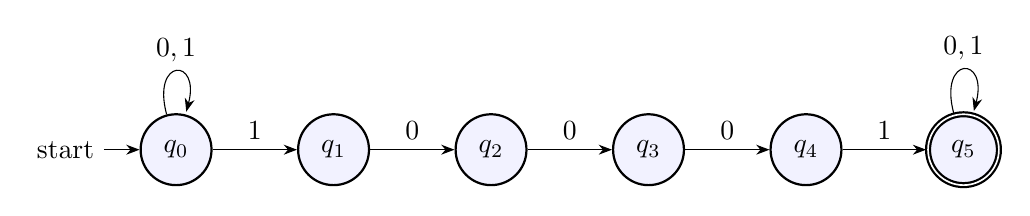
\begin{tikzpicture}[node distance=2cm, on grid, >=Stealth,
    every state/.style={thick, fill=blue!5, minimum size=0.9cm}]
    % States
    \node[state, initial]                (q0) {$q_0$};
    \node[state, right=of q0]           (q1) {$q_1$};
    \node[state, right=of q1]           (q2) {$q_2$};
    \node[state, right=of q2]           (q3) {$q_3$};
    \node[state, right=of q3]           (q4) {$q_4$};
    \node[state, accepting, right=of q4](q5) {$q_5$};

    % Transitions
    \path[->]
      (q0) edge [loop above] node {$0,1$} ()
      (q0) edge              node [above] {$1$}   (q1)
      (q1) edge              node [above] {$0$}   (q2)
      (q2) edge              node [above] {$0$}   (q3)
      (q3) edge              node [above] {$0$}   (q4)
      (q4) edge              node [above] {$1$}   (q5)
      (q5) edge [loop above] node {$0,1$} ();
\end{tikzpicture}
\end{center}

\textbf{How to read this diagram:}
\begin{itemize}[nosep]
\item $q_0$ is the start state (arrow from nowhere). It has a self-loop on both
  $0$ and $1$ --- meaning it can stay in $q_0$ reading anything, waiting to
  ``guess'' that the substring starts now.
\item At any point while in $q_0$ and reading a $1$, the NFA can
  \textbf{nondeterministically} choose to either stay in $q_0$ (via the
  self-loop) \textbf{or} move to $q_1$ (beginning verification).
\item From $q_1$, the path is deterministic: must read $0$, then $0$, then $0$,
  then $1$, matching the substring $10001$.
\item $q_5$ is the accepting state (double circle) with a self-loop --- once
  you've verified the substring, you accept regardless of what comes after.
\item If the NFA guesses wrong (e.g., moves to $q_1$ but the next character
  isn't $0$), that branch ``dies'' --- there's no transition, so it gets stuck.
  But other branches (the ones that stayed in $q_0$) continue.
\end{itemize}

\kt{NFA acceptance = there EXISTS a path from start to accept. The NTM will work
the same way, but with a tape instead of just states.}
\end{examplebox}

%───────────────────────────────────────────────────────────────────────────────
\subsection{NTM Formal Definition (slides 32--33)}
\label{subsec:ntm-formal-def}
%───────────────────────────────────────────────────────────────────────────────

\begin{notebox}{Analogy --- GPS Showing All Routes}
Imagine a GPS navigation app. A normal GPS picks the ``best'' route and shows
you \textbf{one} path from A to B. That's deterministic --- one input (your
location and destination), one output (a single route).

Now imagine a magical GPS that shows you \textbf{every possible route}
simultaneously --- every combination of streets, highways, and shortcuts, all
overlaid on the map at once. You can see all of them. If \emph{any single route}
reaches the destination, the GPS says ``route found!''

This magical GPS is a nondeterministic Turing machine. At every intersection
(configuration with multiple transition options), it takes \emph{all} possible
turns. Each route is a branch. If any branch reaches the destination (state
$t$), the machine accepts.

\textbf{In our formal world:}
\begin{itemize}[nosep]
\item GPS app = the NTM $M$
\item Your location = the current configuration $\gamma$
\item Intersection with multiple options = a configuration where
  $|\delta(q, a)| > 1$
\item Each route on the map = one branch of the computation tree
\item Destination reached = the branch reaches state $t$
\item ``Route found!'' = the NTM accepts
\end{itemize}
\end{notebox}

\begin{definitionbox}{Nondeterministic Turing Machine (NTM)}

\textbf{Plain English:}
A nondeterministic Turing machine is exactly like a deterministic Turing
machine, except for one change: when the machine is in some state $q$ reading
some symbol $a$, instead of having exactly one thing it \emph{must} do, it has
a \textbf{set} of things it \emph{could} do. It ``does all of them at once''
(conceptually). If any one of those parallel computations reaches the accept
state, the machine accepts.

\textbf{Formal Definition:}

An NTM is a 7-tuple:
\fitmath{M = (Q,\; \Sigma,\; \Gamma,\; s,\; t,\; r,\; \delta)}

where all components are the same as a DTM, \textbf{except} the transition
function:

\fitmath{\delta \colon (Q \setminus \{t, r\}) \times \Gamma \;\to\; 2^{Q \times \Gamma \times \{-1, +1\}}}

\textbf{Breaking Down the Notation:}
\begin{itemize}[nosep]
\item $Q$ = finite set of states (same as DTM)
\item $\Sigma$ = input alphabet (same as DTM)
\item $\Gamma$ = tape alphabet with $\Sigma \cup \{\sqcup\} \subseteq \Gamma$
  (same as DTM)
\item $s \in Q$ = start state (same as DTM)
\item $t \in Q$ = accept state (same as DTM)
\item $r \in Q$ = reject state, $r \neq t$ (same as DTM)
\item $\delta$ = the transition function --- \textbf{this is the ONLY difference}:
  \begin{itemize}[nosep]
  \item \textbf{Domain:} $(Q \setminus \{t, r\}) \times \Gamma$ --- same as DTM.
    In non-halting state $q$, reading tape symbol $a$.
  \item \textbf{Codomain:} $2^{Q \times \Gamma \times \{-1, +1\}}$ --- the
    \textbf{power set} of $Q \times \Gamma \times \{-1, +1\}$.
  \item $2^S$ means ``the set of all subsets of $S$.'' So $\delta(q, a)$ returns
    a \textbf{set} of (state, symbol, direction) triples, not just one triple.
  \end{itemize}
\end{itemize}

\textbf{What this means concretely.} Suppose:
\fitmath{\delta(q, a) = \{(q_1, b_1, +1),\; (q_2, b_2, -1)\}}

Then from the configuration where the machine is in state $q$ reading $a$,
there are \textbf{two} possible next configurations:
\begin{enumerate}[nosep]
\item Go to state $q_1$, write $b_1$, move right.
\item Go to state $q_2$, write $b_2$, move left.
\end{enumerate}
The NTM ``takes both'' --- it branches into two parallel computations.

If $\delta(q, a) = \{(q_1, b_1, +1)\}$ (a set with one element), then there is
no choice --- exactly one next configuration. This is the deterministic case.

\kt{A DTM is a special case of an NTM where $|\delta(q,a)| = 1$ for every
$(q,a)$ pair. Every DTM is already an NTM that just never branches.}
\end{definitionbox}

\begin{examplebox}{DTM vs.\ NTM --- Side-by-Side Comparison}
\begin{center}
\renewcommand{\arraystretch}{1.5}
\begin{tabular}{p{3.5cm}p{5.5cm}p{5.5cm}}
\toprule
& \textbf{DTM} & \textbf{NTM} \\
\midrule
\textbf{Transition function} &
  $\delta \colon (Q \setminus \{t,r\}) \times \Gamma \to Q \times \Gamma \times \{-1,+1\}$ &
  $\delta \colon (Q \setminus \{t,r\}) \times \Gamma \to 2^{Q \times \Gamma \times \{-1,+1\}}$ \\
\textbf{Returns} &
  Exactly one triple $(q', b, d)$ &
  A set of triples $\{(q_1, b_1, d_1), \ldots\}$ \\
\textbf{Successor configs} &
  Exactly 1 &
  0, 1, 2, 3, \ldots\ (could be many) \\
\textbf{Computation shape} &
  A \textbf{line} (sequence of configs) &
  A \textbf{tree} (branching at nondeterministic steps) \\
\textbf{Acceptance} &
  The single computation reaches $t$ &
  $\exists$ at least one branch reaching $t$ \\
\textbf{Rejection} &
  The single computation reaches $r$ or loops forever &
  ALL branches reach $r$ or loop (none reaches $t$) \\
\bottomrule
\end{tabular}
\end{center}

\kt{The ONLY difference between a DTM and an NTM is that $\delta$ returns a set
instead of a single element. Everything else --- states, tape, alphabet ---
is identical.}
\end{examplebox}

%───────────────────────────────────────────────────────────────────────────────
\subsection{The Computation Tree (slides 34--35)}
\label{subsec:computation-tree}
%───────────────────────────────────────────────────────────────────────────────

\begin{notebox}{Analogy --- Choose Your Own Adventure Book}
Remember ``Choose Your Own Adventure'' books? You start on page 1. At the
bottom of each page, you make a choice: ``If you open the door, turn to
page 47. If you climb the window, turn to page 23. If you run away, turn to
page 89.''

Each choice leads to a different storyline. Some storylines end with ``You
Win!'' (accepting). Some end with ``You Lose!'' (rejecting). Some go on
forever because you're stuck in a loop of pages that keep pointing to each
other (infinite loop).

A deterministic reader follows \textbf{one} storyline. A nondeterministic
reader follows \textbf{all} storylines simultaneously. If \emph{any} storyline
says ``You Win!'' --- you win.

The full collection of all possible storylines, organized by which choices
lead where, forms a \textbf{tree}. That's the computation tree.

\textbf{In our formal world:}
\begin{itemize}[nosep]
\item Page 1 = the initial configuration $\alpha_w$ (state $s$, input $w$ on
  tape, head at position 0)
\item A choice at the bottom of a page = a nondeterministic branch where
  $|\delta(q, a)| > 1$
\item Each storyline = one root-to-leaf path in the computation tree
\item ``You Win!'' ending = a leaf node in state $t$ (accept)
\item ``You Lose!'' ending = a leaf node in state $r$ (reject)
\item Infinite story (stuck in a loop) = an infinite branch (no leaf)
\end{itemize}
\end{notebox}

\begin{definitionbox}{Computation Tree of an NTM}

\textbf{Plain English:}
The computation tree is a picture of \emph{everything} that can happen when an
NTM $M$ runs on input $w$. The root is the starting configuration. Each node is
a configuration. The children of a node are all the configurations that the NTM
could transition to from that node (one child per element of $\delta(q, a)$).

\textbf{Formal Definition:}
Given NTM $M$ and input $w$, the \textbf{computation tree} $T_M(w)$ is:
\begin{itemize}[nosep]
\item \textbf{Root:} the initial configuration $\alpha_w$
\item \textbf{Children of node $\gamma$:} for configuration $\gamma$ in state
  $q$ reading symbol $a$, the children are all configurations reachable via one
  step --- one child for each $(q', b, d) \in \delta(q, a)$
\item \textbf{Leaves:} configurations in state $t$ (accept) or state $r$
  (reject) --- these have no children because $\delta$ is undefined for $t$
  and $r$
\item \textbf{Infinite branches:} if a path never reaches $t$ or $r$, it
  continues forever (the branch has no leaf)
\end{itemize}

\textbf{Key properties:}
\begin{enumerate}[nosep]
\item The tree may be \textbf{infinite} --- either because branches are infinite
  (loops) or because the branching creates an infinite number of nodes.
\item The \textbf{branching factor} at any node is bounded by $|\delta(q, a)|$
  --- the number of options in the transition set. If the maximum over all
  $(q, a)$ pairs is $b$, then each node has at most $b$ children.
\item \textbf{Branches are independent.} What happens on one branch has
  absolutely no effect on any other branch. Each branch is its own separate
  computation with its own copy of the tape.
\end{enumerate}
\end{definitionbox}

Now let's draw a \textbf{concrete} computation tree. We'll use the NTM for
``contains 110'' (which we'll construct in detail in Section~5.8) running on
input \texttt{0110}. For now, here is the key idea: the machine scans left to
right, and at every $1$ it reads, it can either (a)~keep scanning or (b)~start
verifying that ``110'' appears starting here. Option (b) commits it to checking
the next two symbols.

\begin{examplebox}{Computation Tree: NTM for ``contains 110'' on input 0110}

The NTM has states $\{s, q_1, q_{11}, t, r\}$. We show the full tree. Each
node shows (state, tape, head position). Tape positions are 0-indexed;
$\sqcup$ is blank. We underline the character under the head.

\textbf{Level 0 (root):}

The initial configuration. State $s$, tape = $0110\sqcup$, head at position 0.

\textbf{Level 1:}

In state $s$ reading $0$: $\delta(s, 0) = \{(s, 0, +1)\}$. Only one option: stay in $s$, move right. \textbf{No branching.}

\textbf{Level 2:}

Now in state $s$ at position 1, reading $1$: $\delta(s, 1) = \{(s, 1, +1),\;
(q_1, 1, +1)\}$. \textbf{Two options --- the tree branches!}

\textbf{Levels 3--4:} Each branch continues until it hits $t$ or $r$.

Here is the full tree:

\begin{center}
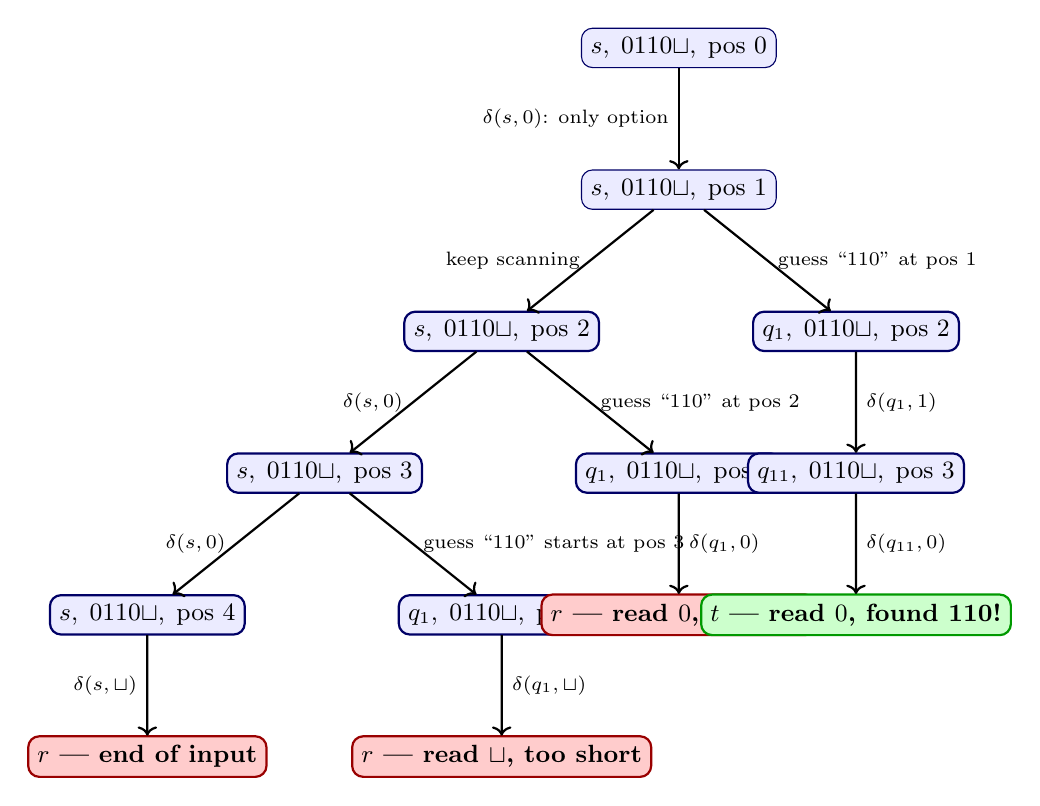
\begin{tikzpicture}[
    level distance=1.8cm,
    sibling distance=4.5cm,
    edge from parent/.style={draw, ->, thick},
    every node/.style={font=\small},
    acc/.style={fill=green!20, draw=green!60!black, rounded corners, font=\small\bfseries},
    rej/.style={fill=red!20, draw=red!60!black, rounded corners, font=\small\bfseries},
    cfg/.style={fill=blue!8, draw=blue!40!black, rounded corners, font=\small},
  ]
  \node[cfg] {$s,\; 0110\sqcup,\; \text{pos } 0$}
    child {
      node[cfg] {$s,\; 0110\sqcup,\; \text{pos } 1$}
        child {
          node[cfg] {$s,\; 0110\sqcup,\; \text{pos } 2$}
            child {
              node[cfg] {$s,\; 0110\sqcup,\; \text{pos } 3$}
                child {
                  node[cfg] {$s,\; 0110\sqcup,\; \text{pos } 4$}
                    child {
                      node[rej] {$r$ --- end of input}
                      edge from parent node[left, font=\scriptsize] {$\delta(s, \sqcup)$}
                    }
                  edge from parent node[left, font=\scriptsize] {$\delta(s, 0)$}
                }
                child {
                  node[cfg] {$q_1,\; 0110\sqcup,\; \text{pos } 4$}
                    child {
                      node[rej] {$r$ --- read $\sqcup$, too short}
                      edge from parent node[right, font=\scriptsize] {$\delta(q_1, \sqcup)$}
                    }
                  edge from parent node[right, font=\scriptsize] {guess ``110'' starts at pos 3}
                }
              edge from parent node[left, font=\scriptsize] {$\delta(s, 0)$}
            }
            child {
              node[cfg] {$q_1,\; 0110\sqcup,\; \text{pos } 3$}
                child {
                  node[rej] {$r$ --- read $0$, not ``1''}
                  edge from parent node[right, font=\scriptsize] {$\delta(q_1, 0)$}
                }
              edge from parent node[right, font=\scriptsize] {guess ``110'' at pos 2}
            }
          edge from parent node[left, font=\scriptsize] {keep scanning}
        }
        child {
          node[cfg] {$q_1,\; 0110\sqcup,\; \text{pos } 2$}
            child {
              node[cfg] {$q_{11},\; 0110\sqcup,\; \text{pos } 3$}
                child {
                  node[acc] {$t$ --- read $0$, found 110!}
                  edge from parent node[right, font=\scriptsize] {$\delta(q_{11}, 0)$}
                }
              edge from parent node[right, font=\scriptsize] {$\delta(q_1, 1)$}
            }
          edge from parent node[right, font=\scriptsize] {guess ``110'' at pos 1}
        }
      edge from parent node[left, font=\scriptsize] {$\delta(s, 0)$: only option}
    };
\end{tikzpicture}
\end{center}

\textbf{Reading the tree:}
\begin{itemize}[nosep]
\item The root is the initial configuration. The machine reads $0$ in state $s$
  --- only one option, so no branching at level 0$\to$1.
\item At position 1, the machine reads $1$ in state $s$. \textbf{Two options:}
  keep scanning (stay in $s$) or guess that ``110'' starts here (go to $q_1$).
  The tree branches.
\item \textbf{Right branch} (guess at position 1): moves to $q_1$, reads $1$ at
  position 2 (good --- second ``1'' found, go to $q_{11}$), reads $0$ at
  position 3 (good --- found ``110''!). \textbf{Reaches state $t$.}
  \textcolor{green!60!black}{\textbf{ACCEPT.}}
\item \textbf{Left branch} continues scanning. At position 2, reads $1$ ---
  branches again. At position 3, reads $0$ --- branches again. Various
  sub-branches try to verify ``110'' starting at positions 2 and 3, but those
  guesses are wrong (position 2: next char is $0$, not $1$; position 3: next
  char is $\sqcup$, too short). They all reach $r$.
\item The leftmost branch scans all the way to the blank and rejects.
\end{itemize}

\textbf{Result:} At least one branch (the right branch from position 1) reaches
$t$. Therefore, the NTM \textbf{accepts} $0110$.

\kt{The computation tree for NTM on $0110$ has one accepting leaf (green) and
several rejecting leaves (red). Since at least one path reaches $t$, the NTM
accepts. This is the ``exists'' rule in action.}
\end{examplebox}

%───────────────────────────────────────────────────────────────────────────────
\subsection{NTM Acceptance: The ``Exists'' Rule (slides 36--37)}
\label{subsec:ntm-acceptance}
%───────────────────────────────────────────────────────────────────────────────

\begin{notebox}{Analogy --- University Applications}
You apply to 10 universities. You get accepted by 3, rejected by 5, and
2 never respond (they ``loop'' forever in their admissions process). The
question: \textbf{are you accepted to university?}

\textbf{YES.} You got into 3 schools. That's enough. The 5 rejections and the
2 non-responses don't cancel out the 3 acceptances. You're going to university.
One acceptance is all you need.

\textbf{In our formal world:}
\begin{itemize}[nosep]
\item 10 universities = 10 branches of the NTM's computation tree
\item 3 accepted = 3 branches reach state $t$
\item 5 rejected = 5 branches reach state $r$
\item 2 never respond = 2 branches loop forever (infinite branches)
\item ``You're accepted!'' = the NTM accepts $w$
\end{itemize}

Now consider a different scenario: you apply to 10 universities. 7 reject you,
3 never respond. \textbf{Are you accepted?} NO --- no one said yes. The fact
that 3 are still ``thinking'' doesn't help. You don't have an acceptance letter.
\end{notebox}

\begin{definitionbox}{NTM Acceptance and Language Recognition}

\textbf{Plain English:}
An NTM accepts a word $w$ if there is \emph{at least one} way the computation
can reach the accept state $t$. It doesn't matter if other branches reject or
loop forever. One success is enough.

\textbf{Formal Definition:}
\begin{itemize}[nosep]
\item $M$ \textbf{accepts} $w$ if $\exists$ a computation of $M$ on $w$ that
  halts in state $t$.
\item $M$ \textbf{does not accept} $w$ if no computation of $M$ on $w$ halts
  in $t$.
  (Every branch either reaches $r$ or loops forever.)
\item The \textbf{language recognized by $M$}:
  \fitmath{L(M) = \{w \in \Sigma^* \mid M \text{ accepts } w\} = \{w \in \Sigma^* \mid \exists \text{ computation of } M \text{ on } w \text{ halting in } t\}}
\end{itemize}

\textbf{Breaking Down the Key Points:}
\begin{itemize}[nosep]
\item \textbf{``$\exists$ a computation''} --- existential quantifier. Not ``for
  all,'' not ``most,'' not ``with high probability'' --- just \textbf{at least
  one}.
\item \textbf{``Does not accept'' is NOT the same as ``rejects.''} An NTM does
  not accept $w$ if no branch reaches $t$. This could be because all branches
  reach $r$ (reject), OR because some branches loop forever and the rest reach
  $r$. Either way: no branch hits $t$, so the word is not accepted.
\item \textbf{Accepts vs.\ rejects vs.\ loops:} Consider an NTM on input $w$:
  \begin{itemize}[nosep]
  \item If some branch reaches $t$ $\Rightarrow$ \textbf{accepts} (regardless
    of other branches)
  \item If all branches reach $r$ $\Rightarrow$ \textbf{rejects}
  \item If no branch reaches $t$, but some branches loop $\Rightarrow$
    \textbf{does not accept} (and we can't definitively say ``reject'' because
    the machine doesn't halt on all branches)
  \end{itemize}
\end{itemize}

\kt{NTM acceptance = $\exists$ (there exists) a branch reaching $t$.
NTM non-acceptance = $\forall$ (for all) branches, none reaches $t$.}
\end{definitionbox}

To make this concrete, let's look at all the possible scenarios:

\begin{examplebox}{All Possible Scenarios for NTM on Input $w$}

Imagine an NTM with 4 branches on some input $w$. Here are all the interesting
combinations:

\begin{center}
\renewcommand{\arraystretch}{1.4}
\begin{tabular}{cccccc}
\toprule
\textbf{Scenario} & \textbf{Branch 1} & \textbf{Branch 2} & \textbf{Branch 3}
& \textbf{Branch 4} & \textbf{NTM result} \\
\midrule
A & $t$ & $r$ & $r$ & $r$ & \textbf{Accepts} \\
B & $t$ & $t$ & $r$ & loops & \textbf{Accepts} \\
C & $t$ & $t$ & $t$ & $t$ & \textbf{Accepts} \\
D & $r$ & $r$ & $r$ & $r$ & \textbf{Does not accept} \\
E & $r$ & $r$ & loops & loops & \textbf{Does not accept} \\
F & loops & loops & loops & loops & \textbf{Does not accept} \\
\bottomrule
\end{tabular}
\end{center}

\textbf{Key observations:}
\begin{itemize}[nosep]
\item Scenarios A, B, C: at least one branch reaches $t$ $\Rightarrow$ accepts.
  It doesn't matter that other branches reject or loop.
\item Scenario D: all branches reject $\Rightarrow$ does not accept (and we can
  also say the machine ``rejects,'' since every branch halted in $r$).
\item Scenario E: some reject, some loop $\Rightarrow$ does not accept. But
  the machine doesn't cleanly ``reject'' either, because it hasn't halted on
  all branches. It just\ldots\ never finishes, partially.
\item Scenario F: all branches loop $\Rightarrow$ does not accept.
\end{itemize}
\end{examplebox}

%───────────────────────────────────────────────────────────────────────────────
\subsection{Exercise 3: The Five Wrong Definitions (slides 37--38)}
\label{subsec:five-wrong-defs}
%───────────────────────────────────────────────────────────────────────────────

The lecture presents five candidate definitions for ``$M$ accepts $w$'' and asks
which are correct. This is a classic exam-style question that tests whether you
\emph{really} understand the ``$\exists$'' in NTM acceptance.

\begin{conceptbox}{Exercise 3 --- Five Candidate Definitions for NTM Acceptance}
Consider an NTM $M$ and input $w$. Which of the following correctly defines
``$M$ accepts $w$''?

\begin{center}
\renewcommand{\arraystretch}{1.6}
\begin{tabular}{clcc}
\toprule
\textbf{\#} & \textbf{Statement} & \textbf{Verdict} & \textbf{Correct?} \\
\midrule
1 & More than one computation halts in $t$ & WRONG & \textcolor{red!70!black}{$\boldsymbol{\times}$} \\
2 & No computation halts in $r$ & WRONG & \textcolor{red!70!black}{$\boldsymbol{\times}$} \\
3 & There exists a computation halting in $t$ & RIGHT & \textcolor{green!60!black}{$\boldsymbol{\checkmark}$} \\
4 & Exactly one accepting computation & WRONG & \textcolor{red!70!black}{$\boldsymbol{\times}$} \\
5 & Every computation halts in $t$ & WRONG & \textcolor{red!70!black}{$\boldsymbol{\times}$} \\
\bottomrule
\end{tabular}
\end{center}

Now let's understand \textbf{exactly why} each wrong answer is wrong, with
concrete counterexamples.
\end{conceptbox}

\begin{examplebox}{Why Statement 1 Is Wrong: ``More Than One Computation Halts in $t$''}

\textbf{The statement:} ``$M$ accepts $w$ if more than one computation halts in
$t$.'' This requires $\geq 2$ accepting branches.

\textbf{Why it's wrong:} One accepting branch is enough. The actual definition
only requires $\exists$ (at least one), not $\geq 2$.

\textbf{Counterexample:} Consider an NTM with 5 branches. Exactly 1 reaches
$t$, the other 4 reach $r$.

By the \textbf{real definition}: $M$ accepts $w$ (there exists a computation
halting in $t$ --- namely branch 1).

By \textbf{statement 1}: $M$ does NOT accept $w$ (only one computation halts in
$t$, not ``more than one'').

Statement 1 is \textbf{too strong} --- it demands multiple successes when one is
enough.
\end{examplebox}

\begin{examplebox}{Why Statement 2 Is Wrong: ``No Computation Halts in $r$''}

\textbf{The statement:} ``$M$ accepts $w$ if no computation halts in $r$.''

\textbf{Why it's wrong:} This confuses the \emph{absence of rejection} with
\emph{acceptance}. What if no branch reaches $t$ AND no branch reaches $r$?
That happens when all branches loop forever.

\textbf{Counterexample:} Consider an NTM where \textbf{all} branches loop
forever on input $w$. No branch reaches $t$, no branch reaches $r$.

By the \textbf{real definition}: $M$ does NOT accept $w$ (no computation halts
in $t$).

By \textbf{statement 2}: $M$ accepts $w$ (``no computation halts in $r$'' is
true, since no computation halts at all!).

Statement 2 would incorrectly say looping = accepting. The real definition says
looping = not accepting.
\end{examplebox}

\begin{examplebox}{Why Statement 3 Is Right: ``There Exists a Computation Halting in $t$''}

\textbf{The statement:} ``$M$ accepts $w$ if there exists a computation halting
in $t$.''

\textbf{This IS the definition.} The word ``exists'' ($\exists$) is doing all
the work. At least one branch reaching $t$ is necessary and sufficient.
\begin{itemize}[nosep]
\item If 1 out of 1000 branches reaches $t$: accepts.
\item If 999 out of 1000 branches reach $t$: accepts.
\item If 0 out of 1000 branches reach $t$: does not accept.
\end{itemize}
\end{examplebox}

\begin{examplebox}{Why Statement 4 Is Wrong: ``Exactly One Accepting Computation''}

\textbf{The statement:} ``$M$ accepts $w$ if exactly one computation halts in
$t$.''

\textbf{Why it's wrong:} Having multiple accepting branches is perfectly fine.
The definition says ``at least one,'' not ``exactly one.''

\textbf{Counterexample:} Consider an NTM where \textbf{3} branches reach $t$
and 2 branches reach $r$ on input $w$.

By the \textbf{real definition}: $M$ accepts $w$ (there exists a computation
halting in $t$ --- in fact, three of them).

By \textbf{statement 4}: $M$ does NOT accept $w$ (three computations halt in
$t$, not ``exactly one'').

Statement 4 is wrong in the opposite direction of statement 1 --- it insists on
\emph{exactly} one success, when any positive number of successes should count.
\end{examplebox}

\begin{examplebox}{Why Statement 5 Is Wrong: ``Every Computation Halts in $t$''}

\textbf{The statement:} ``$M$ accepts $w$ if every computation halts in $t$.''

\textbf{Why it's wrong:} This replaces $\exists$ (there exists) with $\forall$
(for all). It requires \emph{unanimous} acceptance --- every branch must accept.
The real definition only needs one.

\textbf{Counterexample:} Consider our ``contains 110'' NTM on input $0110$.
We saw in Section~5.4 that one branch reaches $t$ but several branches reach
$r$ (the ``wrong guesses'').

By the \textbf{real definition}: $M$ accepts $0110$ (there exists a computation
halting in $t$).

By \textbf{statement 5}: $M$ does NOT accept $0110$ (not every computation halts
in $t$ --- most branches reject!).

Statement 5 is \textbf{far too strong}. If we required every branch to accept,
nondeterminism would be useless --- the machine would only accept inputs where
\emph{every} guess works, which defeats the whole purpose of branching.

\kt{The correct definition uses $\exists$ (at least one branch accepts).
Statement 5 uses $\forall$ (all branches must accept). These are completely
different quantifiers, and confusing them is the \#1 mistake with NTMs.}
\end{examplebox}

%───────────────────────────────────────────────────────────────────────────────
\subsection{Halting NTM (slide 39)}
\label{subsec:halting-ntm}
%───────────────────────────────────────────────────────────────────────────────

\begin{notebox}{Analogy --- Adventure Book Where Every Story Ends}
Remember the ``Choose Your Own Adventure'' analogy? Some adventure books are
well-written: every storyline eventually reaches an ending --- either ``You
Win!'' or ``You Lose!'' There are no circular page references that trap you in
an infinite loop.

A \textbf{halting NTM} is like a well-written adventure book: every branch of
the computation tree eventually reaches either $t$ (accept) or $r$ (reject).
No branch goes on forever. The tree is \textbf{finite}.

\textbf{In our formal world:}
\begin{itemize}[nosep]
\item Well-written book = halting NTM
\item Every story ends = every branch of the computation tree is finite
\item No infinite loops = no infinite branches in the tree
\item The whole tree is finite = the computation tree has finitely many nodes
\end{itemize}
\end{notebox}

\begin{definitionbox}{Halting NTM}

\textbf{Plain English:}
A halting NTM is an NTM that always terminates, no matter what input you give
it and no matter which branch you follow. Every single branch of the computation
tree reaches either the accept state $t$ or the reject state $r$ in finitely
many steps.

\textbf{Formal Definition:}
An NTM $M$ is \textbf{halting} if for every input $w \in \Sigma^*$, the
computation tree $T_M(w)$ is \textbf{finite} --- i.e., every branch has finite
length (every branch terminates in $t$ or $r$).

\textbf{Consequence for acceptance:}
\begin{itemize}[nosep]
\item A halting NTM \textbf{accepts} $w$ $\iff$ at least one leaf of $T_M(w)$
  is in state $t$.
\item A halting NTM \textbf{rejects} $w$ $\iff$ ALL leaves of $T_M(w)$ are in
  state $r$.
\end{itemize}

\textbf{Why this matters:}
\begin{itemize}[nosep]
\item For a \emph{general} NTM, ``does not accept'' could mean ``all branches
  reject'' OR ``some branches loop forever but none accepts.'' You can't
  distinguish these from outside.
\item For a \emph{halting} NTM, ``does not accept'' always means ``all branches
  reject.'' There are no loops. So a halting NTM \textbf{decides} its language
  (it always gives a definitive yes/no answer).
\item This mirrors the DTM distinction: a general DTM \emph{recognizes}
  languages (might loop on non-members), while a \emph{halting} DTM
  \emph{decides} languages (always halts).
\end{itemize}

\kt{Halting NTM = all branches terminate. Accepts $\iff$ $\geq 1$ leaf is $t$.
Rejects $\iff$ all leaves are $r$. No ambiguity, no loops.}
\end{definitionbox}

%───────────────────────────────────────────────────────────────────────────────
\subsection{Constructing NTMs: ``Contains 110'' --- The Main Construction (slides 40--42)}
\label{subsec:construct-110}
%───────────────────────────────────────────────────────────────────────────────

This is where we build a complete NTM from scratch. This is the most important
construction in the nondeterminism section, and you need to understand every
detail.

\begin{notebox}{The ``Guess and Verify'' Pattern}
Most NTMs follow a beautiful two-phase strategy:

\textbf{Phase 1 --- Guess:} Nondeterministically ``guess'' some piece of
information. For example, guess \emph{where} a pattern starts, or guess
\emph{what} a certificate looks like.

\textbf{Phase 2 --- Verify:} Deterministically check whether the guess was
correct.

Because the NTM explores all branches simultaneously, it tries \textbf{every
possible guess}. If any guess turns out to be correct (the verification
succeeds), the machine accepts. If no guess works, all branches reject.

\textbf{Analogy --- Multiple Choice Exam Where You Circle ALL Answers:}

Imagine a test where you can circle \textbf{every} answer choice on every
question, and the grader gives you credit if \emph{any} of your circled answers
is correct. That's what an NTM does:
\begin{itemize}[nosep]
\item Circling all answers = branching (trying every guess)
\item The grader checks each circled answer = deterministic verification on
  each branch
\item Getting credit for any correct answer = accepting if $\exists$ branch
  reaching $t$
\end{itemize}

\textbf{In our ``contains 110'' problem:}
\begin{itemize}[nosep]
\item \textbf{Guess:} at which position does ``110'' start?
\item \textbf{Verify:} starting from that position, are the next three
  characters $1$, $1$, $0$?
\end{itemize}

The NTM scans the input left to right. At each position, it
nondeterministically chooses: ``maybe 110 starts here'' (begin verification) or
``not here, keep scanning'' (continue in the scanning state). It tries
\textbf{every starting position simultaneously}.
\end{notebox}

\begin{definitionbox}{{NTM for $L_2 = \{w \in \{0,1\}^* \mid w \text{ contains 110}\}$}}

\textbf{Plain English:}
This NTM scans the input from left to right. While scanning, every time it
reads a $1$, it branches: one branch continues scanning (maybe 110 starts
later), another branch ``commits'' to checking whether 110 starts at this
position. The committed branch needs to see a second $1$ and then a $0$. If it
does, it accepts. If it doesn't, that branch rejects.

\textbf{Formal Definition:}
\fitmath{M = (\{s, q_1, q_{11}, t, r\},\; \{0, 1\},\; \{0, 1, \sqcup\},\; s,\; t,\; r,\; \delta)}

\textbf{Breaking Down the States:}
\begin{itemize}[nosep]
\item $s$ = \textbf{scanning state}. The machine is scanning right, looking for
  a position to ``guess'' that 110 starts.
\item $q_1$ = \textbf{``seen one 1'' state}. The machine has committed to a
  guess and has verified the first character is $1$. Now it needs to see another
  $1$.
\item $q_{11}$ = \textbf{``seen two 1s'' state}. The machine has seen $1, 1$.
  Now it needs to see a $0$ to complete ``110.''
\item $t$ = \textbf{accept}. The substring 110 was found.
\item $r$ = \textbf{reject}. This particular guess was wrong (or input ended
  without a successful guess).
\end{itemize}
\end{definitionbox}

\begin{examplebox}{Complete Transition Table with Explanations}

Here is every entry of $\delta$, with a plain English explanation of \emph{why}
each transition exists:

\begin{center}
\renewcommand{\arraystretch}{1.5}
\begin{tabular}{ccll}
\toprule
\textbf{State} & \textbf{Read} & \textbf{$\delta(\text{state, read})$} &
\textbf{Explanation} \\
\midrule
$s$ & $0$ & $\{(s, 0, +1)\}$ &
  Reading $0$ while scanning. ``110'' can't start with $0$, \\
& & & so just keep scanning right. Only one option. \\
\midrule
$s$ & $1$ & $\{(s, 1, +1),$ &
  Reading $1$ while scanning. \textbf{NONDETERMINISTIC!} \\
& & $\;\;(q_1, 1, +1)\}$ &
  Option 1: keep scanning (stay in $s$, move right). \\
& & &
  Option 2: guess ``110'' starts here (go to $q_1$). \\
\midrule
$s$ & $\sqcup$ & $\{(r, \sqcup, +1)\}$ &
  Reached end of input while still scanning. \\
& & & Never committed to a guess. Reject. \\
\midrule
$q_1$ & $1$ & $\{(q_{11}, 1, +1)\}$ &
  Committed to a guess. Need second $1$. Got it! \\
& & & Move to $q_{11}$ to check for the $0$. \\
\midrule
$q_1$ & $0$ & $\{(r, 0, -1)\}$ &
  Committed to a guess. Need second $1$, but got $0$. \\
& & & Wrong guess. Reject this branch. \\
\midrule
$q_1$ & $\sqcup$ & $\{(r, \sqcup, +1)\}$ &
  Input ended after seeing only one $1$. \\
& & & Too short for ``110.'' Reject. \\
\midrule
$q_{11}$ & $0$ & $\{(t, 0, +1)\}$ &
  Seen ``11'' so far. Now read $0$. That's ``110''! \\
& & & \textbf{ACCEPT!} Go to state $t$. \\
\midrule
$q_{11}$ & $1$ & $\{(r, 1, +1)\}$ &
  Seen ``11'' so far. Need $0$ but got $1$. \\
& & & Wrong guess (it's ``111\ldots,'' not ``110''). Reject. \\
\midrule
$q_{11}$ & $\sqcup$ & $\{(r, \sqcup, +1)\}$ &
  Seen ``11'' but input ended. Too short. \\
& & & No $0$ to complete ``110.'' Reject. \\
\bottomrule
\end{tabular}
\end{center}

\textbf{Key observation:} There is exactly \textbf{one} nondeterministic
transition --- $\delta(s, 1)$. Every other transition has exactly one option
(deterministic). The nondeterminism is ``surgical'' --- it only appears where
we need to make a guess.

\kt{The NTM for ``contains 110'' uses nondeterminism at exactly one point:
when reading $1$ in the scanning state, it branches into ``keep scanning'' vs.\
``start verifying.'' Everything else is deterministic.}
\end{examplebox}

\begin{examplebox}{State Diagram for the ``Contains 110'' NTM}

\begin{center}
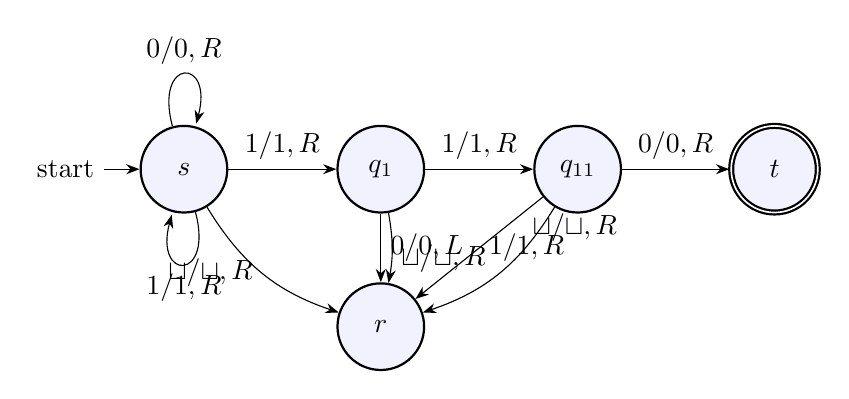
\begin{tikzpicture}[node distance=2.5cm, on grid, >=Stealth,
    every state/.style={thick, fill=blue!5, minimum size=1.1cm}]
    % States
    \node[state, initial]                          (s)   {$s$};
    \node[state, right=of s]                       (q1)  {$q_1$};
    \node[state, right=of q1]                      (q11) {$q_{11}$};
    \node[state, accepting, right=of q11]          (t)   {$t$};
    \node[state, below=2cm of q1]                  (r)   {$r$};

    % Transitions
    \path[->]
      % From s
      (s)   edge [loop above]      node {$0/0,R$}         ()
      (s)   edge [loop below]      node {$1/1,R$}         ()
      (s)   edge                   node [above] {$1/1,R$} (q1)
      (s)   edge [bend right=20]   node [left]  {$\sqcup/\sqcup,R$} (r)
      % From q1
      (q1)  edge                   node [above] {$1/1,R$} (q11)
      (q1)  edge                   node [right] {$0/0,L$} (r)
      (q1)  edge [bend left=10]    node [below right, pos=0.3] {$\sqcup/\sqcup,R$} (r)
      % From q11
      (q11) edge                   node [above] {$0/0,R$} (t)
      (q11) edge                   node [right] {$1/1,R$} (r)
      (q11) edge [bend left=20]    node [above right, pos=0.3] {$\sqcup/\sqcup,R$} (r);
\end{tikzpicture}
\end{center}

\textbf{How to read this diagram:}
\begin{itemize}[nosep]
\item $s$ is the start state (arrow from nowhere). It has \textbf{two}
  transitions on reading $1$: a self-loop (keep scanning) and an arrow to $q_1$
  (start verifying). This is the nondeterministic choice --- shown as two
  separate arrows from the same state on the same input symbol.
\item $s$ has a self-loop on $0$ (keep scanning, no choice to make).
\item From $q_1$, reading $1$ goes to $q_{11}$ (second ``1'' confirmed).
  Reading $0$ or $\sqcup$ goes to $r$ (wrong guess).
\item From $q_{11}$, reading $0$ goes to $t$ (found ``110''! Accept!).
  Reading $1$ or $\sqcup$ goes to $r$ (wrong guess).
\item $t$ is the accept state (double circle). $r$ is the reject state.
\item \textbf{The nondeterminism is visible:} state $s$ has two outgoing arrows
  labeled with the same input symbol $1$. In a DFA/DTM, this would be illegal.
  In an NFA/NTM, it means ``branch.''
\end{itemize}
\end{examplebox}

Now let's trace the NTM's computation on two inputs --- one that should be
accepted and one that should be rejected.

\begin{examplebox}{Full Trace on Input $0110$ --- Should Accept}

Input tape: $\boxed{0}\;\boxed{1}\;\boxed{1}\;\boxed{0}\;\boxed{\sqcup}$
at positions 0, 1, 2, 3, 4.

We trace \textbf{every branch} at \textbf{every step}, showing the state, head
position, and what happens.

\textbf{Step 0:} Configuration $(s, 0110\sqcup, \text{pos}=0)$.
Reading $0$ in state $s$. $\delta(s, 0) = \{(s, 0, +1)\}$. Only one option:
stay in $s$, move right.

\textbf{Step 1:} Configuration $(s, 0110\sqcup, \text{pos}=1)$.
Reading $1$ in state $s$. $\delta(s, 1) = \{(s, 1, +1), (q_1, 1, +1)\}$.
\textbf{BRANCH!} Two successor configurations:
\begin{itemize}[nosep]
\item \textbf{Branch A:} $(s, 0110\sqcup, \text{pos}=2)$ --- kept scanning
\item \textbf{Branch B:} $(q_1, 0110\sqcup, \text{pos}=2)$ --- guessed 110
  starts at pos 1
\end{itemize}

\textbf{Step 2 --- Branch A:} $(s, 0110\sqcup, \text{pos}=2)$.
Reading $1$ in state $s$. Another branch point!
\begin{itemize}[nosep]
\item \textbf{Branch A1:} $(s, 0110\sqcup, \text{pos}=3)$ --- kept scanning
\item \textbf{Branch A2:} $(q_1, 0110\sqcup, \text{pos}=3)$ --- guessed 110
  starts at pos 2
\end{itemize}

\textbf{Step 2 --- Branch B:} $(q_1, 0110\sqcup, \text{pos}=2)$.
Reading $1$ in state $q_1$. $\delta(q_1, 1) = \{(q_{11}, 1, +1)\}$.
One option: go to $q_{11}$, move right.
$\Rightarrow$ $(q_{11}, 0110\sqcup, \text{pos}=3)$

\textbf{Step 3 --- Branch A1:} $(s, 0110\sqcup, \text{pos}=3)$.
Reading $0$ in state $s$. $\delta(s, 0) = \{(s, 0, +1)\}$.
$\Rightarrow$ $(s, 0110\sqcup, \text{pos}=4)$

\textbf{Step 3 --- Branch A2:} $(q_1, 0110\sqcup, \text{pos}=3)$.
Reading $0$ in state $q_1$. $\delta(q_1, 0) = \{(r, 0, -1)\}$.
$\Rightarrow$ \textcolor{red!70!black}{\textbf{REJECT.}} Guessed 110 starts at
pos 2, but position 3 is $0$, not the second $1$ we need.

\textbf{Step 3 --- Branch B:} $(q_{11}, 0110\sqcup, \text{pos}=3)$.
Reading $0$ in state $q_{11}$. $\delta(q_{11}, 0) = \{(t, 0, +1)\}$.
$\Rightarrow$ \textcolor{green!60!black}{\textbf{ACCEPT!}} Guessed 110 starts
at pos 1. Pos 1 = $1$ {\checkmark}, pos 2 = $1$ {\checkmark}, pos 3 = $0$
{\checkmark}. Found ``110''!

\textbf{Step 4 --- Branch A1 continued:} $(s, 0110\sqcup, \text{pos}=4)$.
Reading $\sqcup$ in state $s$. $\delta(s, \sqcup) = \{(r, \sqcup, +1)\}$.
$\Rightarrow$ \textcolor{red!70!black}{\textbf{REJECT.}} Scanned the entire
input without ever committing to a guess.

\textbf{Summary of all branches:}
\begin{center}
\renewcommand{\arraystretch}{1.3}
\begin{tabular}{llc}
\toprule
\textbf{Branch} & \textbf{Description} & \textbf{Result} \\
\midrule
A1 & Scanned everything, never guessed & $r$ (reject) \\
A2 & Guessed 110 starts at pos 2; pos 3 is 0, not 1 & $r$ (reject) \\
B  & Guessed 110 starts at pos 1; verified 1-1-0 & $t$ (\textbf{accept}) \\
\bottomrule
\end{tabular}
\end{center}

At least one branch (B) reaches $t$. Therefore: \textbf{$M$ accepts $0110$.}

\kt{On input $0110$, the NTM tries three guesses. Two are wrong (reject), one
is right (accept). One acceptance is enough: NTM accepts $0110$.}
\end{examplebox}

\begin{examplebox}{Full Trace on Input $0010$ --- Should Reject}

Input tape: $\boxed{0}\;\boxed{0}\;\boxed{1}\;\boxed{0}\;\boxed{\sqcup}$
at positions 0, 1, 2, 3, 4.

This input does NOT contain ``110'' as a substring. The NTM should reject.

\textbf{Step 0:} $(s, 0010\sqcup, \text{pos}=0)$.
Reading $0$ in state $s$. $\delta(s, 0) = \{(s, 0, +1)\}$. No branch.
$\Rightarrow$ $(s, 0010\sqcup, \text{pos}=1)$

\textbf{Step 1:} $(s, 0010\sqcup, \text{pos}=1)$.
Reading $0$ in state $s$. $\delta(s, 0) = \{(s, 0, +1)\}$. No branch.
$\Rightarrow$ $(s, 0010\sqcup, \text{pos}=2)$

\textbf{Step 2:} $(s, 0010\sqcup, \text{pos}=2)$.
Reading $1$ in state $s$. $\delta(s, 1) = \{(s, 1, +1), (q_1, 1, +1)\}$.
\textbf{BRANCH!}
\begin{itemize}[nosep]
\item \textbf{Branch A:} $(s, 0010\sqcup, \text{pos}=3)$ --- kept scanning
\item \textbf{Branch B:} $(q_1, 0010\sqcup, \text{pos}=3)$ --- guessed 110
  starts at pos 2
\end{itemize}

\textbf{Step 3 --- Branch A:} $(s, 0010\sqcup, \text{pos}=3)$.
Reading $0$ in state $s$. No branch.
$\Rightarrow$ $(s, 0010\sqcup, \text{pos}=4)$

\textbf{Step 3 --- Branch B:} $(q_1, 0010\sqcup, \text{pos}=3)$.
Reading $0$ in state $q_1$. $\delta(q_1, 0) = \{(r, 0, -1)\}$.
$\Rightarrow$ \textcolor{red!70!black}{\textbf{REJECT.}} Guessed 110 at pos 2,
but pos 3 is $0$, not the second $1$.

\textbf{Step 4 --- Branch A continued:} $(s, 0010\sqcup, \text{pos}=4)$.
Reading $\sqcup$ in state $s$. $\delta(s, \sqcup) = \{(r, \sqcup, +1)\}$.
$\Rightarrow$ \textcolor{red!70!black}{\textbf{REJECT.}} End of input.

\textbf{Summary of all branches:}
\begin{center}
\renewcommand{\arraystretch}{1.3}
\begin{tabular}{llc}
\toprule
\textbf{Branch} & \textbf{Description} & \textbf{Result} \\
\midrule
A & Scanned everything, never found 110 & $r$ (reject) \\
B & Guessed 110 starts at pos 2; wrong (0 after 1) & $r$ (reject) \\
\bottomrule
\end{tabular}
\end{center}

\textbf{Every} branch reaches $r$. No branch reaches $t$. Therefore:
\textbf{$M$ rejects $0010$.}

This makes sense: $0010$ does not contain ``110'' as a substring. The NTM tried
every possible guess for where ``110'' might start, and every guess failed. No
branch accepted, so the machine rejects.

\kt{On input $0010$, every branch of the NTM rejects. No accepting path exists,
so the NTM rejects $0010$. This is correct: $0010 \notin L_2$.}
\end{examplebox}

%───────────────────────────────────────────────────────────────────────────────
\subsection{Constructing NTMs: Composite Numbers (slide 43)}
\label{subsec:composite}
%───────────────────────────────────────────────────────────────────────────────

\begin{notebox}{Another ``Guess and Verify'' Example}
Let's see the guess-and-verify pattern applied to a different problem to
reinforce the technique. This example appears on the lecture slides.

\textbf{The problem:}
\fitmath{L_{\text{comp}} = \{a^n \mid n \text{ is composite (not prime and } n > 1\text{)}\}}

The input is a string of $n$ copies of the symbol $a$. The NTM should accept if
$n$ is composite (i.e., $n = n_0 \cdot n_1$ for some $n_0, n_1 > 1$).

\textbf{Examples:}
\begin{itemize}[nosep]
\item $a^6 = aaaaaa \in L_{\text{comp}}$ because $6 = 2 \times 3$
\item $a^4 = aaaa \in L_{\text{comp}}$ because $4 = 2 \times 2$
\item $a^5 = aaaaa \notin L_{\text{comp}}$ because 5 is prime
\item $a^1 = a \notin L_{\text{comp}}$ because $1$ is not composite
\end{itemize}
\end{notebox}

\begin{definitionbox}{{NTM for Composite Numbers --- Guess and Verify}}

\textbf{The guess-and-verify strategy:}
\begin{enumerate}[nosep]
\item \textbf{Guess:} Nondeterministically choose two numbers $n_0 > 1$ and
  $n_1 > 1$. (The NTM branches into all possible pairs.)
\item \textbf{Verify:} Deterministically compute $n_0 \cdot n_1$ and check
  whether it equals $n$ (the length of the input). If yes, accept. If no,
  reject.
\end{enumerate}

This is purely conceptual --- we're not writing out the full transition table
(it would be enormous). The point is the \emph{pattern}: guess a certificate,
verify it deterministically.
\end{definitionbox}

\begin{examplebox}{Composite Numbers NTM --- Concrete Traces}

\textbf{Input: $a^6$ (i.e., $aaaaaa$, so $n = 6$).}

The NTM branches into all possible guesses for $(n_0, n_1)$ with
$n_0, n_1 > 1$:

\begin{center}
\renewcommand{\arraystretch}{1.3}
\begin{tabular}{cccc}
\toprule
\textbf{Branch} & \textbf{Guess $(n_0, n_1)$} & \textbf{$n_0 \cdot n_1$} &
\textbf{Result} \\
\midrule
1 & $(2, 2)$ & $4 \neq 6$ & $r$ (reject) \\
2 & $(2, 3)$ & $6 = 6$ & $t$ (\textbf{accept!}) \\
3 & $(2, 4)$ & $8 \neq 6$ & $r$ (reject) \\
4 & $(3, 2)$ & $6 = 6$ & $t$ (\textbf{accept!}) \\
5 & $(3, 3)$ & $9 \neq 6$ & $r$ (reject) \\
\ldots & \ldots & \ldots & \ldots \\
\bottomrule
\end{tabular}
\end{center}

Branches 2 and 4 reach $t$. At least one accepting branch exists.
$\Rightarrow$ \textbf{NTM accepts $a^6$.} Correct: $6$ is composite.

\bigskip

\textbf{Input: $a^5$ (i.e., $aaaaa$, so $n = 5$).}

The NTM branches into all possible guesses:

\begin{center}
\renewcommand{\arraystretch}{1.3}
\begin{tabular}{cccc}
\toprule
\textbf{Branch} & \textbf{Guess $(n_0, n_1)$} & \textbf{$n_0 \cdot n_1$} &
\textbf{Result} \\
\midrule
1 & $(2, 2)$ & $4 \neq 5$ & $r$ (reject) \\
2 & $(2, 3)$ & $6 \neq 5$ & $r$ (reject) \\
3 & $(3, 2)$ & $6 \neq 5$ & $r$ (reject) \\
4 & $(2, 4)$ & $8 \neq 5$ & $r$ (reject) \\
5 & $(4, 2)$ & $8 \neq 5$ & $r$ (reject) \\
\ldots & \ldots & \ldots & $r$ (reject) \\
\bottomrule
\end{tabular}
\end{center}

No pair $(n_0, n_1)$ with $n_0, n_1 > 1$ satisfies $n_0 \cdot n_1 = 5$.
\textbf{Every} branch rejects. $\Rightarrow$ \textbf{NTM rejects $a^5$.}
Correct: $5$ is prime.

\kt{The composite-number NTM perfectly illustrates ``guess and verify'': guess a
factorization, verify it matches. Correct guesses $\Rightarrow$ accept. No
correct guess exists $\Rightarrow$ all branches reject.}
\end{examplebox}

%───────────────────────────────────────────────────────────────────────────────
\subsection{The NTM Simulation Theorem (slides 44--45)}
\label{subsec:ntm-simulation}
%───────────────────────────────────────────────────────────────────────────────

This is the payoff of the entire section. We now prove that nondeterminism does
NOT add computational power: every NTM can be simulated by a DTM. The DTM is
slower, but it recognizes exactly the same language.

\begin{notebox}{Analogy --- Systematic Chess Player vs.\ ``See the Future'' Player}
Imagine two chess players:

\textbf{Player N (the ``future-seer''):} At every move, this player magically
sees \emph{all possible futures} of the game simultaneously. They see every
possible sequence of moves by both players, all playing out at once. If
\emph{any} sequence of moves leads to checkmate, they know it instantly.

\textbf{Player D (the ``systematic thinker''):} This player can't see the
future. Instead, they have a notebook. They systematically write down all
possible moves at depth 1 (``what if I move the pawn? the knight? the
bishop?''). Then they consider all possible responses at depth 2. Then depth 3.
And so on. They check \emph{all} possibilities at depth $d$ before moving to
depth $d+1$.

Player D is slower --- much slower. But they \emph{never miss a winning
sequence}. If there's a checkmate in 5 moves, Player D will find it when they
reach depth 5 in their systematic search. They'll find exactly the same
checkmates that Player N sees.

\textbf{In our formal world:}
\begin{itemize}[nosep]
\item Player N = the NTM (explores all computation branches simultaneously)
\item Player D = the simulating DTM (systematically explores the computation
  tree level by level, i.e., BFS)
\item Depth $d$ in the game tree = level $d$ in the computation tree
\item ``All possible moves at depth 1, then depth 2, \ldots'' = BFS traversal:
  $\Gamma_0$, then $\Gamma_1$, then $\Gamma_2$, \ldots
\item Checkmate found = accepting configuration found (state $t$)
\item ``D finds the same checkmates as N'' = DTM accepts exactly the same
  language as the NTM
\end{itemize}
\end{notebox}

\begin{definitionbox}{{Theorem: Every NTM Can Be Simulated by a DTM}}

\textbf{Plain English:}
For any nondeterministic Turing machine $N$, there exists a deterministic
Turing machine $D$ such that $L(D) = L(N)$. Furthermore, if $N$ is halting
(always terminates on all branches), then $D$ is also halting.

\textbf{Formal Statement:}

For every NTM $N$, there exists a DTM $D$ such that:
\begin{enumerate}[nosep]
\item $L(D) = L(N)$ \quad (they recognize the same language)
\item If $N$ is halting, then $D$ is halting \quad (decidability is preserved)
\end{enumerate}

\textbf{What This Means:}
\begin{itemize}[nosep]
\item \textbf{Computably-enumerable} (c.e.) languages $=$ languages recognized
  by some NTM $=$ languages recognized by some DTM. Adding nondeterminism
  doesn't expand the class.
\item \textbf{Computable} (decidable) languages $=$ languages decided by some
  halting NTM $=$ languages decided by some halting DTM. Same story.
\end{itemize}
\end{definitionbox}

\begin{definitionbox}{{The BFS Simulation Algorithm}}

\textbf{High-level idea:} The DTM simulates the NTM by performing a
\textbf{breadth-first search} (BFS) of the computation tree. It generates all
configurations at level 0, then all at level 1, then level 2, and so on. At
each level, it checks whether any configuration is accepting.

\textbf{Why BFS and not DFS?} We explain this in detail after the algorithm.
Short answer: DFS might go down an infinite branch and never come back. BFS
guarantees we check all branches at every depth.

Here is the algorithm with line-by-line comments:

\begin{lstlisting}[mathescape=true, escapeinside={(*}{*)}]
def simulate_NTM(N, w):                        (*\color{gray}{\% Input: NTM $N$ and word $w$}*)
    $\Gamma_0$ = {initial_config(N, w)}           (*\color{gray}{\% Level 0: just the start config $\alpha_w$}*)
    i = 0                                      (*\color{gray}{\% Current level counter (depth in tree)}*)
    while True:                                (*\color{gray}{\% Keep going until we find an answer}*)
        if $\Gamma_i$ has an accepting config:    (*\color{gray}{\% Check: is any config in state $t$?}*)
            return ACCEPT                      (*\color{gray}{\% Yes! $\exists$ branch accepts $\Rightarrow$ accept}*)
        if $\Gamma_i$ is empty:                   (*\color{gray}{\% Check: did all branches die?}*)
            return REJECT                      (*\color{gray}{\% No configs left $\Rightarrow$ all rejected}*)
        $\Gamma_{i+1}$ = {}                       (*\color{gray}{\% Prepare next level (start empty)}*)
        for each $\gamma$ in $\Gamma_i$:              (*\color{gray}{\% For every config at current level}*)
            for each successor $\gamma'$ of $\gamma$: (*\color{gray}{\% Find all successor configs via $\delta$}*)
                add $\gamma'$ to $\Gamma_{i+1}$       (*\color{gray}{\% Collect into next level}*)
        i = i + 1                              (*\color{gray}{\% Move to next level}*)
\end{lstlisting}

\textbf{Breaking Down the Algorithm:}
\begin{itemize}[nosep]
\item $\Gamma_i$ = the set of \textbf{all configurations reachable in exactly
  $i$ steps} from the initial configuration. This is level $i$ of the
  computation tree.
\item $\Gamma_0 = \{\alpha_w\}$ = just the initial configuration (the root of
  the tree).
\item ``has an accepting config'' = $\exists \gamma \in \Gamma_i$ such that
  $\gamma$ is in state $t$.
\item ``is empty'' = $\Gamma_i = \emptyset$, meaning every branch has already
  terminated (reached $t$ or $r$) at some earlier level, so there are no
  configurations left to explore. This only happens for halting NTMs.
\item ``successor $\gamma'$ of $\gamma$'' = for config $\gamma$ in state $q$
  reading $a$, the successors are all configs reachable via the triples in
  $\delta(q, a)$.
\item The algorithm generates $\Gamma_0, \Gamma_1, \Gamma_2, \ldots$ level by
  level, checking each for an accepting configuration.
\end{itemize}

\textbf{Correctness:}
\begin{itemize}[nosep]
\item If the NTM accepts $w$, then $\exists$ a branch of length $k$ ending in
  $t$. The DTM's BFS will find this accepting configuration in $\Gamma_k$.
  $\Rightarrow$ DTM accepts.
\item If the NTM rejects $w$ (all branches halt in $r$), then eventually all
  branches terminate, $\Gamma_i$ becomes empty, and the DTM returns REJECT.
  $\Rightarrow$ DTM rejects.
\item If the NTM loops on $w$ (some branches loop forever, none reaches $t$),
  then the DTM's BFS also loops forever (keeps generating non-empty $\Gamma_i$
  levels that never contain an accepting config).
  $\Rightarrow$ DTM loops.
\end{itemize}

In all three cases, DTM matches NTM. Therefore $L(D) = L(N)$.
\end{definitionbox}

\begin{examplebox}{BFS Simulation Trace: ``Contains 110'' NTM on Input $0110$}

Let's trace the BFS algorithm step by step. We show $\Gamma_i$ for each level.
Each configuration is written as (state, head position) since the tape doesn't
change (this NTM only reads, never writes anything different).

\textbf{Level 0:} $\Gamma_0 = \{(s, 0)\}$

One configuration. Check for accepting config: $s \neq t$. Not accepting.
$\Gamma_0$ is not empty. Continue.

Generate successors: $(s, 0)$ reading $0$: $\delta(s, 0) = \{(s, 0, +1)\}$.
One successor: $(s, 1)$.

\textbf{Level 1:} $\Gamma_1 = \{(s, 1)\}$

One configuration. $s \neq t$. Not accepting. Not empty. Continue.

Generate successors: $(s, 1)$ reading $1$:
$\delta(s, 1) = \{(s, 1, +1), (q_1, 1, +1)\}$. Two successors: $(s, 2)$ and
$(q_1, 2)$.

\textbf{Level 2:} $\Gamma_2 = \{(s, 2),\; (q_1, 2)\}$

Two configurations. Neither is in state $t$. Not empty. Continue.

Generate successors:
\begin{itemize}[nosep]
\item $(s, 2)$ reading $1$: $\delta(s, 1) = \{(s, 1, +1), (q_1, 1, +1)\}$.
  Successors: $(s, 3)$, $(q_1, 3)$.
\item $(q_1, 2)$ reading $1$: $\delta(q_1, 1) = \{(q_{11}, 1, +1)\}$.
  Successor: $(q_{11}, 3)$.
\end{itemize}

\textbf{Level 3:} $\Gamma_3 = \{(s, 3),\; (q_1, 3),\; (q_{11}, 3)\}$

Three configurations. Check for accepting: $s \neq t$, $q_1 \neq t$,
$q_{11} \neq t$. None accepting. Not empty. Continue.

Generate successors:
\begin{itemize}[nosep]
\item $(s, 3)$ reading $0$: $\delta(s, 0) = \{(s, 0, +1)\}$. Successor:
  $(s, 4)$.
\item $(q_1, 3)$ reading $0$: $\delta(q_1, 0) = \{(r, 0, -1)\}$. Successor:
  $(r, 2)$. This is a halting config (state $r$), so it won't generate
  further successors.
\item $(q_{11}, 3)$ reading $0$: $\delta(q_{11}, 0) = \{(t, 0, +1)\}$.
  Successor: $(t, 4)$.
\end{itemize}

\textbf{Level 4:} $\Gamma_4 = \{(s, 4),\; (r, 2),\; (t, 4)\}$

Three configurations. Check for accepting: $(t, 4)$ is in state $t$!

\textbf{ACCEPTING CONFIG FOUND!} Return \textbf{ACCEPT}.

\begin{center}
\renewcommand{\arraystretch}{1.3}
\begin{tabular}{cll}
\toprule
\textbf{Level} & \textbf{$\Gamma_i$} & \textbf{Accepting?} \\
\midrule
0 & $\{(s, 0)\}$ & No \\
1 & $\{(s, 1)\}$ & No \\
2 & $\{(s, 2),\; (q_1, 2)\}$ & No \\
3 & $\{(s, 3),\; (q_1, 3),\; (q_{11}, 3)\}$ & No \\
4 & $\{(s, 4),\; (r, 2),\; (t, 4)\}$ & \textbf{Yes!} $(t, 4) \in \Gamma_4$ \\
\bottomrule
\end{tabular}
\end{center}

The DTM's BFS found the accepting configuration at level 4. It returns ACCEPT,
matching the NTM's behavior.

\kt{The BFS simulation generates all reachable configurations level by level.
At level 4, it finds $(t, 4)$ --- the accepting config. The DTM accepts $0110$,
just like the NTM does.}
\end{examplebox}

\begin{conceptbox}{{Why BFS, Not DFS? --- This Is Critical}}

\textbf{The problem with DFS (Depth-First Search):}

DFS explores one branch all the way to its end before backtracking to try the
next branch. This is dangerous when branches can be \textbf{infinite}.

\begin{center}
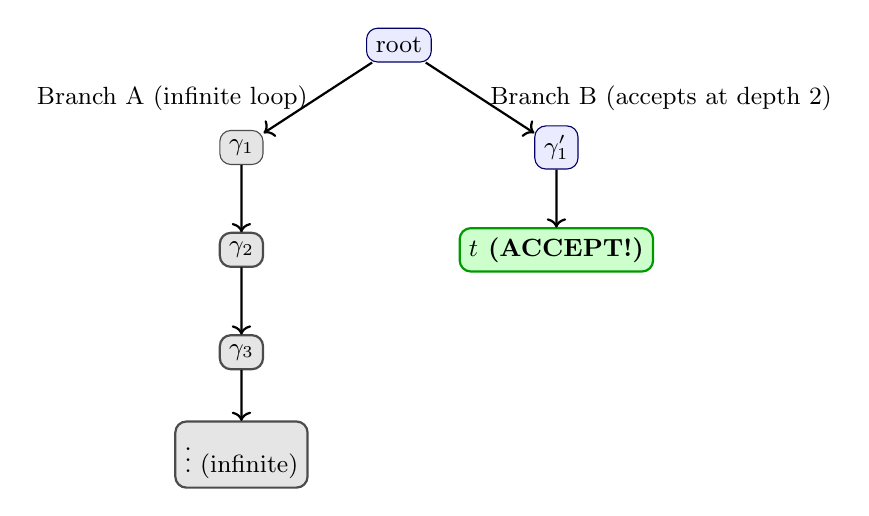
\begin{tikzpicture}[
    level distance=1.3cm,
    sibling distance=4cm,
    edge from parent/.style={draw, ->, thick},
    every node/.style={font=\small},
    acc/.style={fill=green!20, draw=green!60!black, rounded corners,
      font=\small\bfseries},
    inf/.style={fill=gray!20, draw=gray!60!black, rounded corners,
      font=\small},
    cfg/.style={fill=blue!8, draw=blue!40!black, rounded corners,
      font=\small},
  ]
  \node[cfg] {root}
    child {
      node[inf] {$\gamma_1$}
        child {
          node[inf] {$\gamma_2$}
            child {
              node[inf] {$\gamma_3$}
                child {
                  node[inf] {$\vdots$ (infinite)}
                }
            }
        }
      edge from parent node[left] {Branch A (infinite loop)}
    }
    child {
      node[cfg] {$\gamma'_1$}
        child {
          node[acc] {$t$ (ACCEPT!)}
        }
      edge from parent node[right] {Branch B (accepts at depth 2)}
    };
\end{tikzpicture}
\end{center}

\textbf{What DFS does:} It goes down Branch A first. $\gamma_1 \to \gamma_2
\to \gamma_3 \to \gamma_4 \to \ldots$ forever. It \textbf{never comes back} to
try Branch B. The accepting configuration in Branch B at depth 2 is missed.
The DTM loops forever, even though the NTM accepts!

\textbf{What BFS does:}
\begin{itemize}[nosep]
\item Level 0: root. Not accepting. Continue.
\item Level 1: $\{\gamma_1, \gamma'_1\}$. Neither accepting. Continue.
\item Level 2: $\{\gamma_2, t\}$. \textbf{Found $t$!} ACCEPT.
\end{itemize}

BFS finds the accepting config at depth 2. It checks \emph{all} branches at
each depth before going deeper. It can't get ``trapped'' in an infinite branch
because it never goes deeper than level $d$ until it has checked every node at
level $d$.

\textbf{The guarantee:} If there exists an accepting computation of length $k$
(a branch that reaches $t$ in $k$ steps), BFS will find it when it reaches
level $k$. It doesn't matter if other branches are infinite --- BFS processes
level $k$ in finite time (each level has finitely many configurations because
the branching factor is finite).

\kt{BFS is essential because DFS can get trapped in an infinite branch, missing
a short accepting branch. BFS checks ALL branches at depth $d$ before going to
$d+1$, guaranteeing that any finite accepting path is found.}
\end{conceptbox}

\begin{definitionbox}{{Corollaries of the NTM Simulation Theorem}}

The simulation theorem gives us two important equivalences. These are the NTM
versions of the characterizations we already had for DTMs.

\textbf{Corollary 1 (Computably-enumerable languages):}
\fitmath{L \text{ is computably-enumerable} \;\iff\; L = L(N) \text{ for some NTM } N}

\textbf{Plain English:} A language is c.e.\ if and only if some NTM recognizes
it. This is because:
\begin{itemize}[nosep]
\item ($\Leftarrow$): If NTM $N$ recognizes $L$, then by the simulation
  theorem, some DTM $D$ also recognizes $L$. So $L$ is c.e.\ (by the DTM
  definition of c.e.).
\item ($\Rightarrow$): If $L$ is c.e., some DTM recognizes it. Every DTM is
  already an NTM (with $|\delta(q,a)| = 1$ always). So some NTM recognizes $L$.
\end{itemize}

\textbf{Corollary 2 (Computable / decidable languages):}
\fitmath{L \text{ is computable} \;\iff\; L = L(N) \text{ for some halting NTM } N}

\textbf{Plain English:} A language is decidable if and only if some
\emph{halting} NTM decides it. The simulation theorem preserves the halting
property.

\kt{Adding nondeterminism to TMs does not change the classes of c.e.\ or
computable languages. NTMs recognize exactly the same languages as DTMs.
This is the ``same power, different convenience'' story, just like multi-tape.}
\end{definitionbox}
\newpage
%═══════════════════════════════════════════════════════════════════════════════
\section{More Robustness: The Doubly-Infinite Tape (Exercise 2, Tutorial 2)} \kemark
%═══════════════════════════════════════════════════════════════════════════════

This section covers \textbf{Exercise 2 from Tutorial 2}. The exercise has three
parts, and we walk through each one in full detail. By the end, you will have a
fourth robustness result: changing the shape of the tape does not add
computational power.

%───────────────────────────────────────────────────────────────────────────────
\subsection{What Is a Doubly-Infinite Tape?}
\label{subsec:doubly-infinite-what}
%───────────────────────────────────────────────────────────────────────────────

\begin{notebox}{Analogy: Receipt Paper vs.\ a Strip Floating in Space}
Picture a receipt printer at a grocery store. The paper roll has a clear
\textbf{beginning} --- the point where the paper is attached to the roll ---
and it unrolls infinitely to one side (you can always print more). If you try
to pull the paper \emph{backwards} past the attachment point, you can't ---
there's nothing there. That beginning is a hard boundary.

Now imagine you rip the receipt off the roll and let it float in zero gravity
in the middle of a room. There is no ``start'' and no ``end'' anymore. You
can drift to the left as far as you want, or drift to the right as far as you
want. The strip extends infinitely in \emph{both} directions.

\textbf{In our formal world:}
\begin{itemize}[nosep]
\item Receipt paper roll = \textbf{singly-infinite tape} (standard TM). The
  attachment point is cell 1 --- the leftmost cell. Cells are numbered
  $1, 2, 3, \ldots$ The head cannot go left of cell 1.
\item Strip floating in space = \textbf{doubly-infinite tape}. No left wall,
  no right wall. Cells are numbered $\ldots, -2, -1, 0, 1, 2, \ldots$ (all
  integers $\mathbb{Z}$). The head can go left forever.
\item Attachment point = position 1 boundary on a singly-infinite tape.
\item No attachment point = no boundary at all on a doubly-infinite tape.
\end{itemize}
\end{notebox}

\begin{conceptbox}{Why Consider a Doubly-Infinite Tape?}
\textbf{The Core Problem:}

On a standard (singly-infinite) TM, when the head is at position 1 and the
transition says ``move left,'' the head \textbf{stays at position 1}. It gets
``stuck'' against the left wall. This means:
\begin{itemize}[nosep]
\item Every TM algorithm must \emph{remember} that the left boundary exists.
\item Some algorithms require awkward workarounds to avoid running into the
  wall (e.g., placing a special marker at the leftmost cell so you know
  you've reached the edge).
\end{itemize}

On a doubly-infinite tape, you can \textbf{always go left}. The tape extends
infinitely in both directions. Some algorithms become simpler to design when
you don't have to worry about the left boundary.

\textbf{The Question:} Does this convenience add \textbf{computational power}?
Can a doubly-infinite tape TM decide languages that a standard TM cannot?

Spoiler: \textbf{No.} The two models are equivalent. That is exactly what
Exercise 2 asks you to prove, and that is exactly what we will trace through
in this section.

\kt{The doubly-infinite tape removes the left boundary of a standard TM.
The question is whether this makes the machine more powerful --- and the
answer is no. This is our fourth robustness result.}
\end{conceptbox}

%───────────────────────────────────────────────────────────────────────────────
\subsection{Part 1: Formal Definition of a Doubly-Infinite Tape DTM}
\label{subsec:doubly-infinite-formal}
%───────────────────────────────────────────────────────────────────────────────

\begin{notebox}{{Analogy: Same Vending Machine, Different Shelf Layout}}
Think of a vending machine. The \textbf{machine itself} --- its buttons, its
coin slot, its dispensing mechanism --- doesn't change. What changes is the
\textbf{shelf layout inside}: instead of shelves labeled $1, 2, 3, \ldots$
(starting from shelf 1 at the top), you now have shelves labeled
$\ldots, -2, -1, 0, 1, 2, \ldots$ (extending upward and downward
indefinitely). The robot arm that fetches items can now reach shelves in
\emph{both} directions.

\textbf{In our formal world:}
\begin{itemize}[nosep]
\item Vending machine = the TM tuple $(Q, \Sigma, \Gamma, s, t, r, \delta)$
  --- this does NOT change.
\item Shelf layout = the tape and how cells are indexed --- this is what
  changes (from $\mathbb{N}$ to $\mathbb{Z}$).
\item Robot arm = the read/write head --- now it can reach negative-numbered
  cells too.
\end{itemize}
\end{notebox}

\begin{definitionbox}{{Doubly-Infinite Tape DTM --- The Tuple}}
\textbf{Plain English:}
A doubly-infinite tape DTM has \textbf{exactly the same 7-tuple} as a standard
DTM. The states, alphabets, start/accept/reject states, and transition
function are all identical. What changes is not the machine's description but
\textbf{how the machine operates} --- specifically, how we define
configurations and how the head moves.

\textbf{Formal:}
A doubly-infinite tape DTM is a 7-tuple:
\fitmath{M = (Q,\; \Sigma,\; \Gamma,\; s,\; t,\; r,\; \delta)}
with exactly the same meaning as for a standard DTM:
\begin{itemize}[nosep]
\item $Q$ = finite set of states
\item $\Sigma$ = input alphabet (no blank symbol)
\item $\Gamma \supseteq \Sigma \cup \{\sqcup\}$ = tape alphabet
\item $s \in Q$ = start state
\item $t \in Q$ = accept state
\item $r \in Q$, $r \neq t$ = reject state
\item $\delta \colon (Q \setminus \{t,r\}) \times \Gamma \to Q \times \Gamma \times \{-1,+1\}$ = transition function
\end{itemize}

The transition function is identical: read a symbol, write a symbol, move left
($-1$) or right ($+1$). Nothing in the tuple changes.

\textbf{What changes is the SEMANTICS} --- the meaning of ``configuration''
and ``successor configuration.'' That's in the next box.
\end{definitionbox}

\begin{definitionbox}{{Doubly-Infinite Tape DTM --- Configurations}}
\textbf{Plain English:}
A configuration is a snapshot of the machine at one moment in time: what state
it's in, what's on the tape, and where the head is. For a doubly-infinite
tape, the tape content is a function from \emph{all integers} (not just
positive integers) to tape symbols. The head position can be any integer,
including negative numbers.

\textbf{Formal:}
A \textbf{configuration} is a triple $[q, \tau, \ell]$ where:
\begin{itemize}[nosep]
\item $q \in Q$ is the current state
\item $\tau \colon \mathbb{Z} \to \Gamma$ is the tape content
\item $\ell \in \mathbb{Z}$ is the head position
\end{itemize}

\textbf{Breaking Down the Notation:}
\begin{itemize}[nosep]
\item $\mathbb{Z}$ means \textbf{all integers}: $\ldots, -3, -2, -1, 0, 1, 2, 3, \ldots$ This is the key difference from a standard TM, where the tape is indexed by $\mathbb{N} = \{1, 2, 3, \ldots\}$.
\item $\tau \colon \mathbb{Z} \to \Gamma$ means every integer position maps to some tape symbol. Position $-5$ has a symbol, position $0$ has a symbol, position $42$ has a symbol.
\item $\ell \in \mathbb{Z}$ means the head can be at position $-3$, or $0$, or $17$ --- any integer at all, including negative ones. On a standard TM, the head position is always $\geq 1$.
\end{itemize}

\textbf{Initial configuration} on input $w = w_1 w_2 \cdots w_k$:
\fitmath{[s,\; \tau_0,\; 1]}
where:
\fitmath{\tau_0(n) = \begin{cases} w_n & \text{if } n \in \{1, \ldots, k\} \\ \sqcup & \text{otherwise (including } n = 0, -1, -2, \ldots\text{)} \end{cases}}

\textbf{In words:} The input is placed at positions $1$ through $k$ (just
like a standard TM). Every other cell --- including all the negative
positions and zero --- contains the blank symbol $\sqcup$. The head starts at
position 1, in the start state $s$.
\end{definitionbox}

\begin{definitionbox}{{Doubly-Infinite Tape DTM --- Successor Configuration}}
\textbf{Plain English:}
Given a configuration $[q, \tau, \ell]$, the machine reads the symbol at the
head position, looks up the transition, writes a new symbol, changes state,
and moves the head. This is exactly the same as a standard TM --- with one
critical difference: there is \textbf{no special case} for the head being at
the leftmost cell.

\textbf{Formal:}
If $\delta(q, \tau(\ell)) = (p, a, d)$ where $d \in \{-1, +1\}$, then the
successor configuration is:
\fitmath{[p,\; \tau',\; \ell + d]}
where:
\fitmath{\tau'(n) = \begin{cases} a & \text{if } n = \ell \\ \tau(n) & \text{otherwise} \end{cases}}

\textbf{Breaking Down the Notation:}
\begin{itemize}[nosep]
\item $\tau(\ell)$ = the symbol currently under the head (at position $\ell$)
\item $(p, a, d)$ = the transition's output: go to state $p$, write symbol
  $a$, move in direction $d$
\item $\tau'$ = the updated tape: identical to $\tau$ everywhere except at
  position $\ell$, where the old symbol is replaced by $a$
\item $\ell + d$ = the new head position. If $d = +1$, head moves right. If
  $d = -1$, head moves left.
\end{itemize}

\textbf{THE KEY DIFFERENCE from a standard TM:}

On a standard singly-infinite tape, the successor rule has a special case:
\begin{quote}
``If $\ell = 1$ and $d = -1$, the head stays at position 1 (cannot go left
of the boundary).''
\end{quote}

On a doubly-infinite tape, \textbf{this special case does not exist}. If the
head is at position 1 and the transition says ``move left,'' the head goes to
position \textbf{0}. If the head is at position 0 and says ``move left,'' it
goes to position $-1$. The head can always go left, without limit.

\textbf{Accepting, rejecting, and halting:} Same as standard DTM. The machine
accepts when it enters state $t$, rejects when it enters state $r$, and halts
when it enters either.
\end{definitionbox}

\begin{examplebox}{Concrete Example: Input ``01'' on a Doubly-Infinite Tape}
Let's see exactly what the tape looks like for input $w = 01$ (so $k = 2$,
$w_1 = 0$, $w_2 = 1$).

\textbf{Initial configuration:} $[s, \tau_0, 1]$

The tape content $\tau_0$ assigns symbols to every integer:
\begin{center}
\begin{tabular}{c|cccccccc}
Position & $\cdots$ & $-2$ & $-1$ & $0$ & $1$ & $2$ & $3$ & $\cdots$ \\
\hline
Symbol & $\cdots$ & $\sqcup$ & $\sqcup$ & $\sqcup$ & $\mathtt{0}$ & $\mathtt{1}$ & $\sqcup$ & $\cdots$ \\
\end{tabular}
\end{center}

The head is at position 1 (pointing at the $\mathtt{0}$). All positions outside
$\{1, 2\}$ contain blanks --- including position 0, $-1$, $-2$, and so on.

\textbf{What happens if the head moves left from position 1?}

On a \textbf{standard TM}: the head stays at position 1 (stuck against the
left wall).

On a \textbf{doubly-infinite tape TM}: the head moves to position 0. It reads
$\sqcup$ (blank) there. If it moves left again, it goes to position $-1$ ---
also blank. There is no wall. The head just keeps finding blank cells as it
moves further left.

\kt{The only difference between a singly-infinite and doubly-infinite tape DTM
is in the successor configuration: no left boundary means the head can always
move left, finding blank cells extending infinitely to the left.}
\end{examplebox}


%───────────────────────────────────────────────────────────────────────────────
\subsection{Part 2: Singly-Infinite Simulates Doubly-Infinite (The Hard Direction)}
\label{subsec:singly-simulates-doubly}
%───────────────────────────────────────────────────────────────────────────────

This is the hard direction. A singly-infinite tape has positions $1, 2, 3,
\ldots$ but a doubly-infinite tape needs $\ldots, -2, -1, 0, 1, 2, \ldots$
How do you fit an infinite-in-both-directions tape onto a tape that only goes
one way?

\begin{notebox}{Analogy: Fitting a Two-Way Street onto a One-Way Street}
Imagine you have a street that goes in \textbf{both directions} --- cars drive
east and west. Now the city needs to convert it into a \textbf{one-way street}
(only east). But you still need to handle all the traffic that used to go
west.

The solution: put up \textbf{barriers} at the beginning and end of the active
zone. Whenever a car needs to go west past the barrier, you \textbf{shift} all
the parked cars one space to the right to make room, then let the car park in
the newly created space. The one-way street handles the same traffic --- it
just requires occasional reshuffling.

\textbf{In our formal world:}
\begin{itemize}[nosep]
\item Two-way street = doubly-infinite tape (extends left and right)
\item One-way street = singly-infinite tape (extends only right)
\item Traffic going west = the head trying to move to negative positions
\item Barriers = special boundary markers $\ell$ (left) and $r$ (right)
\item Shifting parked cars = shifting tape content one cell right to create
  space for a new blank cell on the left
\end{itemize}
\end{notebox}

\begin{conceptbox}{The Big Idea of the Construction}
\textbf{The Core Insight:}

We cannot physically add negative-numbered cells to a singly-infinite tape.
But we can maintain a ``window'' of cells that contains everything the
doubly-infinite machine has ever touched. This window is marked by two special
symbols:
\begin{itemize}[nosep]
\item $\ell$ = left boundary marker (``the leftmost cell $M$ has visited'')
\item $r$ = right boundary marker (``the rightmost cell $M$ has visited'')
\end{itemize}

The content between $\ell$ and $r$ is a faithful copy of the corresponding
region of $M$'s doubly-infinite tape. Whenever $M$ tries to move \emph{outside}
this window (to a cell it hasn't visited before), our simulator \textbf{expands
the window} to accommodate it.

\textbf{Why This Matters:}

At any finite point in a computation, $M$ has only visited finitely many cells.
Even though the doubly-infinite tape is infinite in both directions, the
machine has only used a finite portion. Our window captures exactly that
portion.

\kt{The key insight: a doubly-infinite tape machine only uses finitely many
cells at any finite step. We track those cells with boundary markers and
expand as needed.}
\end{conceptbox}

\begin{definitionbox}{{The Simulation Construction ($M'$ Simulates $M$)}}
\textbf{Plain English:}
Given a doubly-infinite tape DTM $M$, we build a singly-infinite tape DTM
$M'$ that outcome-simulates $M$. The simulator $M'$ uses two special markers
not in $M$'s tape alphabet to keep track of boundaries, and it ``expands'' the
tracked region whenever $M$ needs a new cell.

\textbf{The construction:}

Let $M = (Q, \Sigma, \Gamma, s, t, r, \delta)$ be a doubly-infinite tape DTM.
We build $M'$ with tape alphabet
$\Gamma' = \Gamma \cup \{\ell, r\}$ where $\ell, r \notin \Gamma$ are fresh
symbols (the boundary markers).

$M'$ operates as follows:

\textbf{Step (a) --- Initialization:}
Replace the input $w = w_1 \cdots w_k$ on the tape by
$\ell\, w_1 \cdots w_k\, r$. That is, place marker $\ell$ immediately before
the input and marker $r$ immediately after. Position the head at the first
letter of $w$ (or at $r$ if $w = \varepsilon$).

\begin{lstlisting}
Before: [ w1 | w2 | ... | wk | _ | _ | ... ]
After:  [  l | w1 | w2 | ... | wk | r | _ | _ | ... ]
                ^
          head here (at w1)
\end{lstlisting}

\textbf{Step (b) --- Check for halt:}
If the current simulated state is $t$ (accept) $\to$ accept.
If the current simulated state is $r_{\text{rej}}$ (reject) $\to$ reject.

\textbf{Step (c) --- Simulate one transition of $M$:}
Read the symbol under the head (ignoring $\ell$ and $r$ markers --- the head
should never be reading a marker during normal simulation). Look up
$\delta(q, a)$ where $q$ is the current simulated state and $a$ is the symbol
read. Write the new symbol, update the simulated state, and move the head
according to $\delta$.

\textbf{Step (d) --- Left expansion (head hit $\ell$):}
If after step (c) the head is pointing at the $\ell$ marker, that means $M$
wants to access a cell to the left of the current window. We need to create
space:
\begin{enumerate}[nosep]
\item Shift ALL content from $\ell$ to $r$ (inclusive) one cell to the right.
  This frees up one cell immediately after $\ell$.
\item Write $\sqcup$ (blank) in the freed cell --- this represents the new
  cell $M$ is visiting for the first time (which would be blank on $M$'s tape).
\item Move the head to that blank cell.
\end{enumerate}

\begin{lstlisting}
Before shift: [ l | A | B | C | r | _ | ... ]  head at pos 1 (l)
After shift:  [ l | _ | A | B | C | r | _ | ... ]  head at pos 2 (blank)
\end{lstlisting}

\textbf{Step (e) --- Right expansion (head hit $r$):}
If after step (c) the head is pointing at the $r$ marker, $M$ wants to access
a cell to the right of the current window. This is simpler:
\begin{enumerate}[nosep]
\item Replace $r$ with $\sqcup$ (the new cell, which would be blank on
  $M$'s tape).
\item Write $r$ one cell further to the right (extending the right boundary).
\item The head stays on the newly created blank cell.
\end{enumerate}

\begin{lstlisting}
Before: [ l | A | B | C | r | _ | ... ]  head at pos 5 (r)
After:  [ l | A | B | C | _ | r | ... ]  head at pos 5 (now blank)
\end{lstlisting}

\textbf{Step (f):} Go back to step (b).

\textbf{Breaking Down the Key Ideas:}
\begin{itemize}[nosep]
\item \textbf{$\ell$ and $r$ markers:} These are NOT part of $M$'s alphabet.
  They are bookkeeping symbols used only by $M'$ to know where the
  ``active window'' is. $M$ never sees them.
\item \textbf{Left expansion vs.\ right expansion:} Left expansion requires
  shifting (expensive --- $O(n)$ work where $n$ is the window size). Right
  expansion just moves the $r$ marker (cheap --- $O(1)$ work). This asymmetry
  exists because the singly-infinite tape extends freely to the right but has
  a wall on the left.
\item \textbf{Blank cells:} When $M$ moves to a cell it has never visited
  before, that cell contains $\sqcup$ on $M$'s tape. Our expansion steps
  ensure that the corresponding cell on $M'$'s tape also contains $\sqcup$.
\end{itemize}
\end{definitionbox}

Now let's trace this on a concrete example, step by step, showing every tape
cell at every stage.

\begin{examplebox}{{Full Trace: Simulating a Doubly-Infinite DTM on Input ``01''}}

\textbf{Setup:} Let $M$ be a doubly-infinite tape DTM that does the following:
\begin{itemize}[nosep]
\item Starts on input $01$ at position 1.
\item Scans left from position 1 to position $-1$ (needs 3 cells to the left
  of the input).
\item Writes symbols $A$ and $B$ on the way, then accepts.
\end{itemize}

Concretely, $M$ has these transitions:
\begin{center}
\begin{tabular}{lll}
\toprule
\textbf{Current state, symbol read} & \textbf{Transition} & \textbf{Meaning} \\
\midrule
$(s, \mathtt{0})$ & $(q_1, \mathtt{0}, -1)$ & In start state, read 0: keep 0, go left \\
$(q_1, \sqcup)$ & $(q_2, A, -1)$ & Read blank: write $A$, go left \\
$(q_2, \sqcup)$ & $(t, B, +1)$ & Read blank: write $B$, accept \\
\bottomrule
\end{tabular}
\end{center}

\bigskip
\textbf{--- $M$'s behavior on the doubly-infinite tape (what we are simulating) ---}

\textbf{Step 0:} Configuration $[s, \tau, 1]$.

\begin{center}
\begin{tabular}{c|ccccccc}
Position & $-2$ & $-1$ & $0$ & $1$ & $2$ & $3$ \\
\hline
Symbol & $\sqcup$ & $\sqcup$ & $\sqcup$ & $\mathtt{0}$ & $\mathtt{1}$ & $\sqcup$ \\
\end{tabular}
\quad Head at position 1, state $s$.
\end{center}

Read $\mathtt{0}$. Transition: $\delta(s, \mathtt{0}) = (q_1, \mathtt{0}, -1)$.
Write $\mathtt{0}$ (no change), move left.

\textbf{Step 1:} Configuration $[q_1, \tau, 0]$.

\begin{center}
\begin{tabular}{c|ccccccc}
Position & $-2$ & $-1$ & $0$ & $1$ & $2$ & $3$ \\
\hline
Symbol & $\sqcup$ & $\sqcup$ & $\sqcup$ & $\mathtt{0}$ & $\mathtt{1}$ & $\sqcup$ \\
\end{tabular}
\quad Head at position 0, state $q_1$.
\end{center}

Read $\sqcup$. Transition: $\delta(q_1, \sqcup) = (q_2, A, -1)$.
Write $A$ at position 0, move left.

\textbf{Step 2:} Configuration $[q_2, \tau', -1]$.

\begin{center}
\begin{tabular}{c|ccccccc}
Position & $-2$ & $-1$ & $0$ & $1$ & $2$ & $3$ \\
\hline
Symbol & $\sqcup$ & $\sqcup$ & $A$ & $\mathtt{0}$ & $\mathtt{1}$ & $\sqcup$ \\
\end{tabular}
\quad Head at position $-1$, state $q_2$.
\end{center}

Read $\sqcup$. Transition: $\delta(q_2, \sqcup) = (t, B, +1)$.
Write $B$ at position $-1$, move right. Enter state $t$ (accept).

\textbf{Final:} Configuration $[t, \tau'', 0]$.

\begin{center}
\begin{tabular}{c|ccccccc}
Position & $-2$ & $-1$ & $0$ & $1$ & $2$ & $3$ \\
\hline
Symbol & $\sqcup$ & $B$ & $A$ & $\mathtt{0}$ & $\mathtt{1}$ & $\sqcup$ \\
\end{tabular}
\quad Head at position 0, state $t$. \textbf{ACCEPTED.}
\end{center}

$M$ used cells at positions $-1, 0, 1, 2$ --- including two cells to the left
of the input. A standard TM cannot do this directly.

\bigskip
\textbf{--- Now: $M'$ simulating $M$ on a singly-infinite tape ---}

\textbf{Initialization (Step a):} Place $\ell$ and $r$ markers around the input.

\begin{center}
\begin{tabular}{c|cccccccc}
Cell & 1 & 2 & 3 & 4 & 5 & 6 & 7 & $\cdots$ \\
\hline
Symbol & $\ell$ & $\mathtt{0}$ & $\mathtt{1}$ & $r$ & $\sqcup$ & $\sqcup$ & $\sqcup$ & $\cdots$ \\
\end{tabular}
\quad Head at cell 2, simulated state $s$.
\end{center}

The window $[\ell \cdots r]$ currently represents $M$'s positions 1 through 2.

\bigskip
\textbf{Simulating Step 0 of $M$ (Step c):}

Head reads $\mathtt{0}$ at cell 2. Look up $\delta(s, \mathtt{0}) = (q_1, \mathtt{0}, -1)$.
Write $\mathtt{0}$ (no visible change). Update simulated state to $q_1$.
Move head left to cell 1.

\begin{center}
\begin{tabular}{c|cccccccc}
Cell & 1 & 2 & 3 & 4 & 5 & 6 & 7 & $\cdots$ \\
\hline
Symbol & $\ell$ & $\mathtt{0}$ & $\mathtt{1}$ & $r$ & $\sqcup$ & $\sqcup$ & $\sqcup$ & $\cdots$ \\
\end{tabular}
\quad Head at cell 1, simulated state $q_1$.
\end{center}

\textbf{Problem!} The head is at cell 1, which contains $\ell$ --- the left
boundary marker. This means $M$ needs a cell to the left of the current
window. We must expand.

\bigskip
\textbf{Left Expansion (Step d):}

We need to shift everything from $\ell$ to $r$ one cell to the right, creating
a blank cell right after $\ell$:

\textit{Before shift:}
\begin{center}
\begin{tabular}{c|cccccccc}
Cell & 1 & 2 & 3 & 4 & 5 & 6 & 7 & $\cdots$ \\
\hline
Symbol & $\ell$ & $\mathtt{0}$ & $\mathtt{1}$ & $r$ & $\sqcup$ & $\sqcup$ & $\sqcup$ & $\cdots$ \\
\end{tabular}
\quad Head at cell 1.
\end{center}

Shift $\mathtt{0}, \mathtt{1}, r$ each one cell to the right. Insert $\sqcup$
at cell 2:

\textit{After shift:}
\begin{center}
\begin{tabular}{c|cccccccc}
Cell & 1 & 2 & 3 & 4 & 5 & 6 & 7 & $\cdots$ \\
\hline
Symbol & $\ell$ & $\sqcup$ & $\mathtt{0}$ & $\mathtt{1}$ & $r$ & $\sqcup$ & $\sqcup$ & $\cdots$ \\
\end{tabular}
\quad Head at cell 2 (the new blank cell), simulated state $q_1$.
\end{center}

The window $[\ell \cdots r]$ now represents $M$'s positions $0$ through $2$.
Cell 2 corresponds to $M$'s position 0 (the newly accessed cell, which is
blank). Cell 3 corresponds to $M$'s position 1. Cell 4 corresponds to
$M$'s position 2.

\bigskip
\textbf{Simulating Step 1 of $M$ (Step c):}

Head reads $\sqcup$ at cell 2. Look up $\delta(q_1, \sqcup) = (q_2, A, -1)$.
Write $A$ at cell 2. Update simulated state to $q_2$. Move head left to cell 1.

\begin{center}
\begin{tabular}{c|cccccccc}
Cell & 1 & 2 & 3 & 4 & 5 & 6 & 7 & $\cdots$ \\
\hline
Symbol & $\ell$ & $A$ & $\mathtt{0}$ & $\mathtt{1}$ & $r$ & $\sqcup$ & $\sqcup$ & $\cdots$ \\
\end{tabular}
\quad Head at cell 1, simulated state $q_2$.
\end{center}

\textbf{Problem again!} The head hit the $\ell$ marker \emph{again}. $M$ needs
yet another cell to the left. We expand again.

\bigskip
\textbf{Left Expansion (Step d) --- second time:}

\textit{Before shift:}
\begin{center}
\begin{tabular}{c|cccccccc}
Cell & 1 & 2 & 3 & 4 & 5 & 6 & 7 & $\cdots$ \\
\hline
Symbol & $\ell$ & $A$ & $\mathtt{0}$ & $\mathtt{1}$ & $r$ & $\sqcup$ & $\sqcup$ & $\cdots$ \\
\end{tabular}
\end{center}

Shift $A, \mathtt{0}, \mathtt{1}, r$ each one cell right. Insert $\sqcup$ at
cell 2:

\textit{After shift:}
\begin{center}
\begin{tabular}{c|cccccccc}
Cell & 1 & 2 & 3 & 4 & 5 & 6 & 7 & $\cdots$ \\
\hline
Symbol & $\ell$ & $\sqcup$ & $A$ & $\mathtt{0}$ & $\mathtt{1}$ & $r$ & $\sqcup$ & $\cdots$ \\
\end{tabular}
\quad Head at cell 2, simulated state $q_2$.
\end{center}

The window $[\ell \cdots r]$ now represents $M$'s positions $-1$ through $2$.
Cell 2 = position $-1$, cell 3 = position $0$, cell 4 = position $1$,
cell 5 = position $2$.

\bigskip
\textbf{Simulating Step 2 of $M$ (Step c):}

Head reads $\sqcup$ at cell 2. Look up $\delta(q_2, \sqcup) = (t, B, +1)$.
Write $B$ at cell 2. Update simulated state to $t$ (accept!). Move head right
to cell 3.

\begin{center}
\begin{tabular}{c|cccccccc}
Cell & 1 & 2 & 3 & 4 & 5 & 6 & 7 & $\cdots$ \\
\hline
Symbol & $\ell$ & $B$ & $A$ & $\mathtt{0}$ & $\mathtt{1}$ & $r$ & $\sqcup$ & $\cdots$ \\
\end{tabular}
\quad Head at cell 3, simulated state $t$. \textbf{ACCEPTED!}
\end{center}

\bigskip
\textbf{Verification --- do the tape contents match?}

Let's line up $M$'s final tape with $M'$'s final tape (ignoring the boundary
markers):

\begin{center}
\renewcommand{\arraystretch}{1.3}
\begin{tabular}{l|ccccc}
\toprule
\textbf{$M$'s position (doubly-infinite)} & $-1$ & $0$ & $1$ & $2$ \\
\midrule
\textbf{$M$'s final tape} & $B$ & $A$ & $\mathtt{0}$ & $\mathtt{1}$ \\
\textbf{$M'$'s tape (cells 2--5)} & $B$ & $A$ & $\mathtt{0}$ & $\mathtt{1}$ \\
\bottomrule
\end{tabular}
\end{center}

Perfect match. Both machines accepted. The simulation is correct.

\textbf{Key observations from this trace:}
\begin{itemize}[nosep]
\item $M$ took 3 steps. $M'$ took 3 simulation steps \textbf{plus} 2 shift
  operations. Each shift scans the entire window (costing $O(n)$ where $n$
  is the window size). The simulation is \textbf{slower} but \textbf{correct}.
\item The left expansion (shifting) happened twice because $M$ moved to
  positions 0 and $-1$, which were both outside the initial window. Each
  expansion grew the window by one cell.
\item The right expansion (step e) was never needed in this example because
  $M$ never moved past position 2.
\end{itemize}
\end{examplebox}

\begin{conceptbox}{Why the Simulation Is Correct}
\textbf{The Core Argument:}

$M'$ maintains the following \textbf{invariant} at all times:

\begin{quote}
The content between $\ell$ and $r$ on $M'$'s tape is an exact copy of the
corresponding region of $M$'s doubly-infinite tape. The head position on
$M'$'s tape (relative to $\ell$) corresponds to the head position on $M$'s
tape. The simulated state matches $M$'s state.
\end{quote}

\textbf{Why the invariant holds:}
\begin{enumerate}[nosep]
\item \textbf{Initially:} The input $w$ is placed between $\ell$ and $r$,
  matching $M$'s initial tape at positions $1$ through $k$. All other cells
  in $M$'s tape are blank, and our window doesn't need to include them yet.
\item \textbf{Normal simulation step:} When $M'$ simulates a transition of
  $M$, it reads the same symbol, writes the same symbol, and moves in the
  same direction. The tape content and head position stay synchronized.
\item \textbf{Left expansion:} When $M$ moves to a new cell on the left, that
  cell contains $\sqcup$ (it was never visited). The expansion creates a
  $\sqcup$ cell on $M'$'s tape in the correct position. The window grows,
  but the content still matches.
\item \textbf{Right expansion:} Symmetric argument. The new cell contains
  $\sqcup$ on both tapes.
\end{enumerate}

\textbf{Why accept/reject behavior is preserved:}

Since the invariant holds, $M'$ always reads the same symbol as $M$ at
corresponding positions. Therefore, $M'$ makes the same state transitions as
$M$. If $M$ reaches state $t$, so does $M'$. If $M$ reaches state $r$, so
does $M'$. If $M$ loops, $M'$ loops too (possibly slower, but forever).

\kt{The simulation works because $M'$ maintains a perfect copy of $M$'s
active tape region between the boundary markers $\ell$ and $r$. Whenever $M$
needs a new cell, $M'$ expands the window. The shifting is expensive --- each
left expansion costs $O(n)$ steps --- but it is always finite, and the
content always stays synchronized.}
\end{conceptbox}


%───────────────────────────────────────────────────────────────────────────────
\subsection{Part 3: Doubly-Infinite Simulates Singly-Infinite (The Easy Direction)}
\label{subsec:doubly-simulates-singly}
%───────────────────────────────────────────────────────────────────────────────

\begin{notebox}{Analogy: A Bigger Room Contains a Smaller Room}
Imagine you have a large warehouse with infinite space in both directions
(left and right). Someone gives you a floor plan that only uses the right
half of the warehouse (rooms 1, 2, 3, \ldots). Can you implement that floor
plan in your warehouse?

Of course! You just use the right half and ignore the left half. There's only
one catch: the floor plan says ``if you walk into the left wall at room 1,
you bounce off and stay in room 1.'' Your warehouse doesn't have a wall
there --- room 0 exists. So you \textbf{build a wall}: put a barrier at
position 0 that forces anyone who hits it to bounce back to position 1.

\textbf{In our formal world:}
\begin{itemize}[nosep]
\item Large warehouse = doubly-infinite tape (positions $\mathbb{Z}$)
\item Right half = cells $1, 2, 3, \ldots$ (same as a singly-infinite tape)
\item Left wall at room 1 = the boundary behavior of a singly-infinite tape
  (head at position 1 trying to go left stays at 1)
\item Barrier at position 0 = a special marker symbol \texttt{\#} placed at
  position 0 that causes the head to ``bounce right''
\end{itemize}
\end{notebox}

\begin{definitionbox}{{Simulation Construction: Doubly-Infinite Simulates Singly-Infinite}}
\textbf{Plain English:}
Given a singly-infinite tape DTM $M$, we build a doubly-infinite tape DTM
$M'$ that does the same thing. The cells $1, 2, 3, \ldots$ are used normally.
To simulate the left wall, $M'$ places a marker \texttt{\#} at position 0.
Whenever the head hits \texttt{\#}, it ``bounces'' to the right --- mimicking
the singly-infinite behavior of ``head stays at position 1 when trying to
move left.''

\textbf{Formal construction:}

Let $M = (Q, \Sigma, \Gamma, s, t, r, \delta)$ be a singly-infinite tape DTM.
Define $M' = (Q', \Sigma, \Gamma', s', t, r, \delta')$ as a doubly-infinite
tape DTM where:

\begin{itemize}[nosep]
\item $Q' = Q \cup \{s', q_\#\}$ where $s', q_\#$ are fresh states not in $Q$
\item $\Gamma' = \Gamma \cup \{\#\}$ where $\# \notin \Gamma$ is a fresh marker
  symbol
\item $s'$ is the new start state (not $s$ --- we need two setup steps first)
\end{itemize}

\textbf{Transition function $\delta'$:}

\textbf{(1) Initialization --- place the marker:}
\begin{itemize}[nosep]
\item $\delta'(s', a) = (q_\#, a, -1)$ for all $a \in \Gamma'$

  \textit{``In the new start state $s'$, no matter what symbol we read,
  keep that symbol, and move left to position 0.''}
\item $\delta'(q_\#, \sqcup) = (s, \#, +1)$

  \textit{``At position 0 (which is blank), write the marker \texttt{\#},
  then move right back to position 1 and enter $M$'s original start state
  $s$.''}
\end{itemize}

After these two transitions, the tape looks like:
\begin{lstlisting}
... | _ | # | w1 | w2 | ... | wk | _ | ...
         0    1     2          k
              ^
        head here, state s
\end{lstlisting}
Position 0 has the marker \texttt{\#}. The head is at position 1, in state
$s$ --- exactly how $M$ would start.

\textbf{(2) Normal simulation:}
\begin{itemize}[nosep]
\item $\delta'(q, a) = \delta(q, a)$ for all $q \in Q \setminus \{t, r\}$
  and all $a \in \Gamma$

  \textit{``For any non-halting state of $M$ and any symbol from $M$'s
  alphabet, do exactly what $M$ would do.''}
\end{itemize}

\textbf{(3) Boundary bounce --- the wall simulation:}
\begin{itemize}[nosep]
\item $\delta'(q, \#) = (q, \#, +1)$ for all $q \in Q \setminus \{t, r\}$

  \textit{``If any non-halting state reads the \texttt{\#} marker, don't
  change state, keep the marker, and move right. This simulates the
  singly-infinite tape behavior where the head bounces off the left wall.''}
\end{itemize}

\textbf{Breaking Down the Construction:}
\begin{itemize}[nosep]
\item \textbf{$s'$ and $q_\#$:} Two new states used only during initialization.
  Once the marker is placed, these states are never visited again.
\item \textbf{The marker \texttt{\#}:} Sits at position 0 for the entire
  computation. It never gets overwritten (rule 3 always writes \texttt{\#}
  back). It acts as an artificial left wall.
\item \textbf{The bounce (rule 3):} On a singly-infinite tape, if $M$ is in
  state $q$ at position 1 and tries to move left, the head stays at position
  1 and $M$ continues in whatever state the transition specifies. On our
  doubly-infinite simulation, the head would move to position 0 and read
  \texttt{\#}. Rule 3 sends the head back to position 1 \emph{without
  changing state}. The net effect is the same: the head ``stays'' at
  position 1.
\item \textbf{Why we don't change state in the bounce:} On a singly-infinite
  tape, when the head ``stays at position 1,'' it still transitions to the
  new state specified by $\delta$. That state change already happened in
  step (2) when the transition was executed. Rule (3) just handles the
  physical bounce-back --- no additional state change needed.
\end{itemize}
\end{definitionbox}

\begin{examplebox}{{Trace: Doubly-Infinite Simulating a Singly-Infinite DTM (Bounce Example)}}

\textbf{Setup:} Let $M$ be a singly-infinite tape DTM with these transitions:
\begin{center}
\begin{tabular}{lll}
\toprule
\textbf{State, symbol} & \textbf{Transition} & \textbf{Meaning} \\
\midrule
$(s, \mathtt{0})$ & $(q_1, X, -1)$ & Read 0: write $X$, go left \\
$(q_1, \mathtt{0})$ & $(t, \mathtt{0}, +1)$ & Read 0: accept \\
\bottomrule
\end{tabular}
\end{center}

On input $\mathtt{01}$ with a \textbf{singly-infinite} tape:
\begin{enumerate}[nosep]
\item $[s, \text{tape}, 1]$: Read $\mathtt{0}$. Write $X$, go left. New state $q_1$.
  But head is at position 1 and tries to go left $\to$ \textbf{stays at position 1} (left wall!).
\item $[q_1, \text{tape}, 1]$: Read $X$ (we just wrote it). Hmm --- $\delta(q_1, X)$ is undefined.
\end{enumerate}

Wait --- that doesn't work well. Let's pick a cleaner example. Suppose $M$ has:
\begin{center}
\begin{tabular}{lll}
\toprule
\textbf{State, symbol} & \textbf{Transition} & \textbf{Meaning} \\
\midrule
$(s, \mathtt{0})$ & $(q_1, \mathtt{0}, -1)$ & Read 0: keep 0, go left \\
\bottomrule
\end{tabular}
\end{center}

On input $\mathtt{01}$, singly-infinite tape:
\begin{enumerate}[nosep]
\item $[s, \text{tape}, 1]$: Read $\mathtt{0}$. $\delta(s, 0) = (q_1, 0, -1)$.
  Write 0 (no change), try to move left. Position is 1 $\to$ head \textbf{stays at 1}. State becomes $q_1$.
\item $[q_1, \text{tape}, 1]$: Head is at position 1, reads $\mathtt{0}$.
  (The computation continues from here with whatever $\delta(q_1, 0)$ says.)
\end{enumerate}

The key point: the head bounced off the left wall. It tried to go to position 0
but couldn't.

\textbf{Now $M'$ (doubly-infinite) simulating $M$:}

\textbf{Initialization:}

Start: head at position 1, state $s'$.

\begin{center}
\begin{tabular}{c|ccccccc}
Position & $-1$ & $0$ & $1$ & $2$ & $3$ \\
\hline
Symbol & $\sqcup$ & $\sqcup$ & $\mathtt{0}$ & $\mathtt{1}$ & $\sqcup$ \\
\end{tabular}
\quad Head at 1, state $s'$.
\end{center}

$\delta'(s', \mathtt{0}) = (q_\#, \mathtt{0}, -1)$: keep the 0, move left.
Head goes to position 0.

\begin{center}
\begin{tabular}{c|ccccccc}
Position & $-1$ & $0$ & $1$ & $2$ & $3$ \\
\hline
Symbol & $\sqcup$ & $\sqcup$ & $\mathtt{0}$ & $\mathtt{1}$ & $\sqcup$ \\
\end{tabular}
\quad Head at 0, state $q_\#$.
\end{center}

$\delta'(q_\#, \sqcup) = (s, \#, +1)$: write \texttt{\#}, move right.

\begin{center}
\begin{tabular}{c|ccccccc}
Position & $-1$ & $0$ & $1$ & $2$ & $3$ \\
\hline
Symbol & $\sqcup$ & $\#$ & $\mathtt{0}$ & $\mathtt{1}$ & $\sqcup$ \\
\end{tabular}
\quad Head at 1, state $s$. Initialization complete.
\end{center}

\textbf{Simulating Step 1 of $M$:}

$\delta'(s, \mathtt{0}) = \delta(s, \mathtt{0}) = (q_1, \mathtt{0}, -1)$:
write 0 (no change), move left. Head goes to position \textbf{0}.

\begin{center}
\begin{tabular}{c|ccccccc}
Position & $-1$ & $0$ & $1$ & $2$ & $3$ \\
\hline
Symbol & $\sqcup$ & $\#$ & $\mathtt{0}$ & $\mathtt{1}$ & $\sqcup$ \\
\end{tabular}
\quad Head at 0, state $q_1$.
\end{center}

The head reads \texttt{\#}! This triggers the \textbf{bounce rule}:
$\delta'(q_1, \#) = (q_1, \#, +1)$: keep state $q_1$, keep \texttt{\#},
move right.

\begin{center}
\begin{tabular}{c|ccccccc}
Position & $-1$ & $0$ & $1$ & $2$ & $3$ \\
\hline
Symbol & $\sqcup$ & $\#$ & $\mathtt{0}$ & $\mathtt{1}$ & $\sqcup$ \\
\end{tabular}
\quad Head at 1, state $q_1$. \textbf{Bounce complete!}
\end{center}

\textbf{Result:} After the bounce, the head is at position 1 in state $q_1$
--- exactly where it would be on the singly-infinite tape after bouncing off
the left wall.

\kt{The bounce works in two micro-steps on $M'$ (move to \# at position 0,
then bounce back to position 1) but produces the same result as one step on
$M$ (head stays at position 1). The simulation is correct because the net
effect on state and head position is identical.}
\end{examplebox}


%───────────────────────────────────────────────────────────────────────────────
\subsection{The Conclusion: Doubly-Infinite = Singly-Infinite}
\label{subsec:doubly-infinite-conclusion}
%───────────────────────────────────────────────────────────────────────────────

\begin{conceptbox}{Putting Both Directions Together}
We have shown:

\textbf{Direction 1 (Part 2):} Every singly-infinite tape DTM can simulate
every doubly-infinite tape DTM. Given any doubly-infinite machine $M$, we
built a singly-infinite machine $M'$ with boundary markers $\ell$ and $r$
that tracks $M$'s active region and expands as needed.
\begin{center}
Doubly-infinite tape DTMs $\subseteq$ Singly-infinite tape DTMs (in power)
\end{center}

\textbf{Direction 2 (Part 3):} Every doubly-infinite tape DTM can simulate
every singly-infinite tape DTM. Given any singly-infinite machine $M$, we
built a doubly-infinite machine $M'$ that places a marker \texttt{\#} at
position 0 and bounces the head whenever it hits the marker.
\begin{center}
Singly-infinite tape DTMs $\subseteq$ Doubly-infinite tape DTMs (in power)
\end{center}

\textbf{Both directions together:}
\fitmath{\text{Languages decided by singly-infinite DTMs} \;=\; \text{Languages decided by doubly-infinite DTMs}}

The doubly-infinite tape is a convenience, not a power upgrade. You can always
convert between the two models. The class of decidable (and c.e.) languages
remains the same.
\end{conceptbox}

\begin{conceptbox}{{The Robustness Pattern --- Four Proofs, One Template}}
Looking back at Sections 3 through 6, every robustness proof followed the
\textbf{same three-step template}:

\begin{center}
\renewcommand{\arraystretch}{1.4}
\begin{tabular}{clll}
\toprule
\textbf{Sec.} & \textbf{Extension} & \textbf{Simulation Trick} & \textbf{Cost} \\
\midrule
3 & Stay direction & Encode ``stay'' as right-then-left & 2 extra steps per stay \\
4 & Multi-tape & Encode $k$ tapes on 1 tape & $O(n)$ overhead per step \\
5 & Nondeterminism & BFS over computation tree & Exponential blowup \\
6 & Doubly-infinite tape & Boundary markers + shifting & $O(n)$ per left expansion \\
\bottomrule
\end{tabular}
\end{center}

The template:
\begin{enumerate}[nosep]
\item \textbf{Define the extension:} What does the fancy machine look like formally?
\item \textbf{Build a simulation:} Construct a standard DTM that mimics the fancy machine step by step.
\item \textbf{Argue correctness:} Show the simulator produces the same accept/reject/loop on every input.
\end{enumerate}

Each simulation is slower than the original (sometimes dramatically slower),
but speed doesn't matter for robustness --- only the final verdict matters.

\kt{Together with stay direction (Section 3), multi-tape (Section 4), and
nondeterminism (Section 5), the doubly-infinite tape gives us four robustness
proofs. Each follows the same template: define the extension, build a
simulation, trace it, argue correctness. The TM model is remarkably robust
--- no ``reasonable'' extension adds computational power. This is strong
evidence for the Church-Turing Thesis.}
\end{conceptbox}

\newpage
%═══════════════════════════════════════════════════════════════════════════════
\section{Summary and Key Takeaways}
%═══════════════════════════════════════════════════════════════════════════════

%───────────────────────────────────────────────────────────────────────────────
\subsection{The Big Picture: What We Learned}
%───────────────────────────────────────────────────────────────────────────────

\begin{conceptbox}{The Story of Lecture 2 in Plain English}
This lecture asked one of the most fundamental questions in computer science:

\textbf{Are Turing machines too weak? If we give them extra features --- more tapes, nondeterminism, a stay option, a doubly-infinite tape --- can they suddenly solve problems that were impossible before?}

We spent the entire lecture testing four extensions, one by one. Each time, we built a standard single-tape DTM that \textbf{simulates} the fancy machine step by step. The simulator was always slower, but it always produced the same accept/reject/loop verdict on every input. The conclusion:

\textbf{NO. None of the extensions add computational power.} They add speed and convenience, but the set of decidable languages stays exactly the same. The basic single-tape DTM is already at the ceiling of what any ``reasonable'' machine can compute.

This is exactly what the \textbf{Church-Turing Thesis} claims: Turing machines capture ALL of computation. Not just some --- all. Every algorithm that can exist, in any programming language, on any hardware, can be expressed as a Turing machine.

\textbf{Why this matters for the rest of the course:}

In Lectures 3 and 4, we will prove that certain specific problems have \textbf{no} Turing machine that solves them. Because TMs are robust (this lecture) and because the Church-Turing Thesis tells us TMs capture all computation, those impossibility results are \emph{absolute}:

\begin{center}
\textbf{No TM solves problem $X$}
$\;\;\Rightarrow{\text{Robustness + Church-Turing}}\;\;$
\textbf{No algorithm of ANY kind solves $X$}
\end{center}

\kt{Lecture 2 in one sentence: We tested four extensions to TMs (stay, multi-tape, nondeterminism, doubly-infinite tape), proved that NONE adds computational power via simulation, and this robustness is evidence for the Church-Turing Thesis --- TMs capture all of computation.}
\end{conceptbox}

%───────────────────────────────────────────────────────────────────────────────
\subsection{Key Concepts Recap}
%───────────────────────────────────────────────────────────────────────────────

\begin{definitionbox}{Every Concept from Lecture 2 in One Line}
\begin{center}
\renewcommand{\arraystretch}{1.5}
\begin{tabular}{p{3.8cm}p{10.5cm}}
\toprule
\textbf{Concept} & \textbf{One-Liner Definition} \\
\midrule
Church-Turing Thesis & Everything computable can be computed by a TM. This is a \emph{claim} (thesis), not a proven theorem. \\
Turing-complete & A system that can simulate every TM = maximum computational power. Python, Java, $\lambda$-calculus, even Minecraft are all Turing-complete. \\
Robust & No reasonable extension to the TM model adds computational power --- the set of decidable languages stays the same. \\
Outcome-simulation & $M'$ outcome-simulates $M$ means: $M'$ halts iff $M$ halts, and $M'$ accepts iff $M$ accepts, on \textbf{all} inputs. Speed and internal states can differ. \\
$k$-tape DTM & A DTM with $k$ tapes, each with its own head. One state controls all heads. $\delta$ reads/writes $k$ symbols per step. Simulated by interleaving all $k$ tapes on a single tape. \\
NTM & Like a DTM, but $\delta$ returns a \textbf{set} of (state, symbol, direction) triples. At each step, the machine ``splits'' into multiple branches. Computation forms a tree, not a line. \\
NTM acceptance & There \textbf{exists} at least one branch reaching the accept state $t$. Not ``all branches,'' not ``exactly one'' --- just one is enough. \\
Halting NTM & An NTM whose computation tree is \textbf{finite} --- ALL branches terminate (reach $t$ or $r$). No infinite loops on any branch. \\
Computation tree & The tree of all possible NTM computation paths on a given input. Root = initial configuration. Each node branches according to $\delta$. Leaves are accepting or rejecting configurations. \\
Guess and verify & The standard NTM design pattern: nondeterministically \emph{guess} a certificate (candidate solution), then deterministically \emph{verify} it. If any guess leads to acceptance, the NTM accepts. \\
\bottomrule
\end{tabular}
\end{center}
\end{definitionbox}

%───────────────────────────────────────────────────────────────────────────────
\subsection{The Robustness Landscape}
%───────────────────────────────────────────────────────────────────────────────

\begin{conceptbox}{All Four Robustness Results at a Glance}
\begin{center}
\renewcommand{\arraystretch}{1.5}
\begin{tabular}{p{3.2cm}cp{8.5cm}}
\toprule
\textbf{Extension} & \textbf{More powerful?} & \textbf{How we proved equivalence} \\
\midrule
Stay direction & No & Replace $\delta(q,a) = (q',b,0)$ with a right-then-left detour using an auxiliary state $q_L$. Two steps instead of one, but same result. (Section 3) \\
$k$ tapes & No & Interleave all $k$ tapes on one tape. Mark head positions with ``hat'' symbols $\hat{a}$. One step of the $k$-tape machine = two full scans of the single tape. (Section 4) \\
Nondeterminism & No & BFS of the computation tree. Maintain a frontier $\Gamma_i$ of configurations. Expand all successors level by level. If any configuration accepts, accept. If frontier empties, reject. (Section 5) \\
Doubly-infinite tape & No & Use boundary markers ($\ell$, $r$). When head hits $\ell$, shift entire tape right to make room. Alternatively, use a \texttt{\#} marker at position 0 and bounce. (Section 6) \\
\bottomrule
\end{tabular}
\end{center}

\textbf{Also equivalent (mentioned but not proven in detail):}
\begin{itemize}[nosep]
\item $\lambda$-calculus (Church, 1936) --- proven equivalent via the Church-Kleene-Turing theorem
\item $\mu$-recursive functions (G\"odel/Kleene) --- proven equivalent
\item Python, Java, C++, Haskell --- all Turing-complete (Church-Turing Thesis)
\end{itemize}

\kt{Every reasonable extension ever proposed computes exactly the same class of languages as the standard single-tape DTM. This is the robustness phenomenon, and it is the strongest evidence for the Church-Turing Thesis.}
\end{conceptbox}

%───────────────────────────────────────────────────────────────────────────────
\subsection{Practical Guidelines for Exercises}
%───────────────────────────────────────────────────────────────────────────────

\begin{examplebox}{How to Apply This Lecture in Exercise Sheets}
\textbf{Guideline 1: To prove robustness of a new extension.}

Follow the template from Sections 3--6:
\begin{enumerate}[nosep]
\item \textbf{Define} the extended model formally (what does $\delta$ look like?).
\item \textbf{Build a simulation:} Construct a standard single-tape DTM $M'$ that mimics the extended machine $M$.
\item \textbf{Argue correctness:} Show that $M'$ outcome-simulates $M$ --- i.e., $M'$ halts iff $M$ halts, and $M'$ accepts iff $M$ accepts, on ALL inputs.
\end{enumerate}

\textbf{Guideline 2: To build an NTM for a language.}

Use the ``guess and verify'' pattern:
\begin{enumerate}[nosep]
\item \textbf{Guess:} Nondeterministically write a candidate certificate on a work tape (or in-place).
\item \textbf{Verify:} Deterministically check whether the certificate satisfies the condition.
\item \textbf{Accept} if verification passes; \textbf{reject} if it fails.
\end{enumerate}
The nondeterminism handles the guessing --- you don't need to search. One of the branches will guess correctly (if a valid certificate exists).

\textbf{Guideline 3: To simulate an NTM deterministically.}

Use \textbf{BFS} (breadth-first search) of the computation tree:
\begin{enumerate}[nosep]
\item Start with $\Gamma_0 = \{\alpha_w\}$ (the initial configuration on input $w$).
\item Check $\Gamma_i$ for an accepting configuration. If found, accept.
\item If $\Gamma_i = \emptyset$ (all branches terminated without accepting), reject.
\item Otherwise, compute $\Gamma_{i+1}$ = all successor configurations of everything in $\Gamma_i$.
\item Repeat.
\end{enumerate}
\textbf{NEVER use DFS} --- it gets stuck in infinite branches and may never reach the accepting one.

\textbf{Guideline 4: Multi-tape and stay are free to use.}

Since we proved that multi-tape TMs and the stay direction are equivalent to standard DTMs, you can \textbf{freely use them in exercises} without re-proving equivalence. They are treated as ``syntactic sugar'' --- notational convenience that doesn't change power.
\end{examplebox}

%───────────────────────────────────────────────────────────────────────────────
\subsection{Common Pitfalls and How to Avoid Them}
%───────────────────────────────────────────────────────────────────────────────

\begin{notebox}{Seven Mistakes Students Make (and the Fixes)}

\textbf{Pitfall 1:} ``NTMs are more powerful than DTMs --- they can solve problems DTMs can't.''

\textbf{Fix:} NTMs recognize \textbf{exactly the same} class of languages as DTMs. The BFS simulation in Section 5 proves this. NTMs may be \emph{faster} or \emph{easier to design}, but they cannot decide any language that a DTM cannot.

\medskip

\textbf{Pitfall 2:} ``NTM acceptance means ALL branches must accept.''

\textbf{Fix:} NTM acceptance means there \textbf{exists at least one} branch that reaches the accept state $t$. One accepting branch out of millions of rejecting branches is enough. Think of it as an OR over all branches, not an AND.

\medskip

\textbf{Pitfall 3:} ``Nondeterminism is the same as randomness.''

\textbf{Fix:} Nondeterminism explores \textbf{ALL} possible paths simultaneously (conceptually). Randomness picks \textbf{ONE} path at random. An NTM accepts if any path works; a randomized machine accepts with some probability. Completely different models.

\medskip

\textbf{Pitfall 4:} ``The Church-Turing Thesis has been proven.''

\textbf{Fix:} It is a \emph{thesis} (empirical claim), not a \emph{theorem} (proven statement). It cannot be proven because ``effective procedure'' is an informal notion. It \emph{could} in principle be refuted if someone found a natural computational model that computes something no TM can. Nobody ever has.

\medskip

\textbf{Pitfall 5:} ``Multi-tape TMs are more powerful than single-tape TMs.''

\textbf{Fix:} Same power, different speed. A $k$-tape TM running in $T(n)$ steps can be simulated by a single-tape DTM in $O(T(n)^2)$ steps (Section 4). More tapes = more convenience, not more power.

\medskip

\textbf{Pitfall 6:} ``DFS works fine for simulating an NTM.''

\textbf{Fix:} DFS follows one branch all the way down before trying others. If that branch is \textbf{infinite} (the NTM loops on it), DFS gets stuck forever and never explores the other branches --- including the one that accepts. BFS explores level by level, so it will find any accepting configuration at depth $d$ after exactly $d$ levels, regardless of infinite branches elsewhere.

\medskip

\textbf{Pitfall 7:} ``A doubly-infinite tape is more powerful than a singly-infinite tape.''

\textbf{Fix:} Same power. The doubly-infinite tape just removes the ``left boundary worry'' (the head never falls off the left edge). We can simulate it with boundary markers and shifting, or with a \texttt{\#} marker that bounces the head. Convenience, not power.
\end{notebox}

%───────────────────────────────────────────────────────────────────────────────
\subsection{Quick Reference: Simulation Techniques}
%───────────────────────────────────────────────────────────────────────────────

\begin{definitionbox}{Simulation Recipes --- Copy This into Your Brain}
\begin{center}
\renewcommand{\arraystretch}{1.6}
\begin{tabular}{p{2.8cm}p{11.5cm}}
\toprule
\textbf{What to simulate} & \textbf{The technique (short recipe)} \\
\midrule
Stay direction & $\delta(q,a) = (q',b,0)$ becomes two transitions: $\delta'(q,a) = (q'_L, b, +1)$ then $\delta'(q'_L, c) = (q', c, -1)$ for every $c \in \Gamma$. Move right, then immediately move left. Net displacement: zero. \\
$k$-tape TM & Interleave: cell $n$ of the single tape stores $(a_1^n, \ldots, a_k^n)$. Use ``hat'' symbols $\hat{a}$ to mark where each head is. One step of $M$ = two full scans of $M'$'s tape (one to read all heads, one to write and move). \\
NTM $\to$ DTM & BFS: Start with $\Gamma_0 = \{\alpha_w\}$. Check $\Gamma_i$ for an accepting configuration. If $\Gamma_i = \emptyset$, reject. Otherwise compute $\Gamma_{i+1}$ = all successor configurations. Repeat. \\
Doubly $\to$ singly infinite & Use $\ell$ and $r$ boundary markers. When the head hits $\ell$, shift the entire tape content one cell to the right, place $\sqcup$ at the new leftmost cell, and continue. \\
Singly $\to$ doubly infinite & Place a \texttt{\#} marker at position 0 (the left boundary of the original tape). If the head reads \texttt{\#}, it has gone too far left --- bounce it back to the right. The \texttt{\#} acts as a virtual wall. \\
\bottomrule
\end{tabular}
\end{center}

\kt{All five simulations follow the same philosophy: the simulator is slower and uses more tape, but it produces the same accept/reject/loop verdict on every input. Speed is sacrificed; power is preserved.}
\end{definitionbox}

%───────────────────────────────────────────────────────────────────────────────
\subsection{What's Next: Lecture 3}
%───────────────────────────────────────────────────────────────────────────────

\begin{conceptbox}{Preview --- The Universal TM and the Halting Problem}
Now that we know Turing machines are \textbf{robust} --- no reasonable extension adds power --- and that the Church-Turing Thesis tells us TMs capture \textbf{all} of computation, we can ask the most consequential question in theoretical computer science:

\begin{center}
\textbf{Are there problems that NO Turing machine can solve?}
\end{center}

If the answer is yes, then by robustness and the Church-Turing Thesis, those problems are unsolvable by \emph{any} algorithm, in \emph{any} programming language, on \emph{any} hardware --- past, present, or future.

Lecture 3 introduces two ideas:
\begin{enumerate}[nosep]
\item \textbf{The Universal Turing Machine} --- a single TM that can simulate \emph{any other} TM. You give it a description of a machine $M$ and an input $w$, and it runs $M$ on $w$. This is the theoretical ancestor of every programmable computer.
\item \textbf{The Halting Problem} --- the first proof that there exists a specific, natural, well-defined problem that \textbf{no} TM can solve. The problem: ``Given a TM $M$ and input $w$, does $M$ halt on $w$?'' The proof uses a beautiful diagonal argument.
\end{enumerate}

\kt{Lecture 2 established that TMs are as powerful as computation gets. Lecture 3 will show that even this maximum power has limits --- some problems are \textbf{undecidable}, forever beyond the reach of any algorithm.}
\end{conceptbox}


\end{document}
